\documentclass[letterpaper, 10pt, conference]{ieeeconf}      % Use this line for a4
                                                          % paper

\IEEEoverridecommandlockouts                              % This command is only
                                                          % needed if you want to
                                                          % use the \thanks command
\overrideIEEEmargins
% See the \addtolength command later in the file to balance the column lengths
% on the last page of the document

%\setlength{\topmargin}{0.46in}


% The following packages can be found on http:\\www.ctan.org
\usepackage{graphics} % for pdf, bitmapped graphics files
\usepackage[dvips]{graphicx} % for eps
\usepackage{epsfig} % for postscript graphics files
%\usepackage{mathptmx} % assumes new font selection scheme installed
\usepackage{times} % assumes new font selection scheme installed
\usepackage{amsmath} % assumes amsmath package installed
%\usepackage{amssymb}  % assumes amsmath package installed
\usepackage{wasysym}
\usepackage{color}
\usepackage{algorithmic}
\usepackage{tensor}
\usepackage{leftidx}
\usepackage{subfigure}
\usepackage{supertabular}
%\renewcommand{\thesubfigure}{\thefigure.\arabic{subfigure}}
%\makeatletter
%\renewcommand{\p@subfigure}{}
%\renewcommand{\@thesubfigure}{\thesubfigure:\hskip\subfiglabelskip}
%\makeatother

%\usepackage[dvips, bookmarks=false, colorlinks=true, pdftitle={Hak-Humanoids2010}]{hyperref}
\newcommand{\mbf}[1]{{\mathbf{#1}}}
\newcommand{\dpartial}[2]{\frac{\partial{#1}}{\partial{#2}}}
\DeclareMathOperator*{\argmin}{arg\,min\,} 


\title{\LARGE \bf
Reverse engineering the motion to perform task recognition and disambiguation on humanoid robot.
}

\author{Sovannara Hak, Nicolas Mansard, Jean-Paul Laumond% <-this % stops a space
  \thanks{7 av col Roche, F-31077 Toulouse, France, Universit\'e de Toulouse; UPS, INSA, INP,
    ISAE: {\tt\small sovannara.hak@laas.fr, nicolas.mansard@laas.fr, jpl@laas.fr}.}
  \thanks{This work was supported by a grant from the R-Blink Project, Contract
    ANR-08JCJC-0075-01.}  }


\begin{document}

\maketitle
\thispagestyle{empty}
\pagestyle{empty}


%%%%%%%%%%%%%%%%%%%%%%%%%%%%%%%%%%%%%%%%%%%%%%%%%%%%%%%%%%%%%%%%%%%%%%%%%%%%%%%%
\begin{abstract}
Reverse engineering the motion.
\end{abstract}

\section{Introduction}
\subsection{Motivation: what are you moving for?}

The current promising development of servicing robotics stimulates the
research in human-robot interaction. In that context, understanding
robot actions from observation is a challenge per se. While the
intentional action originates at a planning level, its realization takes
place in the real world via motions. How to recognize an action from
observed motions? Defining methods to automatically recognize the goal
pursued by a robot performing a given motion is a critical issue. If we
consider mobile manipulators (e.g., PR2 robots\footnote{{http://www.willowgarage.com/pages/pr2/overview}})
there is a clear separation between navigation functions and
manipulation functions. The question of action recognition may be rather
simple. This may be not the case for humanoid robots whose
anthropomorphic shape entirely embodies complex actions. 

\subsection{Problem statement: disambiguating motions in embodied actions.}
\begin{figure*}[t]
  \centering
  \makeatletter
  \renewcommand{\@thesubfigure}{Scenario \thesubfigure:\hskip\subfiglabelskip}
  \makeatother

  \subfigure[The global task \emph{Give me the ball} is decomposed into a
  sequence of sub-tasks \lbrack locate the ball\rbrack, \lbrack walk to the ball\rbrack, \lbrack grasp the
  ball\rbrack, \lbrack locate the operator\rbrack, \lbrack walk to the operator\rbrack, and \lbrack give the
  ball\rbrack. The motions \lbrack walk to\rbrack, \lbrack grasp\rbrack, \lbrack give\rbrack~appear as a sequence
  structuring the action.]{
  \makebox[\linewidth]{
  \begin{tabular}{c@{}c@{}c@{}c@{}c@{}}
    \includegraphics[height=2.4cm]{img/purpleBall1.ps}&
    \includegraphics[height=2.4cm]{img/purpleBall2.ps}&
    \includegraphics[height=2.4cm]{img/purpleBall3.ps}&
    \includegraphics[height=2.4cm]{img/purpleBall4.ps}&
    \includegraphics[height=2.4cm]{img/purpleBall5.ps}\\
  \end{tabular}
  \label{fig:introExample:purpleBall}
  }
  }
  \subfigure[To grasp the ball between its feet, the robot has to step
  away from the ball. In this experiment \emph{stepping away} is not a software
  module. It is an integral part of the embodied action \emph{grasping}]{
  \makebox[\linewidth]{
  \begin{tabular}{c@{}c@{}}
    \includegraphics[height=2cm]{img/graspFeet1.ps}&
    \includegraphics[height=2cm]{img/graspFeet2.ps}\\
  \end{tabular}
  \label{fig:introExample:graspFeet}
  }
  }
  \subfigure[To grasp the ball between in front of it (left), the robot
  reaches a posture where the left arm is used to maintain its balance. In
  the figure on the right, the robot performs two actions simultaneously:
  grasping a ball in front of it while grasping a ball behind (of course
  the ball behind has been intentionally placed at the end
  position of the left hand depicted on the left side). It
  is not possible to spot the difference between both postures. However,
  the question we address is: Is it possible to spot the difference
  between both \emph{motions}?]{
  \makebox[\linewidth]{
  \includegraphics[height=2.4cm]{img/spotDiff1H.ps}
  }
  \label{fig:introExample:spotDiff}
  }
  \caption{Introductory examples of embodied intelligence.}
  \label{fig:introExample}
\end{figure*}

As an introductory example, let us consider the three actions performed by the
humanoid robot HRP-2 at LAAS-CNRS (Fig.~\ref{fig:introExample}). In the first scenario the robot
answers a single order: \emph{Give me the purple ball}~\cite{yoshida07}. To reach the assigned
objective, HRP-2 decomposes its task into elementary sub-tasks
(Fig.~\ref{fig:introExample:purpleBall}). A dedicated software module addresses each
sub-task. For instance,
to reach the ball, the robot has to walk to the ball. \emph{Walking} appears as an
elementary action that is a resource to solve the problem. It is processed by a
dedicated locomotion module. In the second scenario (Fig.~\ref{fig:introExample:graspFeet}),
HRP-2 has to grasp the ball that is located between its feet. To reach the
objective, the robot has to step away from the ball and then grasp it. In this
experiment~\cite{kanoun} there is no dedicated module in charge of \emph{stepping}. \emph{Stepping} is
a direct consequence of \emph{grasping}. The grasping action is totally embedded in
the body, allowing the legs to naturally contribute to the action. Grasping
appears as an embodied action generating a complex motion. Finally Fig.~\ref{fig:introExample:spotDiff}
introduces the purpose of this paper. In the case on the left side, the robot
performs a single grasping task. In the case on the right side, the robot
performs two grasping tasks simultaneously. The ambiguity to distinguish both
cases comes from the role played by the left arm. In the first case, the left
arm contributes to the single grasping action by maintaining the balance of the
robot. In the second one, the left arm performs another grasping task. Both
motions are very similar. 

The purpose of the paper is to show that it is possible to disambiguate both
cases.

\section{Related work}
In the quest of robot autonomy, research and development in Robotics is
dominated by the stimulating competition between computer science and
control theory, between abstract symbol manipulation and physical signal
processing, between discrete data structures and continuous variables.\\

The pioneering researches addressing the possible autonomy of machines
start in the seventies with the mobile robot Shakey: Fikes and Nilsson~\cite{fikes71}
were the first researchers to consider that computational logic can be
applied to machines to provide them with decision-making capabilities.
This paved the route to consider robotics as a way to stimulate research
in the, then nascent, Artificial Intelligence. Starting from logical
reasoning~\cite{ghallab04} the approach imposes a top-down perspective (from symbol to
signal) of system intelligence with the famous paradigm
\emph{perception-decision-action}. During the eighties, under the impulsion
of R. Brooks~\cite{brooks86}, a new line of research independently developed the idea
that intelligence \emph{emerges} from a bottom-up organization of behaviors.
This gave rise to the so-called bio-inspired robotics. All these
approaches can be viewed as dominated by computer science at large. They
aim at being generic. They address mobile robots as well as articulated
mechanical systems. They tend to be independent from the mechanical
dimensions of the system.\\

In this paper we take another point of view: the control theory based
one. Control theory constitutes the second corpus that accompanies
robotics development. Originating from mechanics and applied
mathematics, it focuses on robot motion control~\cite{murray94,
siciliano10}. Among all the
contributions on linear and non-linear systems, robot control theory has
provided efficient concepts for motion generation. The research
initiated by A. Li\'egeois~\cite{liegeois77} on redundant robots (i.e. robots that have
more degrees of freedom than necessary to perform a given task), and
then developed by Y. Nakamura~\cite{nakamura91}, B. Siciliano, J.J. Slotine~\cite{siciliano91} and O.
Khatib~\cite{khatib87} introduce mathematical machinery based on linear algebra and
numerical optimization that allows for clever ways to model the symbolic
notion of \emph{task}~\cite{samson91}.\\

In that framework we have developed the stack of task concept. BLA BLA
BLA et REFERENCES ADEQUATES.\\

The originality of our approach to action recognition is to perform
reverse engineering on the stack of tasks. BLA BLA BLA POUR RESUMER LA
METHODE DE PROJECTION.\\

Statistics constitute another corpus that has been successfully applied
to to action recognition motion analysis. The introduction of Partially
Observable Markov Decision Process (POMDP) or Bayesian inference~\cite{pearl88} has
renewed the topic of action modeling~\cite{kaelbling98} in the last decade. Such
techniques and related ones are now applied to motor skill learning~\cite{peters08} in
general, and to motion segmentation~\cite{calinon10, inamura04} in particular. With respect to
these statistics-based methods, our approach takes advantage of the
knowledge of the way the action is generated. It allows more powerful
disambiguation than pure statistic non-informed methods.

\section{Experimentation on the robot}

\subsection{Experimental setup}
Robot HRP2
Motion capture system: markers, skeleton, joint angle trajectory

A motion capture system is used in order to have an external observation of the robot.
The motion capture system used is composed of 10 digital cameras (see Fig.~\ref{fig:camera}). 
\begin{figure}[t]
  \centering
  \includegraphics[height=0.4\linewidth]{img/camIR.ps} 
  \caption{Camera of the motion capture system.}
  \label{fig:camera}
\end{figure}

A set of 50 markers
are placed on the robot to record a motion (see Fig.~\ref{fig:hrp2Markers}). The data collected from those markers
are used to build a virtual skeleton that match the kinematic structure of the robot.
\begin{figure}[t]
  \centering
  \begin{tabular}{cc}
    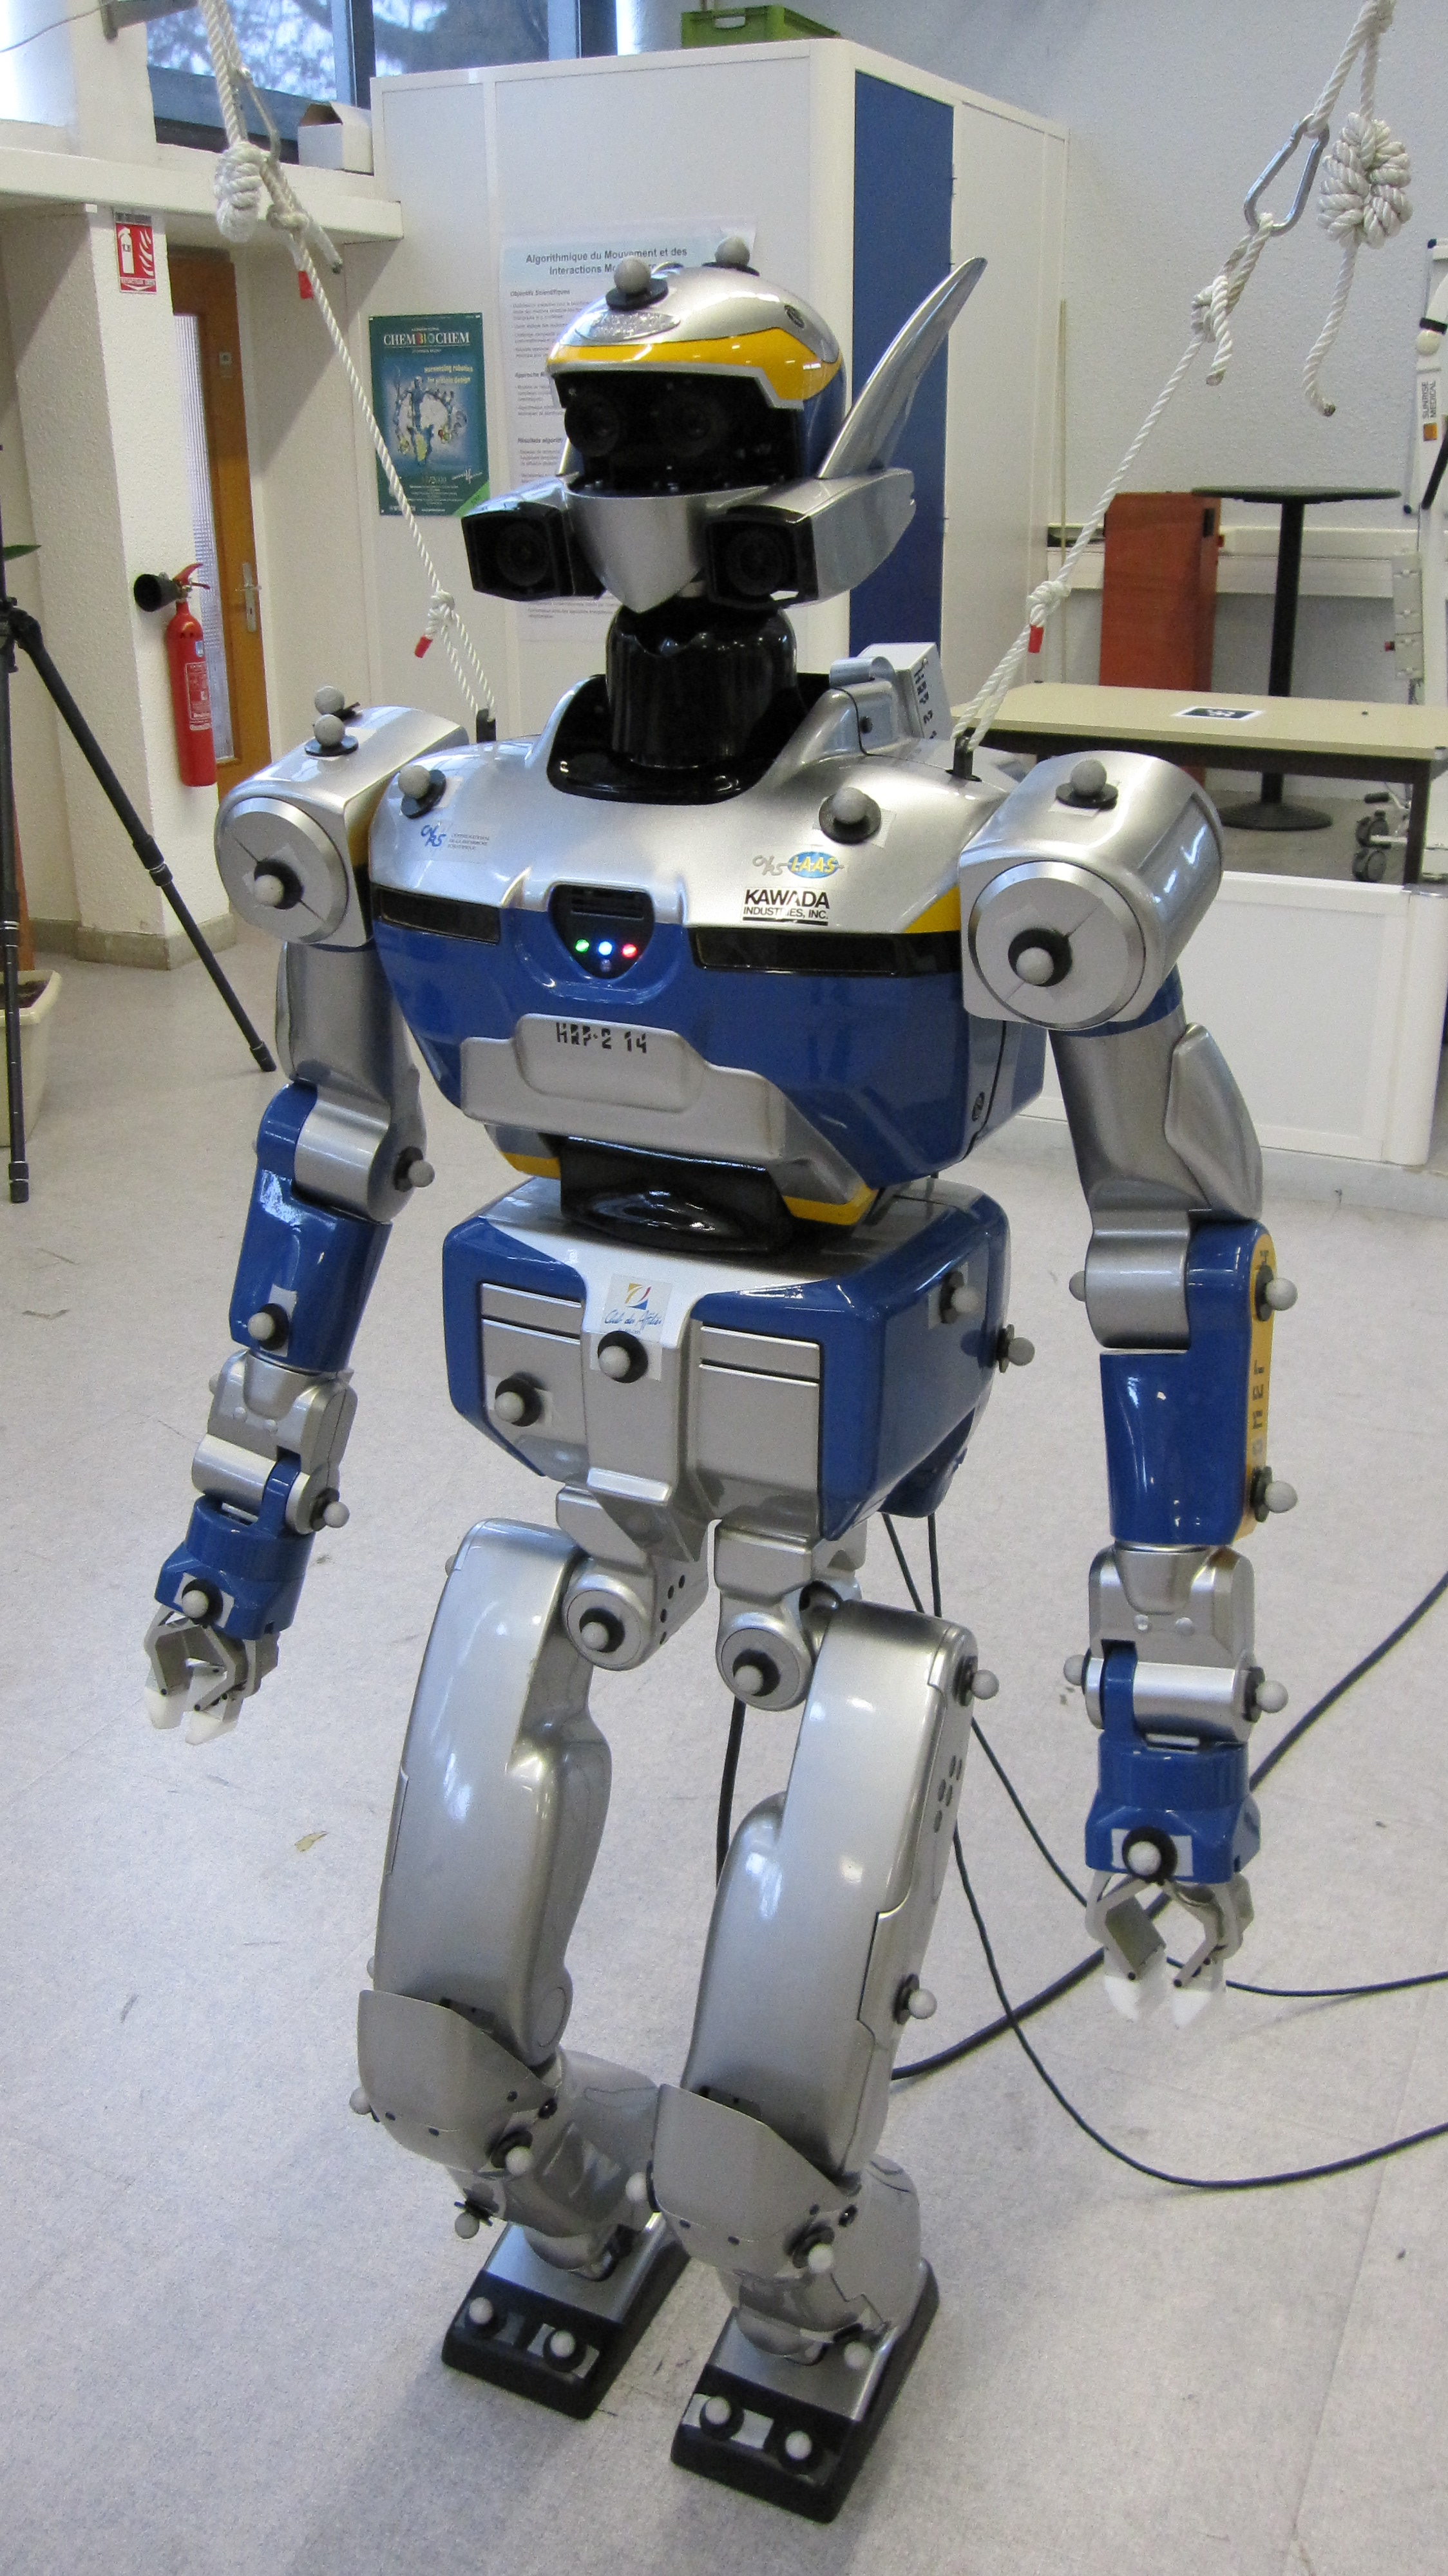
\includegraphics[height=0.7\linewidth]{img/hrp2Markers.ps} &
    \includegraphics[height=0.7\linewidth]{img/skel.ps} \\
  \end{tabular}
  \caption{Markers set and virtual skeleton of HRP2.}
  \label{fig:hrp2Markers}
\end{figure}

The computation of the trajectory of the motion in the joint angle space
of the robot is done by optimization.
In order to estimate the joint angle trajectory of the robot, a mapping between
the kinematic model of the robot and the kinematic model of the virtual skeleton
has to be made. Then the joint angle that would bring the robot to the same posture
as the skeleton is the joint angle that minimize the distance between
the transformation from the measured skeleton kinematic transformation to the robot kinematic model.
\begin{equation}
  \mbf{q}^*_i = \underset{\mbf{q}_i}\argmin \Vert K_W\tensor[^{0M}]{R}{_{iM}}K_i \ominus \tensor[^W]{R}{_{iQ}}(\mbf{q}_i) \Vert ^2\\
  \label{mocapOpti}
\end{equation}
where $K_W$ is the transformation matrix from the origin of the reference of the robot model to the reference of the 
motion capture data. $\tensor[^{0M}]{R}{_{iM}}$ is the transformation matrix from the root of the virtual bone to
the bone $i$ in the motion capture reference. $K_i$ is the transformation matrix from the virtual bone $i$ to
the corresponding joint of the robot model and $\tensor[^W]{R}{_{iQ}}$ is the transformation matrix from 
the origin of the reference of the robot model to the joint $i$ in the robot model reference.
$K_W$ and $K_i$ are constant and are computed in a calibration step where both real joint angle and
measured skeleton are known.

Joint angle trajectory are needed by the algorithm.

\begin{itemize}
  \item Both hands versus one hand
  \item Grab blind, Grab and look
  \item Grab, screw
\end{itemize}

\subsection{Right hand VS Both hands motion}
On the real robot, the flexibility of the ankles interfer with the motion at the very beginning as the acceleration
of the joint angle increase quickly. The flexibility is not modeled in our algorithm, so
in order to bypass the influence of the flexibility, the motion analysis is done after the first 100ms.

Tab.~\ref{tab:spotDiffReal1} shows the result of the identification algorithm run on
the motion data of the \emph{right hand} and \ emph{both hands} motion.
\begin{table}[t]
  \centering
  \begin{tabular}{|c|c|c|c|}
    \hline
    Reference & Detected & $\int \Vert \dot{q}(t) \Vert ^2 dt$ & $\int \Vert P\dot{q}(t) \Vert ^2 dt$ \\
    \hline
    \begin{tabular}{c}
      Com\\
      Right Hand\\
      Twofeet\\
    \end{tabular}

    &

    \begin{tabular}{c}
      Com\\
      Right Hand\\
      Twofeet\\
    \end{tabular}

    & 0.104835 & 0.0482885 \\
    \hline
    \begin{tabular}{c}
      Com\\
      Left Hand\\
      Right Hand\\
      Twofeet\\
    \end{tabular}

    &
    \begin{tabular}{c}
      Com\\
      Left Hand\\
      Right Hand\\
      Twofeet\\
    \end{tabular}

    & 0.142293  & 0.0541836 \\
    \hline
  \end{tabular}
  \caption{Results of the task selection algorithm from the analysis of the \emph{right-only} motion and the \emph{both hands} motion on the real robot.}
  \label{tab:spotDiffReal1}
  \vspace{-20pt}
\end{table}

Fig.~\ref{fig:exp1:taskCom0}-\ref{fig:exp1:taskTwofeet0} shows the
fitting at the first iteration of the algorithm. For the \emph{right
hand} motion, the projection in the task of the right hand have a good
fit (Fig.~\ref{fig:exp1:taskRhand0:R}) with the model of the
task, whereas the left hand projection have a poor fitting
(Fig.~\ref{fig:exp1:taskLhand0:R}).

%%%%%%%%%%%%%%%%%%%%%

\begin{figure*}[t]
  \centering
  \subfigure[Right hand motion - iteration 0]{
  \resizebox{.48\textwidth}{!} {
  % GNUPLOT: LaTeX picture with Postscript
\begingroup
  \makeatletter
  \providecommand\color[2][]{%
    \GenericError{(gnuplot) \space\space\space\@spaces}{%
      Package color not loaded in conjunction with
      terminal option `colourtext'%
    }{See the gnuplot documentation for explanation.%
    }{Either use 'blacktext' in gnuplot or load the package
      color.sty in LaTeX.}%
    \renewcommand\color[2][]{}%
  }%
  \providecommand\includegraphics[2][]{%
    \GenericError{(gnuplot) \space\space\space\@spaces}{%
      Package graphicx or graphics not loaded%
    }{See the gnuplot documentation for explanation.%
    }{The gnuplot epslatex terminal needs graphicx.sty or graphics.sty.}%
    \renewcommand\includegraphics[2][]{}%
  }%
  \providecommand\rotatebox[2]{#2}%
  \@ifundefined{ifGPcolor}{%
    \newif\ifGPcolor
    \GPcolortrue
  }{}%
  \@ifundefined{ifGPblacktext}{%
    \newif\ifGPblacktext
    \GPblacktexttrue
  }{}%
  % define a \g@addto@macro without @ in the name:
  \let\gplgaddtomacro\g@addto@macro
  % define empty templates for all commands taking text:
  \gdef\gplbacktext{}%
  \gdef\gplfronttext{}%
  \makeatother
  \ifGPblacktext
    % no textcolor at all
    \def\colorrgb#1{}%
    \def\colorgray#1{}%
  \else
    % gray or color?
    \ifGPcolor
      \def\colorrgb#1{\color[rgb]{#1}}%
      \def\colorgray#1{\color[gray]{#1}}%
      \expandafter\def\csname LTw\endcsname{\color{white}}%
      \expandafter\def\csname LTb\endcsname{\color{black}}%
      \expandafter\def\csname LTa\endcsname{\color{black}}%
      \expandafter\def\csname LT0\endcsname{\color[rgb]{1,0,0}}%
      \expandafter\def\csname LT1\endcsname{\color[rgb]{0,1,0}}%
      \expandafter\def\csname LT2\endcsname{\color[rgb]{0,0,1}}%
      \expandafter\def\csname LT3\endcsname{\color[rgb]{1,0,1}}%
      \expandafter\def\csname LT4\endcsname{\color[rgb]{0,1,1}}%
      \expandafter\def\csname LT5\endcsname{\color[rgb]{1,1,0}}%
      \expandafter\def\csname LT6\endcsname{\color[rgb]{0,0,0}}%
      \expandafter\def\csname LT7\endcsname{\color[rgb]{1,0.3,0}}%
      \expandafter\def\csname LT8\endcsname{\color[rgb]{0.5,0.5,0.5}}%
    \else
      % gray
      \def\colorrgb#1{\color{black}}%
      \def\colorgray#1{\color[gray]{#1}}%
      \expandafter\def\csname LTw\endcsname{\color{white}}%
      \expandafter\def\csname LTb\endcsname{\color{black}}%
      \expandafter\def\csname LTa\endcsname{\color{black}}%
      \expandafter\def\csname LT0\endcsname{\color{black}}%
      \expandafter\def\csname LT1\endcsname{\color{black}}%
      \expandafter\def\csname LT2\endcsname{\color{black}}%
      \expandafter\def\csname LT3\endcsname{\color{black}}%
      \expandafter\def\csname LT4\endcsname{\color{black}}%
      \expandafter\def\csname LT5\endcsname{\color{black}}%
      \expandafter\def\csname LT6\endcsname{\color{black}}%
      \expandafter\def\csname LT7\endcsname{\color{black}}%
      \expandafter\def\csname LT8\endcsname{\color{black}}%
    \fi
  \fi
  \setlength{\unitlength}{0.0500bp}%
  \begin{picture}(7200.00,5040.00)%
    \gplgaddtomacro\gplbacktext{%
      \csname LTb\endcsname%
      \put(1342,704){\makebox(0,0)[r]{\strut{} 0}}%
      \put(1342,1194){\makebox(0,0)[r]{\strut{} 0.01}}%
      \put(1342,1684){\makebox(0,0)[r]{\strut{} 0.02}}%
      \put(1342,2174){\makebox(0,0)[r]{\strut{} 0.03}}%
      \put(1342,2665){\makebox(0,0)[r]{\strut{} 0.04}}%
      \put(1342,3155){\makebox(0,0)[r]{\strut{} 0.05}}%
      \put(1342,3645){\makebox(0,0)[r]{\strut{} 0.06}}%
      \put(1342,4135){\makebox(0,0)[r]{\strut{} 0.07}}%
      \put(1474,484){\makebox(0,0){\strut{} 0}}%
      \put(2245,484){\makebox(0,0){\strut{} 2}}%
      \put(3016,484){\makebox(0,0){\strut{} 4}}%
      \put(3787,484){\makebox(0,0){\strut{} 6}}%
      \put(4557,484){\makebox(0,0){\strut{} 8}}%
      \put(5328,484){\makebox(0,0){\strut{} 10}}%
      \put(6099,484){\makebox(0,0){\strut{} 12}}%
      \put(6870,484){\makebox(0,0){\strut{} 14}}%
      \put(440,2542){\rotatebox{90}{\makebox(0,0){\strut{}$\Vert \dot{q}\Vert$ (rad/s)}}}%
      \put(4172,154){\makebox(0,0){\strut{}$t$ (s)}}%
      \put(4172,4710){\makebox(0,0){\strut{}Right hand motion - Com task}}%
    }%
    \gplgaddtomacro\gplfronttext{%
      \csname LTb\endcsname%
      \put(5883,4207){\makebox(0,0)[r]{\strut{}$J^+ \dot{e}_{com}$}}%
      \csname LTb\endcsname%
      \put(5883,3987){\makebox(0,0)[r]{\strut{}Model}}%
    }%
    \gplbacktext
    \put(0,0){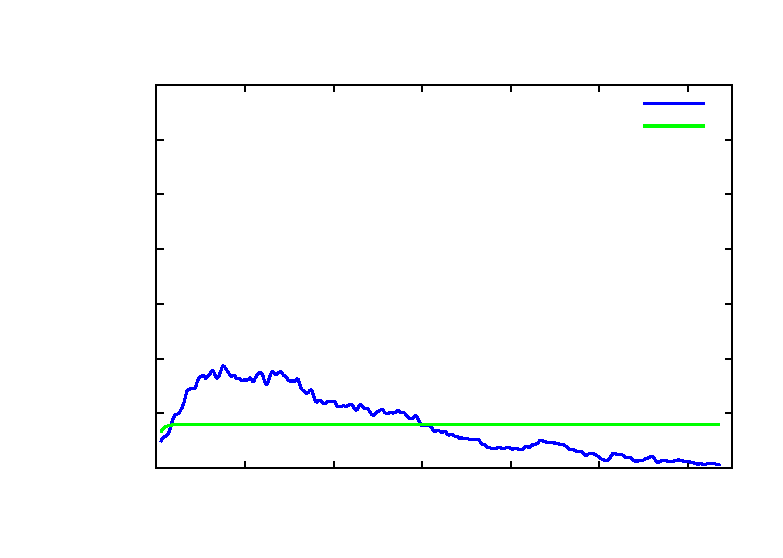
\includegraphics{img/exp1/R/invJerror_taskCom_0}}%
    \gplfronttext
  \end{picture}%
\endgroup

  }
  \label{fig:exp1:taskCom0:R}
  }
  \subfigure[Both hands motion - iteration 0]{
  \resizebox{.48\textwidth}{!} {
  % GNUPLOT: LaTeX picture with Postscript
\begingroup
  \makeatletter
  \providecommand\color[2][]{%
    \GenericError{(gnuplot) \space\space\space\@spaces}{%
      Package color not loaded in conjunction with
      terminal option `colourtext'%
    }{See the gnuplot documentation for explanation.%
    }{Either use 'blacktext' in gnuplot or load the package
      color.sty in LaTeX.}%
    \renewcommand\color[2][]{}%
  }%
  \providecommand\includegraphics[2][]{%
    \GenericError{(gnuplot) \space\space\space\@spaces}{%
      Package graphicx or graphics not loaded%
    }{See the gnuplot documentation for explanation.%
    }{The gnuplot epslatex terminal needs graphicx.sty or graphics.sty.}%
    \renewcommand\includegraphics[2][]{}%
  }%
  \providecommand\rotatebox[2]{#2}%
  \@ifundefined{ifGPcolor}{%
    \newif\ifGPcolor
    \GPcolortrue
  }{}%
  \@ifundefined{ifGPblacktext}{%
    \newif\ifGPblacktext
    \GPblacktexttrue
  }{}%
  % define a \g@addto@macro without @ in the name:
  \let\gplgaddtomacro\g@addto@macro
  % define empty templates for all commands taking text:
  \gdef\gplbacktext{}%
  \gdef\gplfronttext{}%
  \makeatother
  \ifGPblacktext
    % no textcolor at all
    \def\colorrgb#1{}%
    \def\colorgray#1{}%
  \else
    % gray or color?
    \ifGPcolor
      \def\colorrgb#1{\color[rgb]{#1}}%
      \def\colorgray#1{\color[gray]{#1}}%
      \expandafter\def\csname LTw\endcsname{\color{white}}%
      \expandafter\def\csname LTb\endcsname{\color{black}}%
      \expandafter\def\csname LTa\endcsname{\color{black}}%
      \expandafter\def\csname LT0\endcsname{\color[rgb]{1,0,0}}%
      \expandafter\def\csname LT1\endcsname{\color[rgb]{0,1,0}}%
      \expandafter\def\csname LT2\endcsname{\color[rgb]{0,0,1}}%
      \expandafter\def\csname LT3\endcsname{\color[rgb]{1,0,1}}%
      \expandafter\def\csname LT4\endcsname{\color[rgb]{0,1,1}}%
      \expandafter\def\csname LT5\endcsname{\color[rgb]{1,1,0}}%
      \expandafter\def\csname LT6\endcsname{\color[rgb]{0,0,0}}%
      \expandafter\def\csname LT7\endcsname{\color[rgb]{1,0.3,0}}%
      \expandafter\def\csname LT8\endcsname{\color[rgb]{0.5,0.5,0.5}}%
    \else
      % gray
      \def\colorrgb#1{\color{black}}%
      \def\colorgray#1{\color[gray]{#1}}%
      \expandafter\def\csname LTw\endcsname{\color{white}}%
      \expandafter\def\csname LTb\endcsname{\color{black}}%
      \expandafter\def\csname LTa\endcsname{\color{black}}%
      \expandafter\def\csname LT0\endcsname{\color{black}}%
      \expandafter\def\csname LT1\endcsname{\color{black}}%
      \expandafter\def\csname LT2\endcsname{\color{black}}%
      \expandafter\def\csname LT3\endcsname{\color{black}}%
      \expandafter\def\csname LT4\endcsname{\color{black}}%
      \expandafter\def\csname LT5\endcsname{\color{black}}%
      \expandafter\def\csname LT6\endcsname{\color{black}}%
      \expandafter\def\csname LT7\endcsname{\color{black}}%
      \expandafter\def\csname LT8\endcsname{\color{black}}%
    \fi
  \fi
  \setlength{\unitlength}{0.0500bp}%
  \begin{picture}(7200.00,5040.00)%
    \gplgaddtomacro\gplbacktext{%
      \csname LTb\endcsname%
      \put(1210,704){\makebox(0,0)[r]{\strut{} 0}}%
      \put(1210,1229){\makebox(0,0)[r]{\strut{} 0.1}}%
      \put(1210,1754){\makebox(0,0)[r]{\strut{} 0.2}}%
      \put(1210,2279){\makebox(0,0)[r]{\strut{} 0.3}}%
      \put(1210,2805){\makebox(0,0)[r]{\strut{} 0.4}}%
      \put(1210,3330){\makebox(0,0)[r]{\strut{} 0.5}}%
      \put(1210,3855){\makebox(0,0)[r]{\strut{} 0.6}}%
      \put(1210,4380){\makebox(0,0)[r]{\strut{} 0.7}}%
      \put(1342,484){\makebox(0,0){\strut{} 0}}%
      \put(2192,484){\makebox(0,0){\strut{} 2}}%
      \put(3043,484){\makebox(0,0){\strut{} 4}}%
      \put(3893,484){\makebox(0,0){\strut{} 6}}%
      \put(4744,484){\makebox(0,0){\strut{} 8}}%
      \put(5594,484){\makebox(0,0){\strut{} 10}}%
      \put(6445,484){\makebox(0,0){\strut{} 12}}%
      \put(440,2542){\rotatebox{90}{\makebox(0,0){\strut{}$\Vert \dot{q}\Vert$ (rad/s)}}}%
      \put(4106,154){\makebox(0,0){\strut{}$t$ (s)}}%
      \put(4106,4710){\makebox(0,0){\strut{}$\begin{array}{rl} r &= 1.35263\\ \int \Vert J^+ \dot{e}_{com} \Vert \mathrm{d}t &=  0.0714267 \mathrm{rad}\\ \end{array}$}}%
    }%
    \gplgaddtomacro\gplfronttext{%
      \csname LTb\endcsname%
      \put(5883,4207){\makebox(0,0)[r]{\strut{}$J^+ \dot{e}_{com} / \int \Vert J^+ \dot{e}_{com} \Vert \mathrm{d}t$}}%
      \csname LTb\endcsname%
      \put(5883,3987){\makebox(0,0)[r]{\strut{}Model}}%
    }%
    \gplbacktext
    \put(0,0){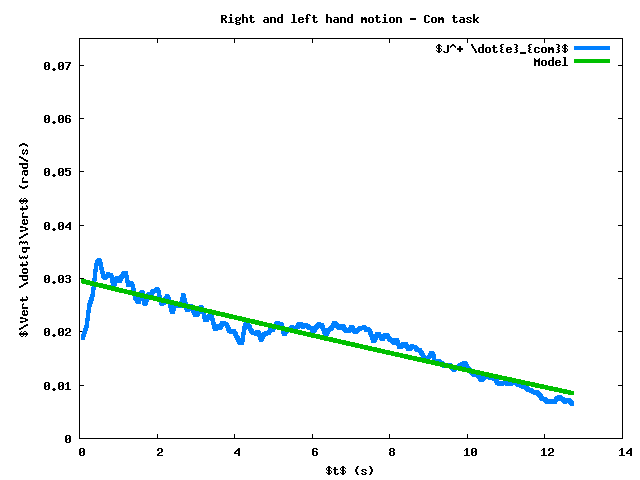
\includegraphics{img/exp1/RL/invJerror_taskCom_0}}%
    \gplfronttext
  \end{picture}%
\endgroup

  }
  \label{fig:exp1:taskCom0:RL}
  }
  \caption{Comparison of the fitting for the center of masses regulation task for the \emph{both hands} and \emph{right hand} motion at the first iteration of the identification algorithm.
  $r$ are the residues of the optimizations.}
  \label{fig:exp1:taskCom0}
\end{figure*}

satan satan satan satan satan satan satan satan satan satan satan
satan satan satan satan satan satan satan satan satan satan satan
satan satan satan satan satan satan satan satan satan satan satan
satan satan satan satan satan satan satan satan satan satan satan
satan satan satan satan satan satan satan satan satan satan satan

\begin{figure*}[t]
  \centering
  \subfigure[Right hand motion - iteration 0]{
  \resizebox{.48\textwidth}{!} {
  % GNUPLOT: LaTeX picture with Postscript
\begingroup
  \makeatletter
  \providecommand\color[2][]{%
    \GenericError{(gnuplot) \space\space\space\@spaces}{%
      Package color not loaded in conjunction with
      terminal option `colourtext'%
    }{See the gnuplot documentation for explanation.%
    }{Either use 'blacktext' in gnuplot or load the package
      color.sty in LaTeX.}%
    \renewcommand\color[2][]{}%
  }%
  \providecommand\includegraphics[2][]{%
    \GenericError{(gnuplot) \space\space\space\@spaces}{%
      Package graphicx or graphics not loaded%
    }{See the gnuplot documentation for explanation.%
    }{The gnuplot epslatex terminal needs graphicx.sty or graphics.sty.}%
    \renewcommand\includegraphics[2][]{}%
  }%
  \providecommand\rotatebox[2]{#2}%
  \@ifundefined{ifGPcolor}{%
    \newif\ifGPcolor
    \GPcolortrue
  }{}%
  \@ifundefined{ifGPblacktext}{%
    \newif\ifGPblacktext
    \GPblacktexttrue
  }{}%
  % define a \g@addto@macro without @ in the name:
  \let\gplgaddtomacro\g@addto@macro
  % define empty templates for all commands taking text:
  \gdef\gplbacktext{}%
  \gdef\gplfronttext{}%
  \makeatother
  \ifGPblacktext
    % no textcolor at all
    \def\colorrgb#1{}%
    \def\colorgray#1{}%
  \else
    % gray or color?
    \ifGPcolor
      \def\colorrgb#1{\color[rgb]{#1}}%
      \def\colorgray#1{\color[gray]{#1}}%
      \expandafter\def\csname LTw\endcsname{\color{white}}%
      \expandafter\def\csname LTb\endcsname{\color{black}}%
      \expandafter\def\csname LTa\endcsname{\color{black}}%
      \expandafter\def\csname LT0\endcsname{\color[rgb]{1,0,0}}%
      \expandafter\def\csname LT1\endcsname{\color[rgb]{0,1,0}}%
      \expandafter\def\csname LT2\endcsname{\color[rgb]{0,0,1}}%
      \expandafter\def\csname LT3\endcsname{\color[rgb]{1,0,1}}%
      \expandafter\def\csname LT4\endcsname{\color[rgb]{0,1,1}}%
      \expandafter\def\csname LT5\endcsname{\color[rgb]{1,1,0}}%
      \expandafter\def\csname LT6\endcsname{\color[rgb]{0,0,0}}%
      \expandafter\def\csname LT7\endcsname{\color[rgb]{1,0.3,0}}%
      \expandafter\def\csname LT8\endcsname{\color[rgb]{0.5,0.5,0.5}}%
    \else
      % gray
      \def\colorrgb#1{\color{black}}%
      \def\colorgray#1{\color[gray]{#1}}%
      \expandafter\def\csname LTw\endcsname{\color{white}}%
      \expandafter\def\csname LTb\endcsname{\color{black}}%
      \expandafter\def\csname LTa\endcsname{\color{black}}%
      \expandafter\def\csname LT0\endcsname{\color{black}}%
      \expandafter\def\csname LT1\endcsname{\color{black}}%
      \expandafter\def\csname LT2\endcsname{\color{black}}%
      \expandafter\def\csname LT3\endcsname{\color{black}}%
      \expandafter\def\csname LT4\endcsname{\color{black}}%
      \expandafter\def\csname LT5\endcsname{\color{black}}%
      \expandafter\def\csname LT6\endcsname{\color{black}}%
      \expandafter\def\csname LT7\endcsname{\color{black}}%
      \expandafter\def\csname LT8\endcsname{\color{black}}%
    \fi
  \fi
  \setlength{\unitlength}{0.0500bp}%
  \begin{picture}(7200.00,5040.00)%
    \gplgaddtomacro\gplbacktext{%
      \csname LTb\endcsname%
      \put(1210,704){\makebox(0,0)[r]{\strut{} 0}}%
      \put(1210,1229){\makebox(0,0)[r]{\strut{} 0.1}}%
      \put(1210,1754){\makebox(0,0)[r]{\strut{} 0.2}}%
      \put(1210,2279){\makebox(0,0)[r]{\strut{} 0.3}}%
      \put(1210,2805){\makebox(0,0)[r]{\strut{} 0.4}}%
      \put(1210,3330){\makebox(0,0)[r]{\strut{} 0.5}}%
      \put(1210,3855){\makebox(0,0)[r]{\strut{} 0.6}}%
      \put(1210,4380){\makebox(0,0)[r]{\strut{} 0.7}}%
      \put(1342,484){\makebox(0,0){\strut{} 0}}%
      \put(2192,484){\makebox(0,0){\strut{} 2}}%
      \put(3043,484){\makebox(0,0){\strut{} 4}}%
      \put(3893,484){\makebox(0,0){\strut{} 6}}%
      \put(4744,484){\makebox(0,0){\strut{} 8}}%
      \put(5594,484){\makebox(0,0){\strut{} 10}}%
      \put(6445,484){\makebox(0,0){\strut{} 12}}%
      \put(440,2542){\rotatebox{90}{\makebox(0,0){\strut{}$\Vert \dot{q}\Vert$ (rad/s)}}}%
      \put(4106,154){\makebox(0,0){\strut{}$t$ (s)}}%
      \put(4106,4710){\makebox(0,0){\strut{}$\begin{array}{rl} r &= 2.81959\\ \int \Vert J^+ \dot{e}_{head} \Vert \mathrm{d}t &=  0.0355852 \mathrm{rad}\\ \end{array}$}}%
    }%
    \gplgaddtomacro\gplfronttext{%
      \csname LTb\endcsname%
      \put(5883,4207){\makebox(0,0)[r]{\strut{}$J^+ \dot{e}_{head} / \int \Vert J^+ \dot{e}_{head} \Vert \mathrm{d}t$}}%
      \csname LTb\endcsname%
      \put(5883,3987){\makebox(0,0)[r]{\strut{}Model}}%
    }%
    \gplbacktext
    \put(0,0){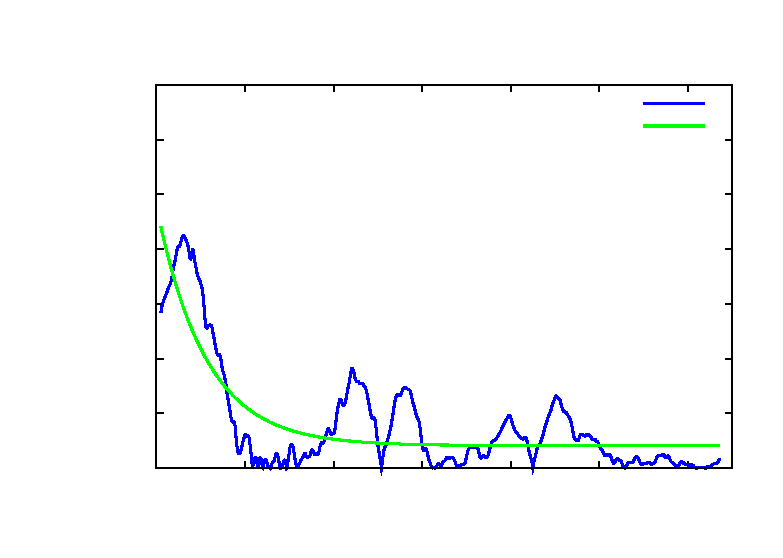
\includegraphics{img/exp1/R/invJerror_taskHead_0}}%
    \gplfronttext
  \end{picture}%
\endgroup

  }                           
  \label{fig:exp1:taskHead0:R}
  }
  \subfigure[Both hands motion - iteration 0]{
  \resizebox{.48\textwidth}{!} {
  % GNUPLOT: LaTeX picture with Postscript
\begingroup
  \makeatletter
  \providecommand\color[2][]{%
    \GenericError{(gnuplot) \space\space\space\@spaces}{%
      Package color not loaded in conjunction with
      terminal option `colourtext'%
    }{See the gnuplot documentation for explanation.%
    }{Either use 'blacktext' in gnuplot or load the package
      color.sty in LaTeX.}%
    \renewcommand\color[2][]{}%
  }%
  \providecommand\includegraphics[2][]{%
    \GenericError{(gnuplot) \space\space\space\@spaces}{%
      Package graphicx or graphics not loaded%
    }{See the gnuplot documentation for explanation.%
    }{The gnuplot epslatex terminal needs graphicx.sty or graphics.sty.}%
    \renewcommand\includegraphics[2][]{}%
  }%
  \providecommand\rotatebox[2]{#2}%
  \@ifundefined{ifGPcolor}{%
    \newif\ifGPcolor
    \GPcolortrue
  }{}%
  \@ifundefined{ifGPblacktext}{%
    \newif\ifGPblacktext
    \GPblacktexttrue
  }{}%
  % define a \g@addto@macro without @ in the name:
  \let\gplgaddtomacro\g@addto@macro
  % define empty templates for all commands taking text:
  \gdef\gplbacktext{}%
  \gdef\gplfronttext{}%
  \makeatother
  \ifGPblacktext
    % no textcolor at all
    \def\colorrgb#1{}%
    \def\colorgray#1{}%
  \else
    % gray or color?
    \ifGPcolor
      \def\colorrgb#1{\color[rgb]{#1}}%
      \def\colorgray#1{\color[gray]{#1}}%
      \expandafter\def\csname LTw\endcsname{\color{white}}%
      \expandafter\def\csname LTb\endcsname{\color{black}}%
      \expandafter\def\csname LTa\endcsname{\color{black}}%
      \expandafter\def\csname LT0\endcsname{\color[rgb]{1,0,0}}%
      \expandafter\def\csname LT1\endcsname{\color[rgb]{0,1,0}}%
      \expandafter\def\csname LT2\endcsname{\color[rgb]{0,0,1}}%
      \expandafter\def\csname LT3\endcsname{\color[rgb]{1,0,1}}%
      \expandafter\def\csname LT4\endcsname{\color[rgb]{0,1,1}}%
      \expandafter\def\csname LT5\endcsname{\color[rgb]{1,1,0}}%
      \expandafter\def\csname LT6\endcsname{\color[rgb]{0,0,0}}%
      \expandafter\def\csname LT7\endcsname{\color[rgb]{1,0.3,0}}%
      \expandafter\def\csname LT8\endcsname{\color[rgb]{0.5,0.5,0.5}}%
    \else
      % gray
      \def\colorrgb#1{\color{black}}%
      \def\colorgray#1{\color[gray]{#1}}%
      \expandafter\def\csname LTw\endcsname{\color{white}}%
      \expandafter\def\csname LTb\endcsname{\color{black}}%
      \expandafter\def\csname LTa\endcsname{\color{black}}%
      \expandafter\def\csname LT0\endcsname{\color{black}}%
      \expandafter\def\csname LT1\endcsname{\color{black}}%
      \expandafter\def\csname LT2\endcsname{\color{black}}%
      \expandafter\def\csname LT3\endcsname{\color{black}}%
      \expandafter\def\csname LT4\endcsname{\color{black}}%
      \expandafter\def\csname LT5\endcsname{\color{black}}%
      \expandafter\def\csname LT6\endcsname{\color{black}}%
      \expandafter\def\csname LT7\endcsname{\color{black}}%
      \expandafter\def\csname LT8\endcsname{\color{black}}%
    \fi
  \fi
  \setlength{\unitlength}{0.0500bp}%
  \begin{picture}(7200.00,5040.00)%
    \gplgaddtomacro\gplbacktext{%
      \csname LTb\endcsname%
      \put(1342,704){\makebox(0,0)[r]{\strut{} 0}}%
      \put(1342,1194){\makebox(0,0)[r]{\strut{} 0.01}}%
      \put(1342,1684){\makebox(0,0)[r]{\strut{} 0.02}}%
      \put(1342,2174){\makebox(0,0)[r]{\strut{} 0.03}}%
      \put(1342,2665){\makebox(0,0)[r]{\strut{} 0.04}}%
      \put(1342,3155){\makebox(0,0)[r]{\strut{} 0.05}}%
      \put(1342,3645){\makebox(0,0)[r]{\strut{} 0.06}}%
      \put(1342,4135){\makebox(0,0)[r]{\strut{} 0.07}}%
      \put(1474,484){\makebox(0,0){\strut{} 0}}%
      \put(2245,484){\makebox(0,0){\strut{} 2}}%
      \put(3016,484){\makebox(0,0){\strut{} 4}}%
      \put(3787,484){\makebox(0,0){\strut{} 6}}%
      \put(4557,484){\makebox(0,0){\strut{} 8}}%
      \put(5328,484){\makebox(0,0){\strut{} 10}}%
      \put(6099,484){\makebox(0,0){\strut{} 12}}%
      \put(6870,484){\makebox(0,0){\strut{} 14}}%
      \put(440,2542){\rotatebox{90}{\makebox(0,0){\strut{}$\Vert \dot{q}\Vert$ (rad/s)}}}%
      \put(4172,154){\makebox(0,0){\strut{}$t$ (s)}}%
      \put(4172,4710){\makebox(0,0){\strut{}Right and left hand motion - Head task}}%
    }%
    \gplgaddtomacro\gplfronttext{%
      \csname LTb\endcsname%
      \put(5883,4207){\makebox(0,0)[r]{\strut{}$J^+ \dot{e}_{head}$}}%
      \csname LTb\endcsname%
      \put(5883,3987){\makebox(0,0)[r]{\strut{}Model}}%
    }%
    \gplbacktext
    \put(0,0){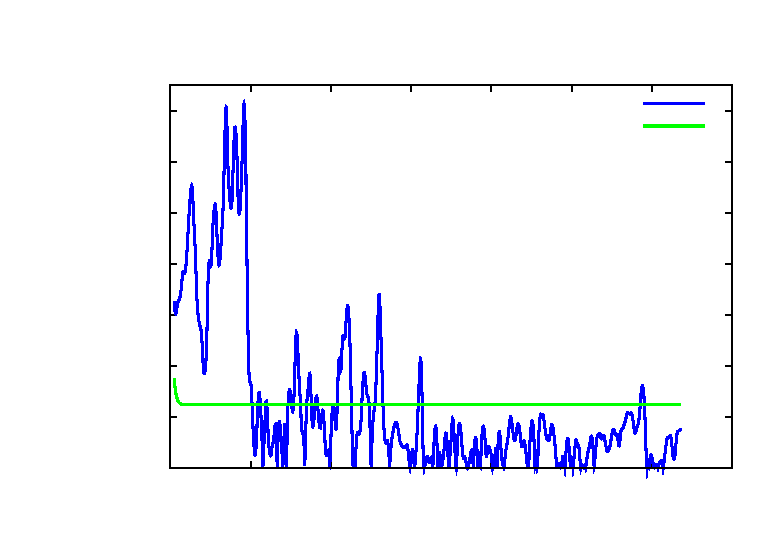
\includegraphics{img/exp1/RL/invJerror_taskHead_0}}%
    \gplfronttext
  \end{picture}%
\endgroup

  }
  \label{fig:exp1:taskHead0:RL}
  }
  \caption{Comparison of the fitting for the head task for the
  \emph{both hands} and \emph{right hand} motion at the first
  iteration of the identification algorithm.  $r$ are
  the residues of the optimizations.}
  \label{fig:exp1:taskHead0}
\end{figure*}

satan satan satan satan satan satan satan satan satan satan satan
satan satan satan satan satan satan satan satan satan satan satan
satan satan satan satan satan satan satan satan satan satan satan
satan satan satan satan satan satan satan satan satan satan satan

\begin{figure*}[t]
  \centering
  \subfigure[Right hand motion - iteration 0]{
  \resizebox{.48\textwidth}{!} {
  % GNUPLOT: LaTeX picture with Postscript
\begingroup
  \makeatletter
  \providecommand\color[2][]{%
    \GenericError{(gnuplot) \space\space\space\@spaces}{%
      Package color not loaded in conjunction with
      terminal option `colourtext'%
    }{See the gnuplot documentation for explanation.%
    }{Either use 'blacktext' in gnuplot or load the package
      color.sty in LaTeX.}%
    \renewcommand\color[2][]{}%
  }%
  \providecommand\includegraphics[2][]{%
    \GenericError{(gnuplot) \space\space\space\@spaces}{%
      Package graphicx or graphics not loaded%
    }{See the gnuplot documentation for explanation.%
    }{The gnuplot epslatex terminal needs graphicx.sty or graphics.sty.}%
    \renewcommand\includegraphics[2][]{}%
  }%
  \providecommand\rotatebox[2]{#2}%
  \@ifundefined{ifGPcolor}{%
    \newif\ifGPcolor
    \GPcolortrue
  }{}%
  \@ifundefined{ifGPblacktext}{%
    \newif\ifGPblacktext
    \GPblacktexttrue
  }{}%
  % define a \g@addto@macro without @ in the name:
  \let\gplgaddtomacro\g@addto@macro
  % define empty templates for all commands taking text:
  \gdef\gplbacktext{}%
  \gdef\gplfronttext{}%
  \makeatother
  \ifGPblacktext
    % no textcolor at all
    \def\colorrgb#1{}%
    \def\colorgray#1{}%
  \else
    % gray or color?
    \ifGPcolor
      \def\colorrgb#1{\color[rgb]{#1}}%
      \def\colorgray#1{\color[gray]{#1}}%
      \expandafter\def\csname LTw\endcsname{\color{white}}%
      \expandafter\def\csname LTb\endcsname{\color{black}}%
      \expandafter\def\csname LTa\endcsname{\color{black}}%
      \expandafter\def\csname LT0\endcsname{\color[rgb]{1,0,0}}%
      \expandafter\def\csname LT1\endcsname{\color[rgb]{0,1,0}}%
      \expandafter\def\csname LT2\endcsname{\color[rgb]{0,0,1}}%
      \expandafter\def\csname LT3\endcsname{\color[rgb]{1,0,1}}%
      \expandafter\def\csname LT4\endcsname{\color[rgb]{0,1,1}}%
      \expandafter\def\csname LT5\endcsname{\color[rgb]{1,1,0}}%
      \expandafter\def\csname LT6\endcsname{\color[rgb]{0,0,0}}%
      \expandafter\def\csname LT7\endcsname{\color[rgb]{1,0.3,0}}%
      \expandafter\def\csname LT8\endcsname{\color[rgb]{0.5,0.5,0.5}}%
    \else
      % gray
      \def\colorrgb#1{\color{black}}%
      \def\colorgray#1{\color[gray]{#1}}%
      \expandafter\def\csname LTw\endcsname{\color{white}}%
      \expandafter\def\csname LTb\endcsname{\color{black}}%
      \expandafter\def\csname LTa\endcsname{\color{black}}%
      \expandafter\def\csname LT0\endcsname{\color{black}}%
      \expandafter\def\csname LT1\endcsname{\color{black}}%
      \expandafter\def\csname LT2\endcsname{\color{black}}%
      \expandafter\def\csname LT3\endcsname{\color{black}}%
      \expandafter\def\csname LT4\endcsname{\color{black}}%
      \expandafter\def\csname LT5\endcsname{\color{black}}%
      \expandafter\def\csname LT6\endcsname{\color{black}}%
      \expandafter\def\csname LT7\endcsname{\color{black}}%
      \expandafter\def\csname LT8\endcsname{\color{black}}%
    \fi
  \fi
  \setlength{\unitlength}{0.0500bp}%
  \begin{picture}(7200.00,5040.00)%
    \gplgaddtomacro\gplbacktext{%
      \csname LTb\endcsname%
      \put(1342,704){\makebox(0,0)[r]{\strut{} 0}}%
      \put(1342,1194){\makebox(0,0)[r]{\strut{} 0.01}}%
      \put(1342,1684){\makebox(0,0)[r]{\strut{} 0.02}}%
      \put(1342,2174){\makebox(0,0)[r]{\strut{} 0.03}}%
      \put(1342,2665){\makebox(0,0)[r]{\strut{} 0.04}}%
      \put(1342,3155){\makebox(0,0)[r]{\strut{} 0.05}}%
      \put(1342,3645){\makebox(0,0)[r]{\strut{} 0.06}}%
      \put(1342,4135){\makebox(0,0)[r]{\strut{} 0.07}}%
      \put(1474,484){\makebox(0,0){\strut{} 0}}%
      \put(2245,484){\makebox(0,0){\strut{} 2}}%
      \put(3016,484){\makebox(0,0){\strut{} 4}}%
      \put(3787,484){\makebox(0,0){\strut{} 6}}%
      \put(4557,484){\makebox(0,0){\strut{} 8}}%
      \put(5328,484){\makebox(0,0){\strut{} 10}}%
      \put(6099,484){\makebox(0,0){\strut{} 12}}%
      \put(6870,484){\makebox(0,0){\strut{} 14}}%
      \put(440,2542){\rotatebox{90}{\makebox(0,0){\strut{}$\Vert \dot{q}\Vert$ (rad/s)}}}%
      \put(4172,154){\makebox(0,0){\strut{}$t$ (s)}}%
      \put(4172,4710){\makebox(0,0){\strut{}Right hand motion - Left Hand task}}%
    }%
    \gplgaddtomacro\gplfronttext{%
      \csname LTb\endcsname%
      \put(5883,4207){\makebox(0,0)[r]{\strut{}$J^+ \dot{e}_{lhand}$}}%
      \csname LTb\endcsname%
      \put(5883,3987){\makebox(0,0)[r]{\strut{}Model}}%
    }%
    \gplbacktext
    \put(0,0){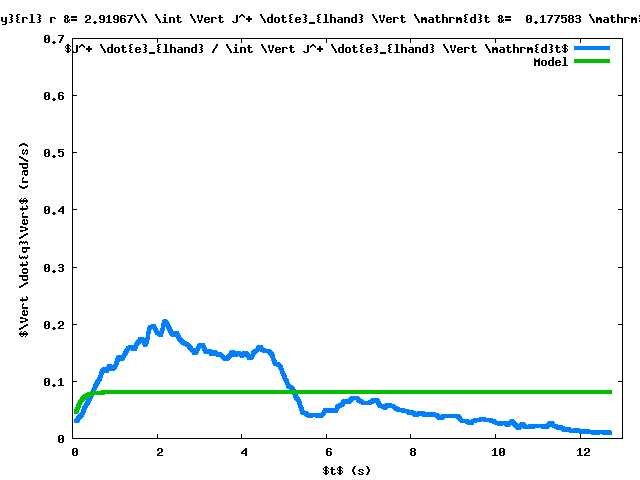
\includegraphics{img/exp1/R/invJerror_taskLhand_0}}%
    \gplfronttext
  \end{picture}%
\endgroup

  }
  \label{fig:exp1:taskLhand0:R}
  }
  \subfigure[Both hands motion - iteration 0]{
  \resizebox{.48\textwidth}{!} {
  % GNUPLOT: LaTeX picture with Postscript
\begingroup
  \makeatletter
  \providecommand\color[2][]{%
    \GenericError{(gnuplot) \space\space\space\@spaces}{%
      Package color not loaded in conjunction with
      terminal option `colourtext'%
    }{See the gnuplot documentation for explanation.%
    }{Either use 'blacktext' in gnuplot or load the package
      color.sty in LaTeX.}%
    \renewcommand\color[2][]{}%
  }%
  \providecommand\includegraphics[2][]{%
    \GenericError{(gnuplot) \space\space\space\@spaces}{%
      Package graphicx or graphics not loaded%
    }{See the gnuplot documentation for explanation.%
    }{The gnuplot epslatex terminal needs graphicx.sty or graphics.sty.}%
    \renewcommand\includegraphics[2][]{}%
  }%
  \providecommand\rotatebox[2]{#2}%
  \@ifundefined{ifGPcolor}{%
    \newif\ifGPcolor
    \GPcolortrue
  }{}%
  \@ifundefined{ifGPblacktext}{%
    \newif\ifGPblacktext
    \GPblacktexttrue
  }{}%
  % define a \g@addto@macro without @ in the name:
  \let\gplgaddtomacro\g@addto@macro
  % define empty templates for all commands taking text:
  \gdef\gplbacktext{}%
  \gdef\gplfronttext{}%
  \makeatother
  \ifGPblacktext
    % no textcolor at all
    \def\colorrgb#1{}%
    \def\colorgray#1{}%
  \else
    % gray or color?
    \ifGPcolor
      \def\colorrgb#1{\color[rgb]{#1}}%
      \def\colorgray#1{\color[gray]{#1}}%
      \expandafter\def\csname LTw\endcsname{\color{white}}%
      \expandafter\def\csname LTb\endcsname{\color{black}}%
      \expandafter\def\csname LTa\endcsname{\color{black}}%
      \expandafter\def\csname LT0\endcsname{\color[rgb]{1,0,0}}%
      \expandafter\def\csname LT1\endcsname{\color[rgb]{0,1,0}}%
      \expandafter\def\csname LT2\endcsname{\color[rgb]{0,0,1}}%
      \expandafter\def\csname LT3\endcsname{\color[rgb]{1,0,1}}%
      \expandafter\def\csname LT4\endcsname{\color[rgb]{0,1,1}}%
      \expandafter\def\csname LT5\endcsname{\color[rgb]{1,1,0}}%
      \expandafter\def\csname LT6\endcsname{\color[rgb]{0,0,0}}%
      \expandafter\def\csname LT7\endcsname{\color[rgb]{1,0.3,0}}%
      \expandafter\def\csname LT8\endcsname{\color[rgb]{0.5,0.5,0.5}}%
    \else
      % gray
      \def\colorrgb#1{\color{black}}%
      \def\colorgray#1{\color[gray]{#1}}%
      \expandafter\def\csname LTw\endcsname{\color{white}}%
      \expandafter\def\csname LTb\endcsname{\color{black}}%
      \expandafter\def\csname LTa\endcsname{\color{black}}%
      \expandafter\def\csname LT0\endcsname{\color{black}}%
      \expandafter\def\csname LT1\endcsname{\color{black}}%
      \expandafter\def\csname LT2\endcsname{\color{black}}%
      \expandafter\def\csname LT3\endcsname{\color{black}}%
      \expandafter\def\csname LT4\endcsname{\color{black}}%
      \expandafter\def\csname LT5\endcsname{\color{black}}%
      \expandafter\def\csname LT6\endcsname{\color{black}}%
      \expandafter\def\csname LT7\endcsname{\color{black}}%
      \expandafter\def\csname LT8\endcsname{\color{black}}%
    \fi
  \fi
  \setlength{\unitlength}{0.0500bp}%
  \begin{picture}(7200.00,5040.00)%
    \gplgaddtomacro\gplbacktext{%
      \csname LTb\endcsname%
      \put(1342,704){\makebox(0,0)[r]{\strut{} 0}}%
      \put(1342,1194){\makebox(0,0)[r]{\strut{} 0.01}}%
      \put(1342,1684){\makebox(0,0)[r]{\strut{} 0.02}}%
      \put(1342,2174){\makebox(0,0)[r]{\strut{} 0.03}}%
      \put(1342,2665){\makebox(0,0)[r]{\strut{} 0.04}}%
      \put(1342,3155){\makebox(0,0)[r]{\strut{} 0.05}}%
      \put(1342,3645){\makebox(0,0)[r]{\strut{} 0.06}}%
      \put(1342,4135){\makebox(0,0)[r]{\strut{} 0.07}}%
      \put(1474,484){\makebox(0,0){\strut{} 0}}%
      \put(2245,484){\makebox(0,0){\strut{} 2}}%
      \put(3016,484){\makebox(0,0){\strut{} 4}}%
      \put(3787,484){\makebox(0,0){\strut{} 6}}%
      \put(4557,484){\makebox(0,0){\strut{} 8}}%
      \put(5328,484){\makebox(0,0){\strut{} 10}}%
      \put(6099,484){\makebox(0,0){\strut{} 12}}%
      \put(6870,484){\makebox(0,0){\strut{} 14}}%
      \put(440,2542){\rotatebox{90}{\makebox(0,0){\strut{}$\Vert \dot{q}\Vert$ (rad/s)}}}%
      \put(4172,154){\makebox(0,0){\strut{}$t$ (s)}}%
      \put(4172,4710){\makebox(0,0){\strut{}Right and left hand motion - Left hand task}}%
    }%
    \gplgaddtomacro\gplfronttext{%
      \csname LTb\endcsname%
      \put(5883,4207){\makebox(0,0)[r]{\strut{}$J^+ \dot{e}_{lhand}$}}%
      \csname LTb\endcsname%
      \put(5883,3987){\makebox(0,0)[r]{\strut{}Model}}%
    }%
    \gplbacktext
    \put(0,0){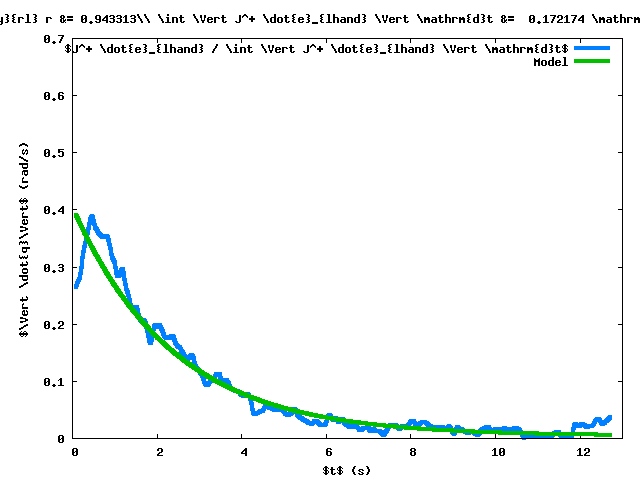
\includegraphics{img/exp1/RL/invJerror_taskLhand_0}}%
    \gplfronttext
  \end{picture}%
\endgroup

  }
  \label{fig:exp1:taskLhand0:RL}
  }
  \caption{Comparison of the fitting for the left hand task for the
  \emph{both hands} and \emph{right hand} motion at the first
  iteration of the identification algorithm.  $r$ are
  the residues of the optimizations.}
  \label{fig:exp1:taskLhand0}
\end{figure*}

satan satan satan satan satan satan satan satan satan satan satan
satan satan satan satan satan satan satan satan satan satan satan
satan satan satan satan satan satan satan satan satan satan satan
satan satan satan satan satan satan satan satan satan satan satan
satan satan satan satan satan satan satan satan satan satan satan

\begin{figure*}[t]
  \centering
  \subfigure[Right hand motion - iteration 0]{
  \resizebox{.48\textwidth}{!} {
  % GNUPLOT: LaTeX picture with Postscript
\begingroup
  \makeatletter
  \providecommand\color[2][]{%
    \GenericError{(gnuplot) \space\space\space\@spaces}{%
      Package color not loaded in conjunction with
      terminal option `colourtext'%
    }{See the gnuplot documentation for explanation.%
    }{Either use 'blacktext' in gnuplot or load the package
      color.sty in LaTeX.}%
    \renewcommand\color[2][]{}%
  }%
  \providecommand\includegraphics[2][]{%
    \GenericError{(gnuplot) \space\space\space\@spaces}{%
      Package graphicx or graphics not loaded%
    }{See the gnuplot documentation for explanation.%
    }{The gnuplot epslatex terminal needs graphicx.sty or graphics.sty.}%
    \renewcommand\includegraphics[2][]{}%
  }%
  \providecommand\rotatebox[2]{#2}%
  \@ifundefined{ifGPcolor}{%
    \newif\ifGPcolor
    \GPcolortrue
  }{}%
  \@ifundefined{ifGPblacktext}{%
    \newif\ifGPblacktext
    \GPblacktexttrue
  }{}%
  % define a \g@addto@macro without @ in the name:
  \let\gplgaddtomacro\g@addto@macro
  % define empty templates for all commands taking text:
  \gdef\gplbacktext{}%
  \gdef\gplfronttext{}%
  \makeatother
  \ifGPblacktext
    % no textcolor at all
    \def\colorrgb#1{}%
    \def\colorgray#1{}%
  \else
    % gray or color?
    \ifGPcolor
      \def\colorrgb#1{\color[rgb]{#1}}%
      \def\colorgray#1{\color[gray]{#1}}%
      \expandafter\def\csname LTw\endcsname{\color{white}}%
      \expandafter\def\csname LTb\endcsname{\color{black}}%
      \expandafter\def\csname LTa\endcsname{\color{black}}%
      \expandafter\def\csname LT0\endcsname{\color[rgb]{1,0,0}}%
      \expandafter\def\csname LT1\endcsname{\color[rgb]{0,1,0}}%
      \expandafter\def\csname LT2\endcsname{\color[rgb]{0,0,1}}%
      \expandafter\def\csname LT3\endcsname{\color[rgb]{1,0,1}}%
      \expandafter\def\csname LT4\endcsname{\color[rgb]{0,1,1}}%
      \expandafter\def\csname LT5\endcsname{\color[rgb]{1,1,0}}%
      \expandafter\def\csname LT6\endcsname{\color[rgb]{0,0,0}}%
      \expandafter\def\csname LT7\endcsname{\color[rgb]{1,0.3,0}}%
      \expandafter\def\csname LT8\endcsname{\color[rgb]{0.5,0.5,0.5}}%
    \else
      % gray
      \def\colorrgb#1{\color{black}}%
      \def\colorgray#1{\color[gray]{#1}}%
      \expandafter\def\csname LTw\endcsname{\color{white}}%
      \expandafter\def\csname LTb\endcsname{\color{black}}%
      \expandafter\def\csname LTa\endcsname{\color{black}}%
      \expandafter\def\csname LT0\endcsname{\color{black}}%
      \expandafter\def\csname LT1\endcsname{\color{black}}%
      \expandafter\def\csname LT2\endcsname{\color{black}}%
      \expandafter\def\csname LT3\endcsname{\color{black}}%
      \expandafter\def\csname LT4\endcsname{\color{black}}%
      \expandafter\def\csname LT5\endcsname{\color{black}}%
      \expandafter\def\csname LT6\endcsname{\color{black}}%
      \expandafter\def\csname LT7\endcsname{\color{black}}%
      \expandafter\def\csname LT8\endcsname{\color{black}}%
    \fi
  \fi
  \setlength{\unitlength}{0.0500bp}%
  \begin{picture}(7200.00,5040.00)%
    \gplgaddtomacro\gplbacktext{%
      \csname LTb\endcsname%
      \put(1342,704){\makebox(0,0)[r]{\strut{} 0}}%
      \put(1342,1194){\makebox(0,0)[r]{\strut{} 0.01}}%
      \put(1342,1684){\makebox(0,0)[r]{\strut{} 0.02}}%
      \put(1342,2174){\makebox(0,0)[r]{\strut{} 0.03}}%
      \put(1342,2665){\makebox(0,0)[r]{\strut{} 0.04}}%
      \put(1342,3155){\makebox(0,0)[r]{\strut{} 0.05}}%
      \put(1342,3645){\makebox(0,0)[r]{\strut{} 0.06}}%
      \put(1342,4135){\makebox(0,0)[r]{\strut{} 0.07}}%
      \put(1474,484){\makebox(0,0){\strut{} 0}}%
      \put(2245,484){\makebox(0,0){\strut{} 2}}%
      \put(3016,484){\makebox(0,0){\strut{} 4}}%
      \put(3787,484){\makebox(0,0){\strut{} 6}}%
      \put(4557,484){\makebox(0,0){\strut{} 8}}%
      \put(5328,484){\makebox(0,0){\strut{} 10}}%
      \put(6099,484){\makebox(0,0){\strut{} 12}}%
      \put(6870,484){\makebox(0,0){\strut{} 14}}%
      \put(440,2542){\rotatebox{90}{\makebox(0,0){\strut{}$\Vert \dot{q}\Vert$ (rad/s)}}}%
      \put(4172,154){\makebox(0,0){\strut{}$t$ (s)}}%
      \put(4172,4710){\makebox(0,0){\strut{}Right hand motion - Twofeet task}}%
    }%
    \gplgaddtomacro\gplfronttext{%
      \csname LTb\endcsname%
      \put(5883,4207){\makebox(0,0)[r]{\strut{}$J^+ \dot{e}_{twofeet}$}}%
      \csname LTb\endcsname%
      \put(5883,3987){\makebox(0,0)[r]{\strut{}Model}}%
    }%
    \gplbacktext
    \put(0,0){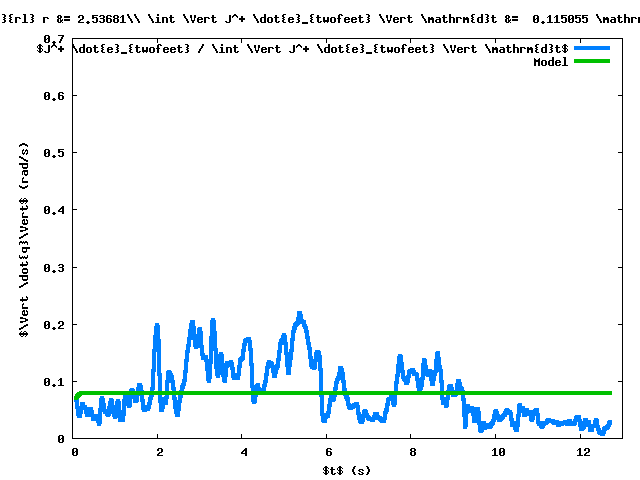
\includegraphics{img/exp1/R/invJerror_taskTwofeet_0}}%
    \gplfronttext
  \end{picture}%
\endgroup

  }
  \label{fig:exp1:taskTwofeet0:R}
  }
  \subfigure[Both hands motion - iteration 0]{
  \resizebox{.48\textwidth}{!} {
  % GNUPLOT: LaTeX picture with Postscript
\begingroup
  \makeatletter
  \providecommand\color[2][]{%
    \GenericError{(gnuplot) \space\space\space\@spaces}{%
      Package color not loaded in conjunction with
      terminal option `colourtext'%
    }{See the gnuplot documentation for explanation.%
    }{Either use 'blacktext' in gnuplot or load the package
      color.sty in LaTeX.}%
    \renewcommand\color[2][]{}%
  }%
  \providecommand\includegraphics[2][]{%
    \GenericError{(gnuplot) \space\space\space\@spaces}{%
      Package graphicx or graphics not loaded%
    }{See the gnuplot documentation for explanation.%
    }{The gnuplot epslatex terminal needs graphicx.sty or graphics.sty.}%
    \renewcommand\includegraphics[2][]{}%
  }%
  \providecommand\rotatebox[2]{#2}%
  \@ifundefined{ifGPcolor}{%
    \newif\ifGPcolor
    \GPcolortrue
  }{}%
  \@ifundefined{ifGPblacktext}{%
    \newif\ifGPblacktext
    \GPblacktexttrue
  }{}%
  % define a \g@addto@macro without @ in the name:
  \let\gplgaddtomacro\g@addto@macro
  % define empty templates for all commands taking text:
  \gdef\gplbacktext{}%
  \gdef\gplfronttext{}%
  \makeatother
  \ifGPblacktext
    % no textcolor at all
    \def\colorrgb#1{}%
    \def\colorgray#1{}%
  \else
    % gray or color?
    \ifGPcolor
      \def\colorrgb#1{\color[rgb]{#1}}%
      \def\colorgray#1{\color[gray]{#1}}%
      \expandafter\def\csname LTw\endcsname{\color{white}}%
      \expandafter\def\csname LTb\endcsname{\color{black}}%
      \expandafter\def\csname LTa\endcsname{\color{black}}%
      \expandafter\def\csname LT0\endcsname{\color[rgb]{1,0,0}}%
      \expandafter\def\csname LT1\endcsname{\color[rgb]{0,1,0}}%
      \expandafter\def\csname LT2\endcsname{\color[rgb]{0,0,1}}%
      \expandafter\def\csname LT3\endcsname{\color[rgb]{1,0,1}}%
      \expandafter\def\csname LT4\endcsname{\color[rgb]{0,1,1}}%
      \expandafter\def\csname LT5\endcsname{\color[rgb]{1,1,0}}%
      \expandafter\def\csname LT6\endcsname{\color[rgb]{0,0,0}}%
      \expandafter\def\csname LT7\endcsname{\color[rgb]{1,0.3,0}}%
      \expandafter\def\csname LT8\endcsname{\color[rgb]{0.5,0.5,0.5}}%
    \else
      % gray
      \def\colorrgb#1{\color{black}}%
      \def\colorgray#1{\color[gray]{#1}}%
      \expandafter\def\csname LTw\endcsname{\color{white}}%
      \expandafter\def\csname LTb\endcsname{\color{black}}%
      \expandafter\def\csname LTa\endcsname{\color{black}}%
      \expandafter\def\csname LT0\endcsname{\color{black}}%
      \expandafter\def\csname LT1\endcsname{\color{black}}%
      \expandafter\def\csname LT2\endcsname{\color{black}}%
      \expandafter\def\csname LT3\endcsname{\color{black}}%
      \expandafter\def\csname LT4\endcsname{\color{black}}%
      \expandafter\def\csname LT5\endcsname{\color{black}}%
      \expandafter\def\csname LT6\endcsname{\color{black}}%
      \expandafter\def\csname LT7\endcsname{\color{black}}%
      \expandafter\def\csname LT8\endcsname{\color{black}}%
    \fi
  \fi
  \setlength{\unitlength}{0.0500bp}%
  \begin{picture}(7200.00,5040.00)%
    \gplgaddtomacro\gplbacktext{%
      \csname LTb\endcsname%
      \put(1342,704){\makebox(0,0)[r]{\strut{} 0}}%
      \put(1342,1194){\makebox(0,0)[r]{\strut{} 0.01}}%
      \put(1342,1684){\makebox(0,0)[r]{\strut{} 0.02}}%
      \put(1342,2174){\makebox(0,0)[r]{\strut{} 0.03}}%
      \put(1342,2665){\makebox(0,0)[r]{\strut{} 0.04}}%
      \put(1342,3155){\makebox(0,0)[r]{\strut{} 0.05}}%
      \put(1342,3645){\makebox(0,0)[r]{\strut{} 0.06}}%
      \put(1342,4135){\makebox(0,0)[r]{\strut{} 0.07}}%
      \put(1474,484){\makebox(0,0){\strut{} 0}}%
      \put(2245,484){\makebox(0,0){\strut{} 2}}%
      \put(3016,484){\makebox(0,0){\strut{} 4}}%
      \put(3787,484){\makebox(0,0){\strut{} 6}}%
      \put(4557,484){\makebox(0,0){\strut{} 8}}%
      \put(5328,484){\makebox(0,0){\strut{} 10}}%
      \put(6099,484){\makebox(0,0){\strut{} 12}}%
      \put(6870,484){\makebox(0,0){\strut{} 14}}%
      \put(440,2542){\rotatebox{90}{\makebox(0,0){\strut{}$\Vert \dot{q}\Vert$ (rad/s)}}}%
      \put(4172,154){\makebox(0,0){\strut{}$t$ (s)}}%
      \put(4172,4710){\makebox(0,0){\strut{}Right and left hand motion - Twofeet task}}%
    }%
    \gplgaddtomacro\gplfronttext{%
      \csname LTb\endcsname%
      \put(5883,4207){\makebox(0,0)[r]{\strut{}$J^+ \dot{e}_{twofeet}$}}%
      \csname LTb\endcsname%
      \put(5883,3987){\makebox(0,0)[r]{\strut{}Model}}%
    }%
    \gplbacktext
    \put(0,0){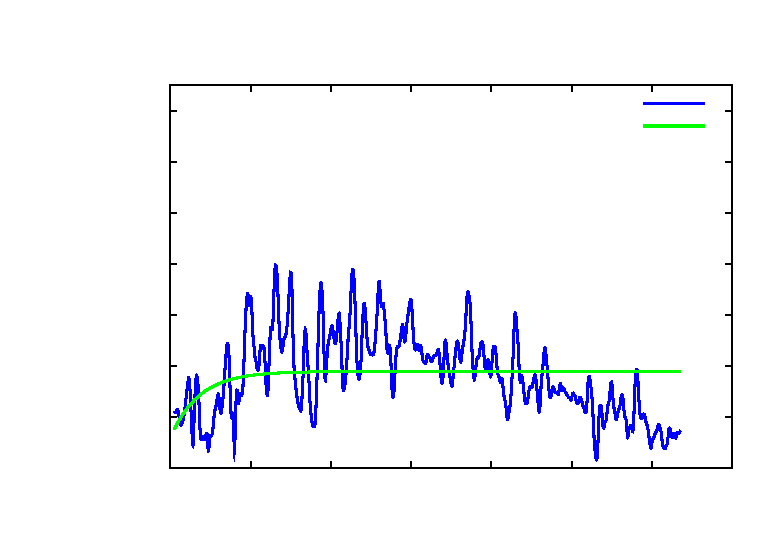
\includegraphics{img/exp1/RL/invJerror_taskTwofeet_0}}%
    \gplfronttext
  \end{picture}%
\endgroup

  }
  \label{fig:exp1:taskTwofeet0:RL}
  }
  \caption{Comparison of the fitting for the \emph{two feet} task for the
  \emph{both hands} and \emph{right hand} motion at the first
  iteration of the identification algorithm.  $r$ are the
  residues of the optimizations.}
  \label{fig:exp1:taskTwofeet0}
\end{figure*}

%%%%%%%%%%%%%%%%%%%%%%%%%%%%%%%%%%%%%%%%%%%%%%%5
satan satan satan satan satan satan satan satan satan satan satan
satan satan satan satan satan satan satan satan satan satan satan
satan satan satan satan satan satan satan satan satan satan satan
satan satan satan satan satan satan satan satan satan satan satan
satan satan satan satan satan satan satan satan satan satan satan

\begin{figure*}[t]
  \centering
  \subfigure[Right hand motion - iteration 1]{
  \resizebox{.48\textwidth}{!} {
	% GNUPLOT: LaTeX picture with Postscript
\begingroup
  \makeatletter
  \providecommand\color[2][]{%
    \GenericError{(gnuplot) \space\space\space\@spaces}{%
      Package color not loaded in conjunction with
      terminal option `colourtext'%
    }{See the gnuplot documentation for explanation.%
    }{Either use 'blacktext' in gnuplot or load the package
      color.sty in LaTeX.}%
    \renewcommand\color[2][]{}%
  }%
  \providecommand\includegraphics[2][]{%
    \GenericError{(gnuplot) \space\space\space\@spaces}{%
      Package graphicx or graphics not loaded%
    }{See the gnuplot documentation for explanation.%
    }{The gnuplot epslatex terminal needs graphicx.sty or graphics.sty.}%
    \renewcommand\includegraphics[2][]{}%
  }%
  \providecommand\rotatebox[2]{#2}%
  \@ifundefined{ifGPcolor}{%
    \newif\ifGPcolor
    \GPcolortrue
  }{}%
  \@ifundefined{ifGPblacktext}{%
    \newif\ifGPblacktext
    \GPblacktexttrue
  }{}%
  % define a \g@addto@macro without @ in the name:
  \let\gplgaddtomacro\g@addto@macro
  % define empty templates for all commands taking text:
  \gdef\gplbacktext{}%
  \gdef\gplfronttext{}%
  \makeatother
  \ifGPblacktext
    % no textcolor at all
    \def\colorrgb#1{}%
    \def\colorgray#1{}%
  \else
    % gray or color?
    \ifGPcolor
      \def\colorrgb#1{\color[rgb]{#1}}%
      \def\colorgray#1{\color[gray]{#1}}%
      \expandafter\def\csname LTw\endcsname{\color{white}}%
      \expandafter\def\csname LTb\endcsname{\color{black}}%
      \expandafter\def\csname LTa\endcsname{\color{black}}%
      \expandafter\def\csname LT0\endcsname{\color[rgb]{1,0,0}}%
      \expandafter\def\csname LT1\endcsname{\color[rgb]{0,1,0}}%
      \expandafter\def\csname LT2\endcsname{\color[rgb]{0,0,1}}%
      \expandafter\def\csname LT3\endcsname{\color[rgb]{1,0,1}}%
      \expandafter\def\csname LT4\endcsname{\color[rgb]{0,1,1}}%
      \expandafter\def\csname LT5\endcsname{\color[rgb]{1,1,0}}%
      \expandafter\def\csname LT6\endcsname{\color[rgb]{0,0,0}}%
      \expandafter\def\csname LT7\endcsname{\color[rgb]{1,0.3,0}}%
      \expandafter\def\csname LT8\endcsname{\color[rgb]{0.5,0.5,0.5}}%
    \else
      % gray
      \def\colorrgb#1{\color{black}}%
      \def\colorgray#1{\color[gray]{#1}}%
      \expandafter\def\csname LTw\endcsname{\color{white}}%
      \expandafter\def\csname LTb\endcsname{\color{black}}%
      \expandafter\def\csname LTa\endcsname{\color{black}}%
      \expandafter\def\csname LT0\endcsname{\color{black}}%
      \expandafter\def\csname LT1\endcsname{\color{black}}%
      \expandafter\def\csname LT2\endcsname{\color{black}}%
      \expandafter\def\csname LT3\endcsname{\color{black}}%
      \expandafter\def\csname LT4\endcsname{\color{black}}%
      \expandafter\def\csname LT5\endcsname{\color{black}}%
      \expandafter\def\csname LT6\endcsname{\color{black}}%
      \expandafter\def\csname LT7\endcsname{\color{black}}%
      \expandafter\def\csname LT8\endcsname{\color{black}}%
    \fi
  \fi
  \setlength{\unitlength}{0.0500bp}%
  \begin{picture}(7200.00,5040.00)%
    \gplgaddtomacro\gplbacktext{%
      \csname LTb\endcsname%
      \put(1342,704){\makebox(0,0)[r]{\strut{} 0}}%
      \put(1342,1194){\makebox(0,0)[r]{\strut{} 0.01}}%
      \put(1342,1684){\makebox(0,0)[r]{\strut{} 0.02}}%
      \put(1342,2174){\makebox(0,0)[r]{\strut{} 0.03}}%
      \put(1342,2665){\makebox(0,0)[r]{\strut{} 0.04}}%
      \put(1342,3155){\makebox(0,0)[r]{\strut{} 0.05}}%
      \put(1342,3645){\makebox(0,0)[r]{\strut{} 0.06}}%
      \put(1342,4135){\makebox(0,0)[r]{\strut{} 0.07}}%
      \put(1474,484){\makebox(0,0){\strut{} 0}}%
      \put(2245,484){\makebox(0,0){\strut{} 2}}%
      \put(3016,484){\makebox(0,0){\strut{} 4}}%
      \put(3787,484){\makebox(0,0){\strut{} 6}}%
      \put(4557,484){\makebox(0,0){\strut{} 8}}%
      \put(5328,484){\makebox(0,0){\strut{} 10}}%
      \put(6099,484){\makebox(0,0){\strut{} 12}}%
      \put(6870,484){\makebox(0,0){\strut{} 14}}%
      \put(440,2542){\rotatebox{90}{\makebox(0,0){\strut{}$\Vert \dot{q}\Vert$ (rad/s)}}}%
      \put(4172,154){\makebox(0,0){\strut{}$t$ (s)}}%
      \put(4172,4710){\makebox(0,0){\strut{}Right hand motion - Com task}}%
    }%
    \gplgaddtomacro\gplfronttext{%
      \csname LTb\endcsname%
      \put(5883,4207){\makebox(0,0)[r]{\strut{}$J^+ \dot{e}_{com}$}}%
      \csname LTb\endcsname%
      \put(5883,3987){\makebox(0,0)[r]{\strut{}Model}}%
    }%
    \gplbacktext
    \put(0,0){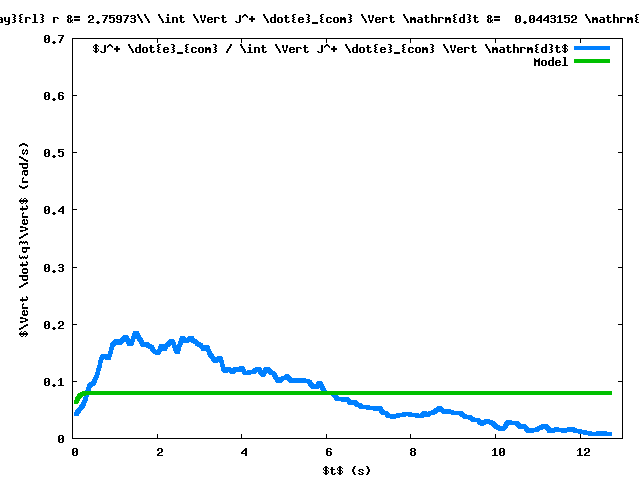
\includegraphics{img/exp1/R/invJerror_taskCom_1}}%
    \gplfronttext
  \end{picture}%
\endgroup

    }
    \label{fig:exp1:taskCom1:R}
  }
  \subfigure[Both hands motion - iteration 1]{
  \resizebox{.48\textwidth}{!} {
	% GNUPLOT: LaTeX picture with Postscript
\begingroup
  \makeatletter
  \providecommand\color[2][]{%
    \GenericError{(gnuplot) \space\space\space\@spaces}{%
      Package color not loaded in conjunction with
      terminal option `colourtext'%
    }{See the gnuplot documentation for explanation.%
    }{Either use 'blacktext' in gnuplot or load the package
      color.sty in LaTeX.}%
    \renewcommand\color[2][]{}%
  }%
  \providecommand\includegraphics[2][]{%
    \GenericError{(gnuplot) \space\space\space\@spaces}{%
      Package graphicx or graphics not loaded%
    }{See the gnuplot documentation for explanation.%
    }{The gnuplot epslatex terminal needs graphicx.sty or graphics.sty.}%
    \renewcommand\includegraphics[2][]{}%
  }%
  \providecommand\rotatebox[2]{#2}%
  \@ifundefined{ifGPcolor}{%
    \newif\ifGPcolor
    \GPcolortrue
  }{}%
  \@ifundefined{ifGPblacktext}{%
    \newif\ifGPblacktext
    \GPblacktexttrue
  }{}%
  % define a \g@addto@macro without @ in the name:
  \let\gplgaddtomacro\g@addto@macro
  % define empty templates for all commands taking text:
  \gdef\gplbacktext{}%
  \gdef\gplfronttext{}%
  \makeatother
  \ifGPblacktext
    % no textcolor at all
    \def\colorrgb#1{}%
    \def\colorgray#1{}%
  \else
    % gray or color?
    \ifGPcolor
      \def\colorrgb#1{\color[rgb]{#1}}%
      \def\colorgray#1{\color[gray]{#1}}%
      \expandafter\def\csname LTw\endcsname{\color{white}}%
      \expandafter\def\csname LTb\endcsname{\color{black}}%
      \expandafter\def\csname LTa\endcsname{\color{black}}%
      \expandafter\def\csname LT0\endcsname{\color[rgb]{1,0,0}}%
      \expandafter\def\csname LT1\endcsname{\color[rgb]{0,1,0}}%
      \expandafter\def\csname LT2\endcsname{\color[rgb]{0,0,1}}%
      \expandafter\def\csname LT3\endcsname{\color[rgb]{1,0,1}}%
      \expandafter\def\csname LT4\endcsname{\color[rgb]{0,1,1}}%
      \expandafter\def\csname LT5\endcsname{\color[rgb]{1,1,0}}%
      \expandafter\def\csname LT6\endcsname{\color[rgb]{0,0,0}}%
      \expandafter\def\csname LT7\endcsname{\color[rgb]{1,0.3,0}}%
      \expandafter\def\csname LT8\endcsname{\color[rgb]{0.5,0.5,0.5}}%
    \else
      % gray
      \def\colorrgb#1{\color{black}}%
      \def\colorgray#1{\color[gray]{#1}}%
      \expandafter\def\csname LTw\endcsname{\color{white}}%
      \expandafter\def\csname LTb\endcsname{\color{black}}%
      \expandafter\def\csname LTa\endcsname{\color{black}}%
      \expandafter\def\csname LT0\endcsname{\color{black}}%
      \expandafter\def\csname LT1\endcsname{\color{black}}%
      \expandafter\def\csname LT2\endcsname{\color{black}}%
      \expandafter\def\csname LT3\endcsname{\color{black}}%
      \expandafter\def\csname LT4\endcsname{\color{black}}%
      \expandafter\def\csname LT5\endcsname{\color{black}}%
      \expandafter\def\csname LT6\endcsname{\color{black}}%
      \expandafter\def\csname LT7\endcsname{\color{black}}%
      \expandafter\def\csname LT8\endcsname{\color{black}}%
    \fi
  \fi
  \setlength{\unitlength}{0.0500bp}%
  \begin{picture}(7200.00,5040.00)%
    \gplgaddtomacro\gplbacktext{%
      \csname LTb\endcsname%
      \put(1342,704){\makebox(0,0)[r]{\strut{} 0}}%
      \put(1342,1194){\makebox(0,0)[r]{\strut{} 0.01}}%
      \put(1342,1684){\makebox(0,0)[r]{\strut{} 0.02}}%
      \put(1342,2174){\makebox(0,0)[r]{\strut{} 0.03}}%
      \put(1342,2665){\makebox(0,0)[r]{\strut{} 0.04}}%
      \put(1342,3155){\makebox(0,0)[r]{\strut{} 0.05}}%
      \put(1342,3645){\makebox(0,0)[r]{\strut{} 0.06}}%
      \put(1342,4135){\makebox(0,0)[r]{\strut{} 0.07}}%
      \put(1474,484){\makebox(0,0){\strut{} 0}}%
      \put(2245,484){\makebox(0,0){\strut{} 2}}%
      \put(3016,484){\makebox(0,0){\strut{} 4}}%
      \put(3787,484){\makebox(0,0){\strut{} 6}}%
      \put(4557,484){\makebox(0,0){\strut{} 8}}%
      \put(5328,484){\makebox(0,0){\strut{} 10}}%
      \put(6099,484){\makebox(0,0){\strut{} 12}}%
      \put(6870,484){\makebox(0,0){\strut{} 14}}%
      \put(440,2542){\rotatebox{90}{\makebox(0,0){\strut{}$\Vert \dot{q}\Vert$ (rad/s)}}}%
      \put(4172,154){\makebox(0,0){\strut{}$t$ (s)}}%
      \put(4172,4710){\makebox(0,0){\strut{}Right and left hand motion - Com task}}%
    }%
    \gplgaddtomacro\gplfronttext{%
      \csname LTb\endcsname%
      \put(5883,4207){\makebox(0,0)[r]{\strut{}$J^+ \dot{e}_{com}$}}%
      \csname LTb\endcsname%
      \put(5883,3987){\makebox(0,0)[r]{\strut{}Model}}%
    }%
    \gplbacktext
    \put(0,0){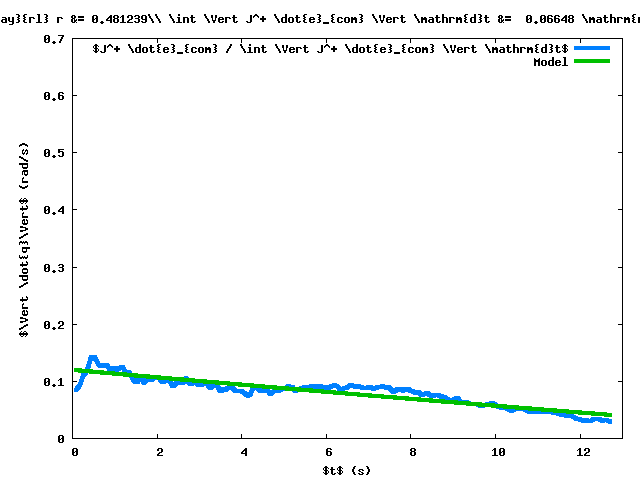
\includegraphics{img/exp1/RL/invJerror_taskCom_1}}%
    \gplfronttext
  \end{picture}%
\endgroup

    }
    \label{fig:exp1:taskCom1:RL}
  }
\caption{Comparison of the fitting for the center of masses regulation task for the \emph{both hands} and \emph{right hand} motion at the second iteration of the identification algorithm.
$r$ are the residues of the optimizations.}
\label{fig:exp1:taskCom1}
\end{figure*}

satan satan satan satan satan satan satan satan satan satan satan
satan satan satan satan satan satan satan satan satan satan satan
satan satan satan satan satan satan satan satan satan satan satan
satan satan satan satan satan satan satan satan satan satan satan
satan satan satan satan satan satan satan satan satan satan satan

\begin{figure*}[t]
  \centering
  \subfigure[Right hand motion - iteration 1]{
  \resizebox{.48\textwidth}{!} {
	% GNUPLOT: LaTeX picture with Postscript
\begingroup
  \makeatletter
  \providecommand\color[2][]{%
    \GenericError{(gnuplot) \space\space\space\@spaces}{%
      Package color not loaded in conjunction with
      terminal option `colourtext'%
    }{See the gnuplot documentation for explanation.%
    }{Either use 'blacktext' in gnuplot or load the package
      color.sty in LaTeX.}%
    \renewcommand\color[2][]{}%
  }%
  \providecommand\includegraphics[2][]{%
    \GenericError{(gnuplot) \space\space\space\@spaces}{%
      Package graphicx or graphics not loaded%
    }{See the gnuplot documentation for explanation.%
    }{The gnuplot epslatex terminal needs graphicx.sty or graphics.sty.}%
    \renewcommand\includegraphics[2][]{}%
  }%
  \providecommand\rotatebox[2]{#2}%
  \@ifundefined{ifGPcolor}{%
    \newif\ifGPcolor
    \GPcolortrue
  }{}%
  \@ifundefined{ifGPblacktext}{%
    \newif\ifGPblacktext
    \GPblacktexttrue
  }{}%
  % define a \g@addto@macro without @ in the name:
  \let\gplgaddtomacro\g@addto@macro
  % define empty templates for all commands taking text:
  \gdef\gplbacktext{}%
  \gdef\gplfronttext{}%
  \makeatother
  \ifGPblacktext
    % no textcolor at all
    \def\colorrgb#1{}%
    \def\colorgray#1{}%
  \else
    % gray or color?
    \ifGPcolor
      \def\colorrgb#1{\color[rgb]{#1}}%
      \def\colorgray#1{\color[gray]{#1}}%
      \expandafter\def\csname LTw\endcsname{\color{white}}%
      \expandafter\def\csname LTb\endcsname{\color{black}}%
      \expandafter\def\csname LTa\endcsname{\color{black}}%
      \expandafter\def\csname LT0\endcsname{\color[rgb]{1,0,0}}%
      \expandafter\def\csname LT1\endcsname{\color[rgb]{0,1,0}}%
      \expandafter\def\csname LT2\endcsname{\color[rgb]{0,0,1}}%
      \expandafter\def\csname LT3\endcsname{\color[rgb]{1,0,1}}%
      \expandafter\def\csname LT4\endcsname{\color[rgb]{0,1,1}}%
      \expandafter\def\csname LT5\endcsname{\color[rgb]{1,1,0}}%
      \expandafter\def\csname LT6\endcsname{\color[rgb]{0,0,0}}%
      \expandafter\def\csname LT7\endcsname{\color[rgb]{1,0.3,0}}%
      \expandafter\def\csname LT8\endcsname{\color[rgb]{0.5,0.5,0.5}}%
    \else
      % gray
      \def\colorrgb#1{\color{black}}%
      \def\colorgray#1{\color[gray]{#1}}%
      \expandafter\def\csname LTw\endcsname{\color{white}}%
      \expandafter\def\csname LTb\endcsname{\color{black}}%
      \expandafter\def\csname LTa\endcsname{\color{black}}%
      \expandafter\def\csname LT0\endcsname{\color{black}}%
      \expandafter\def\csname LT1\endcsname{\color{black}}%
      \expandafter\def\csname LT2\endcsname{\color{black}}%
      \expandafter\def\csname LT3\endcsname{\color{black}}%
      \expandafter\def\csname LT4\endcsname{\color{black}}%
      \expandafter\def\csname LT5\endcsname{\color{black}}%
      \expandafter\def\csname LT6\endcsname{\color{black}}%
      \expandafter\def\csname LT7\endcsname{\color{black}}%
      \expandafter\def\csname LT8\endcsname{\color{black}}%
    \fi
  \fi
  \setlength{\unitlength}{0.0500bp}%
  \begin{picture}(7200.00,5040.00)%
    \gplgaddtomacro\gplbacktext{%
      \csname LTb\endcsname%
      \put(1342,704){\makebox(0,0)[r]{\strut{} 0}}%
      \put(1342,1194){\makebox(0,0)[r]{\strut{} 0.01}}%
      \put(1342,1684){\makebox(0,0)[r]{\strut{} 0.02}}%
      \put(1342,2174){\makebox(0,0)[r]{\strut{} 0.03}}%
      \put(1342,2665){\makebox(0,0)[r]{\strut{} 0.04}}%
      \put(1342,3155){\makebox(0,0)[r]{\strut{} 0.05}}%
      \put(1342,3645){\makebox(0,0)[r]{\strut{} 0.06}}%
      \put(1342,4135){\makebox(0,0)[r]{\strut{} 0.07}}%
      \put(1474,484){\makebox(0,0){\strut{} 0}}%
      \put(2245,484){\makebox(0,0){\strut{} 2}}%
      \put(3016,484){\makebox(0,0){\strut{} 4}}%
      \put(3787,484){\makebox(0,0){\strut{} 6}}%
      \put(4557,484){\makebox(0,0){\strut{} 8}}%
      \put(5328,484){\makebox(0,0){\strut{} 10}}%
      \put(6099,484){\makebox(0,0){\strut{} 12}}%
      \put(6870,484){\makebox(0,0){\strut{} 14}}%
      \put(440,2542){\rotatebox{90}{\makebox(0,0){\strut{}$\Vert \dot{q}\Vert$ (rad/s)}}}%
      \put(4172,154){\makebox(0,0){\strut{}$t$ (s)}}%
      \put(4172,4710){\makebox(0,0){\strut{}Right hand motion - Head task}}%
    }%
    \gplgaddtomacro\gplfronttext{%
      \csname LTb\endcsname%
      \put(5883,4207){\makebox(0,0)[r]{\strut{}$J^+ \dot{e}_{head}$}}%
      \csname LTb\endcsname%
      \put(5883,3987){\makebox(0,0)[r]{\strut{}Model}}%
    }%
    \gplbacktext
    \put(0,0){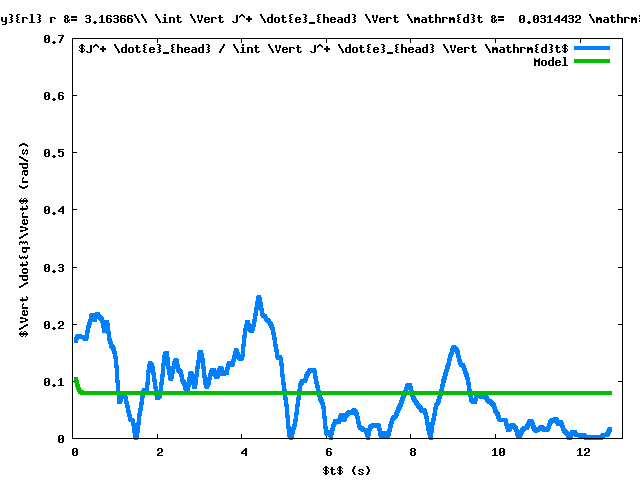
\includegraphics{img/exp1/R/invJerror_taskHead_1}}%
    \gplfronttext
  \end{picture}%
\endgroup

    } 
    \label{fig:exp1:taskHead1:R}
  }
  \subfigure[Both hands motion - iteration 1]{
  \resizebox{.48\textwidth}{!} {
	% GNUPLOT: LaTeX picture with Postscript
\begingroup
  \makeatletter
  \providecommand\color[2][]{%
    \GenericError{(gnuplot) \space\space\space\@spaces}{%
      Package color not loaded in conjunction with
      terminal option `colourtext'%
    }{See the gnuplot documentation for explanation.%
    }{Either use 'blacktext' in gnuplot or load the package
      color.sty in LaTeX.}%
    \renewcommand\color[2][]{}%
  }%
  \providecommand\includegraphics[2][]{%
    \GenericError{(gnuplot) \space\space\space\@spaces}{%
      Package graphicx or graphics not loaded%
    }{See the gnuplot documentation for explanation.%
    }{The gnuplot epslatex terminal needs graphicx.sty or graphics.sty.}%
    \renewcommand\includegraphics[2][]{}%
  }%
  \providecommand\rotatebox[2]{#2}%
  \@ifundefined{ifGPcolor}{%
    \newif\ifGPcolor
    \GPcolortrue
  }{}%
  \@ifundefined{ifGPblacktext}{%
    \newif\ifGPblacktext
    \GPblacktexttrue
  }{}%
  % define a \g@addto@macro without @ in the name:
  \let\gplgaddtomacro\g@addto@macro
  % define empty templates for all commands taking text:
  \gdef\gplbacktext{}%
  \gdef\gplfronttext{}%
  \makeatother
  \ifGPblacktext
    % no textcolor at all
    \def\colorrgb#1{}%
    \def\colorgray#1{}%
  \else
    % gray or color?
    \ifGPcolor
      \def\colorrgb#1{\color[rgb]{#1}}%
      \def\colorgray#1{\color[gray]{#1}}%
      \expandafter\def\csname LTw\endcsname{\color{white}}%
      \expandafter\def\csname LTb\endcsname{\color{black}}%
      \expandafter\def\csname LTa\endcsname{\color{black}}%
      \expandafter\def\csname LT0\endcsname{\color[rgb]{1,0,0}}%
      \expandafter\def\csname LT1\endcsname{\color[rgb]{0,1,0}}%
      \expandafter\def\csname LT2\endcsname{\color[rgb]{0,0,1}}%
      \expandafter\def\csname LT3\endcsname{\color[rgb]{1,0,1}}%
      \expandafter\def\csname LT4\endcsname{\color[rgb]{0,1,1}}%
      \expandafter\def\csname LT5\endcsname{\color[rgb]{1,1,0}}%
      \expandafter\def\csname LT6\endcsname{\color[rgb]{0,0,0}}%
      \expandafter\def\csname LT7\endcsname{\color[rgb]{1,0.3,0}}%
      \expandafter\def\csname LT8\endcsname{\color[rgb]{0.5,0.5,0.5}}%
    \else
      % gray
      \def\colorrgb#1{\color{black}}%
      \def\colorgray#1{\color[gray]{#1}}%
      \expandafter\def\csname LTw\endcsname{\color{white}}%
      \expandafter\def\csname LTb\endcsname{\color{black}}%
      \expandafter\def\csname LTa\endcsname{\color{black}}%
      \expandafter\def\csname LT0\endcsname{\color{black}}%
      \expandafter\def\csname LT1\endcsname{\color{black}}%
      \expandafter\def\csname LT2\endcsname{\color{black}}%
      \expandafter\def\csname LT3\endcsname{\color{black}}%
      \expandafter\def\csname LT4\endcsname{\color{black}}%
      \expandafter\def\csname LT5\endcsname{\color{black}}%
      \expandafter\def\csname LT6\endcsname{\color{black}}%
      \expandafter\def\csname LT7\endcsname{\color{black}}%
      \expandafter\def\csname LT8\endcsname{\color{black}}%
    \fi
  \fi
  \setlength{\unitlength}{0.0500bp}%
  \begin{picture}(7200.00,5040.00)%
    \gplgaddtomacro\gplbacktext{%
      \csname LTb\endcsname%
      \put(1210,704){\makebox(0,0)[r]{\strut{} 0}}%
      \put(1210,1229){\makebox(0,0)[r]{\strut{} 0.1}}%
      \put(1210,1754){\makebox(0,0)[r]{\strut{} 0.2}}%
      \put(1210,2279){\makebox(0,0)[r]{\strut{} 0.3}}%
      \put(1210,2805){\makebox(0,0)[r]{\strut{} 0.4}}%
      \put(1210,3330){\makebox(0,0)[r]{\strut{} 0.5}}%
      \put(1210,3855){\makebox(0,0)[r]{\strut{} 0.6}}%
      \put(1210,4380){\makebox(0,0)[r]{\strut{} 0.7}}%
      \put(1342,484){\makebox(0,0){\strut{} 0}}%
      \put(2192,484){\makebox(0,0){\strut{} 2}}%
      \put(3043,484){\makebox(0,0){\strut{} 4}}%
      \put(3893,484){\makebox(0,0){\strut{} 6}}%
      \put(4744,484){\makebox(0,0){\strut{} 8}}%
      \put(5594,484){\makebox(0,0){\strut{} 10}}%
      \put(6445,484){\makebox(0,0){\strut{} 12}}%
      \put(440,2542){\rotatebox{90}{\makebox(0,0){\strut{}$\Vert \dot{q}\Vert$ (rad/s)}}}%
      \put(4106,154){\makebox(0,0){\strut{}$t$ (s)}}%
      \put(4106,4710){\makebox(0,0){\strut{}$\begin{array}{rl} r &= 2.73944\\ \int \Vert J^+ \dot{e}_{head} \Vert \mathrm{d}t &=  0.0160603 \mathrm{rad}\\ \end{array}$}}%
    }%
    \gplgaddtomacro\gplfronttext{%
      \csname LTb\endcsname%
      \put(5883,4207){\makebox(0,0)[r]{\strut{}$J^+ \dot{e}_{head} / \int \Vert J^+ \dot{e}_{head} \Vert \mathrm{d}t$}}%
      \csname LTb\endcsname%
      \put(5883,3987){\makebox(0,0)[r]{\strut{}Model}}%
    }%
    \gplbacktext
    \put(0,0){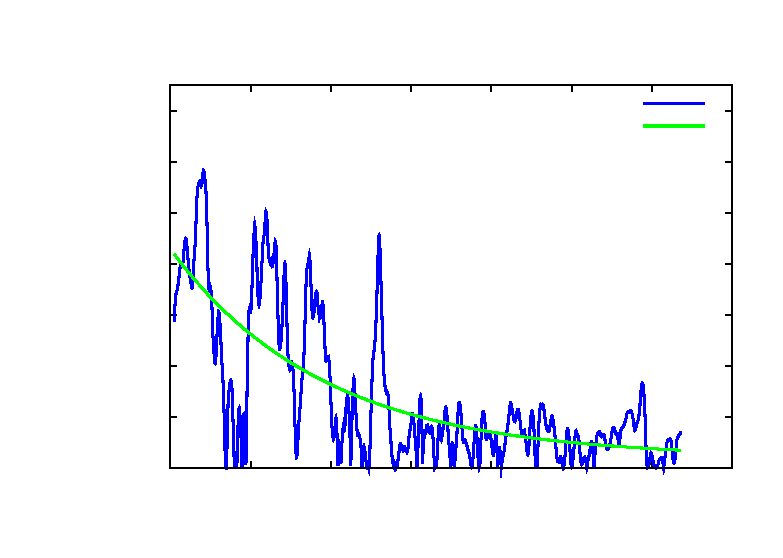
\includegraphics{img/exp1/RL/invJerror_taskHead_1}}%
    \gplfronttext
  \end{picture}%
\endgroup

    }
    \label{fig:exp1:taskHead1:RL}
  }
\caption{Comparison of the fitting for the head task for the \emph{both hands} and \emph{right hand} motion at the second iteration of the identification algorithm.
$r$ are the residues of the optimizations.}
\label{fig:exp1:taskHead1}
\end{figure*}

satan satan satan satan satan satan satan satan satan satan satan
satan satan satan satan satan satan satan satan satan satan satan
satan satan satan satan satan satan satan satan satan satan satan
satan satan satan satan satan satan satan satan satan satan satan
satan satan satan satan satan satan satan satan satan satan satan
satan satan satan satan satan satan satan satan satan satan satan
satan satan satan satan satan satan satan satan satan satan satan

\begin{figure*}[t]
  \centering
  \subfigure[Right hand motion - iteration 1]{
    \resizebox{.48\textwidth}{!} {
      % GNUPLOT: LaTeX picture with Postscript
\begingroup
  \makeatletter
  \providecommand\color[2][]{%
    \GenericError{(gnuplot) \space\space\space\@spaces}{%
      Package color not loaded in conjunction with
      terminal option `colourtext'%
    }{See the gnuplot documentation for explanation.%
    }{Either use 'blacktext' in gnuplot or load the package
      color.sty in LaTeX.}%
    \renewcommand\color[2][]{}%
  }%
  \providecommand\includegraphics[2][]{%
    \GenericError{(gnuplot) \space\space\space\@spaces}{%
      Package graphicx or graphics not loaded%
    }{See the gnuplot documentation for explanation.%
    }{The gnuplot epslatex terminal needs graphicx.sty or graphics.sty.}%
    \renewcommand\includegraphics[2][]{}%
  }%
  \providecommand\rotatebox[2]{#2}%
  \@ifundefined{ifGPcolor}{%
    \newif\ifGPcolor
    \GPcolortrue
  }{}%
  \@ifundefined{ifGPblacktext}{%
    \newif\ifGPblacktext
    \GPblacktexttrue
  }{}%
  % define a \g@addto@macro without @ in the name:
  \let\gplgaddtomacro\g@addto@macro
  % define empty templates for all commands taking text:
  \gdef\gplbacktext{}%
  \gdef\gplfronttext{}%
  \makeatother
  \ifGPblacktext
    % no textcolor at all
    \def\colorrgb#1{}%
    \def\colorgray#1{}%
  \else
    % gray or color?
    \ifGPcolor
      \def\colorrgb#1{\color[rgb]{#1}}%
      \def\colorgray#1{\color[gray]{#1}}%
      \expandafter\def\csname LTw\endcsname{\color{white}}%
      \expandafter\def\csname LTb\endcsname{\color{black}}%
      \expandafter\def\csname LTa\endcsname{\color{black}}%
      \expandafter\def\csname LT0\endcsname{\color[rgb]{1,0,0}}%
      \expandafter\def\csname LT1\endcsname{\color[rgb]{0,1,0}}%
      \expandafter\def\csname LT2\endcsname{\color[rgb]{0,0,1}}%
      \expandafter\def\csname LT3\endcsname{\color[rgb]{1,0,1}}%
      \expandafter\def\csname LT4\endcsname{\color[rgb]{0,1,1}}%
      \expandafter\def\csname LT5\endcsname{\color[rgb]{1,1,0}}%
      \expandafter\def\csname LT6\endcsname{\color[rgb]{0,0,0}}%
      \expandafter\def\csname LT7\endcsname{\color[rgb]{1,0.3,0}}%
      \expandafter\def\csname LT8\endcsname{\color[rgb]{0.5,0.5,0.5}}%
    \else
      % gray
      \def\colorrgb#1{\color{black}}%
      \def\colorgray#1{\color[gray]{#1}}%
      \expandafter\def\csname LTw\endcsname{\color{white}}%
      \expandafter\def\csname LTb\endcsname{\color{black}}%
      \expandafter\def\csname LTa\endcsname{\color{black}}%
      \expandafter\def\csname LT0\endcsname{\color{black}}%
      \expandafter\def\csname LT1\endcsname{\color{black}}%
      \expandafter\def\csname LT2\endcsname{\color{black}}%
      \expandafter\def\csname LT3\endcsname{\color{black}}%
      \expandafter\def\csname LT4\endcsname{\color{black}}%
      \expandafter\def\csname LT5\endcsname{\color{black}}%
      \expandafter\def\csname LT6\endcsname{\color{black}}%
      \expandafter\def\csname LT7\endcsname{\color{black}}%
      \expandafter\def\csname LT8\endcsname{\color{black}}%
    \fi
  \fi
  \setlength{\unitlength}{0.0500bp}%
  \begin{picture}(7200.00,5040.00)%
    \gplgaddtomacro\gplbacktext{%
      \csname LTb\endcsname%
      \put(1210,704){\makebox(0,0)[r]{\strut{} 0}}%
      \put(1210,1229){\makebox(0,0)[r]{\strut{} 0.1}}%
      \put(1210,1754){\makebox(0,0)[r]{\strut{} 0.2}}%
      \put(1210,2279){\makebox(0,0)[r]{\strut{} 0.3}}%
      \put(1210,2805){\makebox(0,0)[r]{\strut{} 0.4}}%
      \put(1210,3330){\makebox(0,0)[r]{\strut{} 0.5}}%
      \put(1210,3855){\makebox(0,0)[r]{\strut{} 0.6}}%
      \put(1210,4380){\makebox(0,0)[r]{\strut{} 0.7}}%
      \put(1342,484){\makebox(0,0){\strut{} 0}}%
      \put(2192,484){\makebox(0,0){\strut{} 2}}%
      \put(3043,484){\makebox(0,0){\strut{} 4}}%
      \put(3893,484){\makebox(0,0){\strut{} 6}}%
      \put(4744,484){\makebox(0,0){\strut{} 8}}%
      \put(5594,484){\makebox(0,0){\strut{} 10}}%
      \put(6445,484){\makebox(0,0){\strut{} 12}}%
      \put(440,2542){\rotatebox{90}{\makebox(0,0){\strut{}$\Vert \dot{q}\Vert$ (rad/s)}}}%
      \put(4106,154){\makebox(0,0){\strut{}$t$ (s)}}%
      \put(4106,4710){\makebox(0,0){\strut{}$\begin{array}{rl} r &= 2.94667\\ \int \Vert J^+ \dot{e}_{lhand} \Vert \mathrm{d}t &=  0.167428 \mathrm{rad}\\ \end{array}$}}%
    }%
    \gplgaddtomacro\gplfronttext{%
      \csname LTb\endcsname%
      \put(5883,4207){\makebox(0,0)[r]{\strut{}$J^+ \dot{e}_{lhand} / \int \Vert J^+ \dot{e}_{lhand} \Vert \mathrm{d}t$}}%
      \csname LTb\endcsname%
      \put(5883,3987){\makebox(0,0)[r]{\strut{}Model}}%
    }%
    \gplbacktext
    \put(0,0){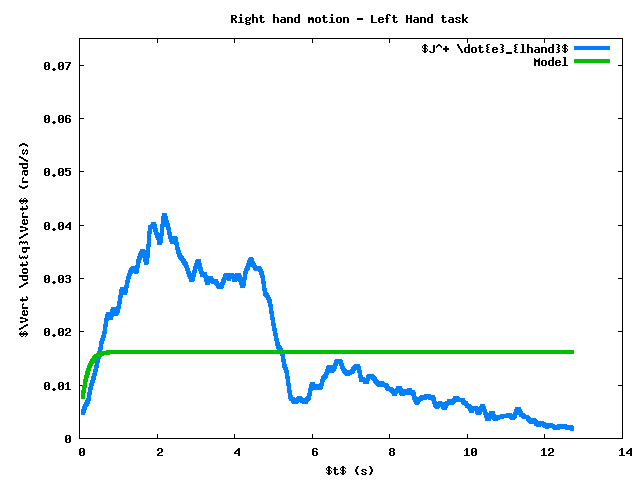
\includegraphics{img/exp1/R/invJerror_taskLhand_1}}%
    \gplfronttext
  \end{picture}%
\endgroup

    }
    \label{fig:exp1:taskLhand1:R}
  }
  \subfigure[Both hands motion - iteration 1]{
    \resizebox{.48\textwidth}{!} {
      % GNUPLOT: LaTeX picture with Postscript
\begingroup
  \makeatletter
  \providecommand\color[2][]{%
    \GenericError{(gnuplot) \space\space\space\@spaces}{%
      Package color not loaded in conjunction with
      terminal option `colourtext'%
    }{See the gnuplot documentation for explanation.%
    }{Either use 'blacktext' in gnuplot or load the package
      color.sty in LaTeX.}%
    \renewcommand\color[2][]{}%
  }%
  \providecommand\includegraphics[2][]{%
    \GenericError{(gnuplot) \space\space\space\@spaces}{%
      Package graphicx or graphics not loaded%
    }{See the gnuplot documentation for explanation.%
    }{The gnuplot epslatex terminal needs graphicx.sty or graphics.sty.}%
    \renewcommand\includegraphics[2][]{}%
  }%
  \providecommand\rotatebox[2]{#2}%
  \@ifundefined{ifGPcolor}{%
    \newif\ifGPcolor
    \GPcolortrue
  }{}%
  \@ifundefined{ifGPblacktext}{%
    \newif\ifGPblacktext
    \GPblacktexttrue
  }{}%
  % define a \g@addto@macro without @ in the name:
  \let\gplgaddtomacro\g@addto@macro
  % define empty templates for all commands taking text:
  \gdef\gplbacktext{}%
  \gdef\gplfronttext{}%
  \makeatother
  \ifGPblacktext
    % no textcolor at all
    \def\colorrgb#1{}%
    \def\colorgray#1{}%
  \else
    % gray or color?
    \ifGPcolor
      \def\colorrgb#1{\color[rgb]{#1}}%
      \def\colorgray#1{\color[gray]{#1}}%
      \expandafter\def\csname LTw\endcsname{\color{white}}%
      \expandafter\def\csname LTb\endcsname{\color{black}}%
      \expandafter\def\csname LTa\endcsname{\color{black}}%
      \expandafter\def\csname LT0\endcsname{\color[rgb]{1,0,0}}%
      \expandafter\def\csname LT1\endcsname{\color[rgb]{0,1,0}}%
      \expandafter\def\csname LT2\endcsname{\color[rgb]{0,0,1}}%
      \expandafter\def\csname LT3\endcsname{\color[rgb]{1,0,1}}%
      \expandafter\def\csname LT4\endcsname{\color[rgb]{0,1,1}}%
      \expandafter\def\csname LT5\endcsname{\color[rgb]{1,1,0}}%
      \expandafter\def\csname LT6\endcsname{\color[rgb]{0,0,0}}%
      \expandafter\def\csname LT7\endcsname{\color[rgb]{1,0.3,0}}%
      \expandafter\def\csname LT8\endcsname{\color[rgb]{0.5,0.5,0.5}}%
    \else
      % gray
      \def\colorrgb#1{\color{black}}%
      \def\colorgray#1{\color[gray]{#1}}%
      \expandafter\def\csname LTw\endcsname{\color{white}}%
      \expandafter\def\csname LTb\endcsname{\color{black}}%
      \expandafter\def\csname LTa\endcsname{\color{black}}%
      \expandafter\def\csname LT0\endcsname{\color{black}}%
      \expandafter\def\csname LT1\endcsname{\color{black}}%
      \expandafter\def\csname LT2\endcsname{\color{black}}%
      \expandafter\def\csname LT3\endcsname{\color{black}}%
      \expandafter\def\csname LT4\endcsname{\color{black}}%
      \expandafter\def\csname LT5\endcsname{\color{black}}%
      \expandafter\def\csname LT6\endcsname{\color{black}}%
      \expandafter\def\csname LT7\endcsname{\color{black}}%
      \expandafter\def\csname LT8\endcsname{\color{black}}%
    \fi
  \fi
  \setlength{\unitlength}{0.0500bp}%
  \begin{picture}(7200.00,5040.00)%
    \gplgaddtomacro\gplbacktext{%
      \csname LTb\endcsname%
      \put(1342,704){\makebox(0,0)[r]{\strut{} 0}}%
      \put(1342,1194){\makebox(0,0)[r]{\strut{} 0.01}}%
      \put(1342,1684){\makebox(0,0)[r]{\strut{} 0.02}}%
      \put(1342,2174){\makebox(0,0)[r]{\strut{} 0.03}}%
      \put(1342,2665){\makebox(0,0)[r]{\strut{} 0.04}}%
      \put(1342,3155){\makebox(0,0)[r]{\strut{} 0.05}}%
      \put(1342,3645){\makebox(0,0)[r]{\strut{} 0.06}}%
      \put(1342,4135){\makebox(0,0)[r]{\strut{} 0.07}}%
      \put(1474,484){\makebox(0,0){\strut{} 0}}%
      \put(2245,484){\makebox(0,0){\strut{} 2}}%
      \put(3016,484){\makebox(0,0){\strut{} 4}}%
      \put(3787,484){\makebox(0,0){\strut{} 6}}%
      \put(4557,484){\makebox(0,0){\strut{} 8}}%
      \put(5328,484){\makebox(0,0){\strut{} 10}}%
      \put(6099,484){\makebox(0,0){\strut{} 12}}%
      \put(6870,484){\makebox(0,0){\strut{} 14}}%
      \put(440,2542){\rotatebox{90}{\makebox(0,0){\strut{}$\Vert \dot{q}\Vert$ (rad/s)}}}%
      \put(4172,154){\makebox(0,0){\strut{}$t$ (s)}}%
      \put(4172,4710){\makebox(0,0){\strut{}Right and left hand motion - Left hand task}}%
    }%
    \gplgaddtomacro\gplfronttext{%
      \csname LTb\endcsname%
      \put(5883,4207){\makebox(0,0)[r]{\strut{}$J^+ \dot{e}_{lhand}$}}%
      \csname LTb\endcsname%
      \put(5883,3987){\makebox(0,0)[r]{\strut{}Model}}%
    }%
    \gplbacktext
    \put(0,0){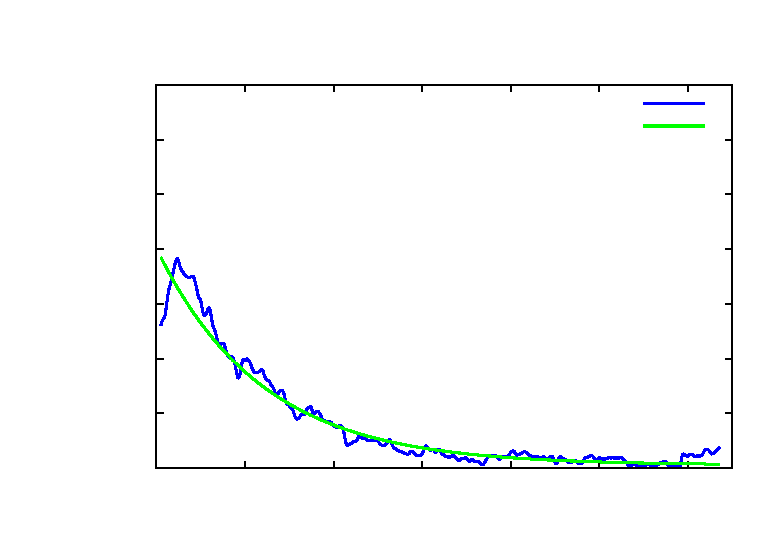
\includegraphics{img/exp1/RL/invJerror_taskLhand_1}}%
    \gplfronttext
  \end{picture}%
\endgroup

    }
    \label{fig:exp1:taskLhand1:RL}
  }
  \caption{Comparison of the fitting for the left hand task for the
    \emph{both hands} and \emph{right hand} motion at the second
    iteration of the identification algorithm.  $r$ are
    the residues of the optimizations.}
  \label{fig:exp1:taskLhand1}
\end{figure*}

satan satan satan satan satan satan satan satan satan satan satan
satan satan satan satan satan satan satan satan satan satan satan
satan satan satan satan satan satan satan satan satan satan satan
satan satan satan satan satan satan satan satan satan satan satan
satan satan satan satan satan satan satan satan satan satan satan
satan satan satan satan satan satan satan satan satan satan satan
satan satan satan satan satan satan satan satan satan satan satan
satan satan satan satan satan satan satan satan satan satan satan
satan satan satan satan satan satan satan satan satan satan satan

\begin{figure*}[t]
  \centering
  \subfigure[Right hand motion - iteration 1]{
  \resizebox{.48\textwidth}{!} {
	% GNUPLOT: LaTeX picture with Postscript
\begingroup
  \makeatletter
  \providecommand\color[2][]{%
    \GenericError{(gnuplot) \space\space\space\@spaces}{%
      Package color not loaded in conjunction with
      terminal option `colourtext'%
    }{See the gnuplot documentation for explanation.%
    }{Either use 'blacktext' in gnuplot or load the package
      color.sty in LaTeX.}%
    \renewcommand\color[2][]{}%
  }%
  \providecommand\includegraphics[2][]{%
    \GenericError{(gnuplot) \space\space\space\@spaces}{%
      Package graphicx or graphics not loaded%
    }{See the gnuplot documentation for explanation.%
    }{The gnuplot epslatex terminal needs graphicx.sty or graphics.sty.}%
    \renewcommand\includegraphics[2][]{}%
  }%
  \providecommand\rotatebox[2]{#2}%
  \@ifundefined{ifGPcolor}{%
    \newif\ifGPcolor
    \GPcolortrue
  }{}%
  \@ifundefined{ifGPblacktext}{%
    \newif\ifGPblacktext
    \GPblacktexttrue
  }{}%
  % define a \g@addto@macro without @ in the name:
  \let\gplgaddtomacro\g@addto@macro
  % define empty templates for all commands taking text:
  \gdef\gplbacktext{}%
  \gdef\gplfronttext{}%
  \makeatother
  \ifGPblacktext
    % no textcolor at all
    \def\colorrgb#1{}%
    \def\colorgray#1{}%
  \else
    % gray or color?
    \ifGPcolor
      \def\colorrgb#1{\color[rgb]{#1}}%
      \def\colorgray#1{\color[gray]{#1}}%
      \expandafter\def\csname LTw\endcsname{\color{white}}%
      \expandafter\def\csname LTb\endcsname{\color{black}}%
      \expandafter\def\csname LTa\endcsname{\color{black}}%
      \expandafter\def\csname LT0\endcsname{\color[rgb]{1,0,0}}%
      \expandafter\def\csname LT1\endcsname{\color[rgb]{0,1,0}}%
      \expandafter\def\csname LT2\endcsname{\color[rgb]{0,0,1}}%
      \expandafter\def\csname LT3\endcsname{\color[rgb]{1,0,1}}%
      \expandafter\def\csname LT4\endcsname{\color[rgb]{0,1,1}}%
      \expandafter\def\csname LT5\endcsname{\color[rgb]{1,1,0}}%
      \expandafter\def\csname LT6\endcsname{\color[rgb]{0,0,0}}%
      \expandafter\def\csname LT7\endcsname{\color[rgb]{1,0.3,0}}%
      \expandafter\def\csname LT8\endcsname{\color[rgb]{0.5,0.5,0.5}}%
    \else
      % gray
      \def\colorrgb#1{\color{black}}%
      \def\colorgray#1{\color[gray]{#1}}%
      \expandafter\def\csname LTw\endcsname{\color{white}}%
      \expandafter\def\csname LTb\endcsname{\color{black}}%
      \expandafter\def\csname LTa\endcsname{\color{black}}%
      \expandafter\def\csname LT0\endcsname{\color{black}}%
      \expandafter\def\csname LT1\endcsname{\color{black}}%
      \expandafter\def\csname LT2\endcsname{\color{black}}%
      \expandafter\def\csname LT3\endcsname{\color{black}}%
      \expandafter\def\csname LT4\endcsname{\color{black}}%
      \expandafter\def\csname LT5\endcsname{\color{black}}%
      \expandafter\def\csname LT6\endcsname{\color{black}}%
      \expandafter\def\csname LT7\endcsname{\color{black}}%
      \expandafter\def\csname LT8\endcsname{\color{black}}%
    \fi
  \fi
  \setlength{\unitlength}{0.0500bp}%
  \begin{picture}(7200.00,5040.00)%
    \gplgaddtomacro\gplbacktext{%
      \csname LTb\endcsname%
      \put(1210,704){\makebox(0,0)[r]{\strut{} 0}}%
      \put(1210,1229){\makebox(0,0)[r]{\strut{} 0.1}}%
      \put(1210,1754){\makebox(0,0)[r]{\strut{} 0.2}}%
      \put(1210,2279){\makebox(0,0)[r]{\strut{} 0.3}}%
      \put(1210,2805){\makebox(0,0)[r]{\strut{} 0.4}}%
      \put(1210,3330){\makebox(0,0)[r]{\strut{} 0.5}}%
      \put(1210,3855){\makebox(0,0)[r]{\strut{} 0.6}}%
      \put(1210,4380){\makebox(0,0)[r]{\strut{} 0.7}}%
      \put(1342,484){\makebox(0,0){\strut{} 0}}%
      \put(2192,484){\makebox(0,0){\strut{} 2}}%
      \put(3043,484){\makebox(0,0){\strut{} 4}}%
      \put(3893,484){\makebox(0,0){\strut{} 6}}%
      \put(4744,484){\makebox(0,0){\strut{} 8}}%
      \put(5594,484){\makebox(0,0){\strut{} 10}}%
      \put(6445,484){\makebox(0,0){\strut{} 12}}%
      \put(440,2542){\rotatebox{90}{\makebox(0,0){\strut{}$\Vert \dot{q}\Vert$ (rad/s)}}}%
      \put(4106,154){\makebox(0,0){\strut{}$t$ (s)}}%
      \put(4106,4710){\makebox(0,0){\strut{}$\begin{array}{rl} r &= 0.788495\\ \int \Vert J^+ \dot{e}_{twofeet} \Vert \mathrm{d}t &=  0.254531 \mathrm{rad}\\ \end{array}$}}%
    }%
    \gplgaddtomacro\gplfronttext{%
      \csname LTb\endcsname%
      \put(5883,4207){\makebox(0,0)[r]{\strut{}$J^+ \dot{e}_{twofeet} / \int \Vert J^+ \dot{e}_{twofeet} \Vert \mathrm{d}t$}}%
      \csname LTb\endcsname%
      \put(5883,3987){\makebox(0,0)[r]{\strut{}Model}}%
    }%
    \gplbacktext
    \put(0,0){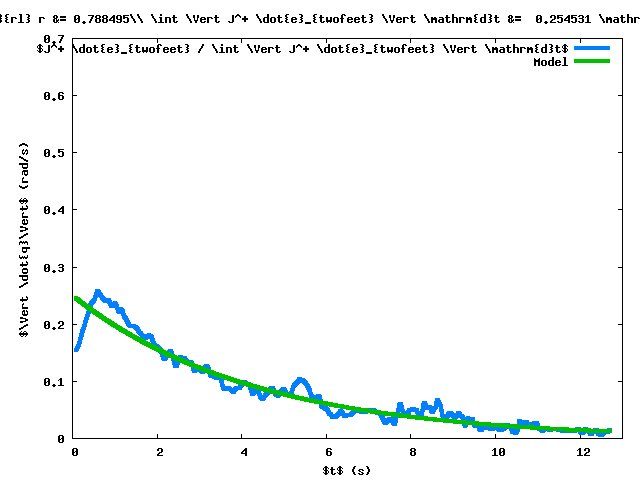
\includegraphics{img/exp1/R/invJerror_taskTwofeet_1}}%
    \gplfronttext
  \end{picture}%
\endgroup

    }
    \label{fig:exp1:taskTwofeet1:R}
  }
  \subfigure[Both hands motion - iteration 1]{
  \resizebox{.48\textwidth}{!} {
	% GNUPLOT: LaTeX picture with Postscript
\begingroup
  \makeatletter
  \providecommand\color[2][]{%
    \GenericError{(gnuplot) \space\space\space\@spaces}{%
      Package color not loaded in conjunction with
      terminal option `colourtext'%
    }{See the gnuplot documentation for explanation.%
    }{Either use 'blacktext' in gnuplot or load the package
      color.sty in LaTeX.}%
    \renewcommand\color[2][]{}%
  }%
  \providecommand\includegraphics[2][]{%
    \GenericError{(gnuplot) \space\space\space\@spaces}{%
      Package graphicx or graphics not loaded%
    }{See the gnuplot documentation for explanation.%
    }{The gnuplot epslatex terminal needs graphicx.sty or graphics.sty.}%
    \renewcommand\includegraphics[2][]{}%
  }%
  \providecommand\rotatebox[2]{#2}%
  \@ifundefined{ifGPcolor}{%
    \newif\ifGPcolor
    \GPcolortrue
  }{}%
  \@ifundefined{ifGPblacktext}{%
    \newif\ifGPblacktext
    \GPblacktexttrue
  }{}%
  % define a \g@addto@macro without @ in the name:
  \let\gplgaddtomacro\g@addto@macro
  % define empty templates for all commands taking text:
  \gdef\gplbacktext{}%
  \gdef\gplfronttext{}%
  \makeatother
  \ifGPblacktext
    % no textcolor at all
    \def\colorrgb#1{}%
    \def\colorgray#1{}%
  \else
    % gray or color?
    \ifGPcolor
      \def\colorrgb#1{\color[rgb]{#1}}%
      \def\colorgray#1{\color[gray]{#1}}%
      \expandafter\def\csname LTw\endcsname{\color{white}}%
      \expandafter\def\csname LTb\endcsname{\color{black}}%
      \expandafter\def\csname LTa\endcsname{\color{black}}%
      \expandafter\def\csname LT0\endcsname{\color[rgb]{1,0,0}}%
      \expandafter\def\csname LT1\endcsname{\color[rgb]{0,1,0}}%
      \expandafter\def\csname LT2\endcsname{\color[rgb]{0,0,1}}%
      \expandafter\def\csname LT3\endcsname{\color[rgb]{1,0,1}}%
      \expandafter\def\csname LT4\endcsname{\color[rgb]{0,1,1}}%
      \expandafter\def\csname LT5\endcsname{\color[rgb]{1,1,0}}%
      \expandafter\def\csname LT6\endcsname{\color[rgb]{0,0,0}}%
      \expandafter\def\csname LT7\endcsname{\color[rgb]{1,0.3,0}}%
      \expandafter\def\csname LT8\endcsname{\color[rgb]{0.5,0.5,0.5}}%
    \else
      % gray
      \def\colorrgb#1{\color{black}}%
      \def\colorgray#1{\color[gray]{#1}}%
      \expandafter\def\csname LTw\endcsname{\color{white}}%
      \expandafter\def\csname LTb\endcsname{\color{black}}%
      \expandafter\def\csname LTa\endcsname{\color{black}}%
      \expandafter\def\csname LT0\endcsname{\color{black}}%
      \expandafter\def\csname LT1\endcsname{\color{black}}%
      \expandafter\def\csname LT2\endcsname{\color{black}}%
      \expandafter\def\csname LT3\endcsname{\color{black}}%
      \expandafter\def\csname LT4\endcsname{\color{black}}%
      \expandafter\def\csname LT5\endcsname{\color{black}}%
      \expandafter\def\csname LT6\endcsname{\color{black}}%
      \expandafter\def\csname LT7\endcsname{\color{black}}%
      \expandafter\def\csname LT8\endcsname{\color{black}}%
    \fi
  \fi
  \setlength{\unitlength}{0.0500bp}%
  \begin{picture}(7200.00,5040.00)%
    \gplgaddtomacro\gplbacktext{%
      \csname LTb\endcsname%
      \put(1342,704){\makebox(0,0)[r]{\strut{} 0}}%
      \put(1342,1194){\makebox(0,0)[r]{\strut{} 0.01}}%
      \put(1342,1684){\makebox(0,0)[r]{\strut{} 0.02}}%
      \put(1342,2174){\makebox(0,0)[r]{\strut{} 0.03}}%
      \put(1342,2665){\makebox(0,0)[r]{\strut{} 0.04}}%
      \put(1342,3155){\makebox(0,0)[r]{\strut{} 0.05}}%
      \put(1342,3645){\makebox(0,0)[r]{\strut{} 0.06}}%
      \put(1342,4135){\makebox(0,0)[r]{\strut{} 0.07}}%
      \put(1474,484){\makebox(0,0){\strut{} 0}}%
      \put(2245,484){\makebox(0,0){\strut{} 2}}%
      \put(3016,484){\makebox(0,0){\strut{} 4}}%
      \put(3787,484){\makebox(0,0){\strut{} 6}}%
      \put(4557,484){\makebox(0,0){\strut{} 8}}%
      \put(5328,484){\makebox(0,0){\strut{} 10}}%
      \put(6099,484){\makebox(0,0){\strut{} 12}}%
      \put(6870,484){\makebox(0,0){\strut{} 14}}%
      \put(440,2542){\rotatebox{90}{\makebox(0,0){\strut{}$\Vert \dot{q}\Vert$ (rad/s)}}}%
      \put(4172,154){\makebox(0,0){\strut{}$t$ (s)}}%
      \put(4172,4710){\makebox(0,0){\strut{}Right and left hand motion - Twofeet task}}%
    }%
    \gplgaddtomacro\gplfronttext{%
      \csname LTb\endcsname%
      \put(5883,4207){\makebox(0,0)[r]{\strut{}$J^+ \dot{e}_{twofeet}$}}%
      \csname LTb\endcsname%
      \put(5883,3987){\makebox(0,0)[r]{\strut{}Model}}%
    }%
    \gplbacktext
    \put(0,0){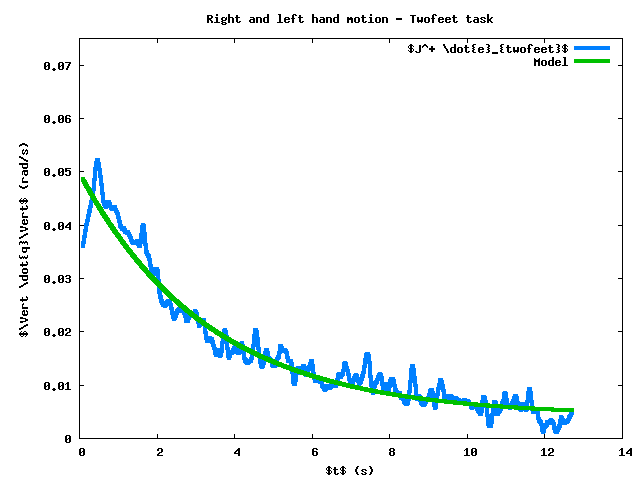
\includegraphics{img/exp1/RL/invJerror_taskTwofeet_1}}%
    \gplfronttext
  \end{picture}%
\endgroup

    }
    \label{fig:exp1:taskTwofeet1:RL}
  }
\caption{Comparison of the fitting for the \emph{two feet} task for the \emph{both hands} and \emph{right hand} motion at the second iteration of the identification algorithm. $r$ are the residues of the optimizations.}
\label{fig:exp1:taskTwofeet1}
\end{figure*}

%%%%%%%%%%%%%%%%%%%%%%%%%%%%%%%%%%%%%%%%%
satan satan satan satan satan satan satan satan satan satan satan
satan satan satan satan satan satan satan satan satan satan satan
satan satan satan satan satan satan satan satan satan satan satan
satan satan satan satan satan satan satan satan satan satan satan
satan satan satan satan satan satan satan satan satan satan satan

\begin{figure*}[t]
  \centering
  \subfigure[Right hand motion - iteration 2]{
  \resizebox{.48\textwidth}{!} {
	% GNUPLOT: LaTeX picture with Postscript
\begingroup
  \makeatletter
  \providecommand\color[2][]{%
    \GenericError{(gnuplot) \space\space\space\@spaces}{%
      Package color not loaded in conjunction with
      terminal option `colourtext'%
    }{See the gnuplot documentation for explanation.%
    }{Either use 'blacktext' in gnuplot or load the package
      color.sty in LaTeX.}%
    \renewcommand\color[2][]{}%
  }%
  \providecommand\includegraphics[2][]{%
    \GenericError{(gnuplot) \space\space\space\@spaces}{%
      Package graphicx or graphics not loaded%
    }{See the gnuplot documentation for explanation.%
    }{The gnuplot epslatex terminal needs graphicx.sty or graphics.sty.}%
    \renewcommand\includegraphics[2][]{}%
  }%
  \providecommand\rotatebox[2]{#2}%
  \@ifundefined{ifGPcolor}{%
    \newif\ifGPcolor
    \GPcolortrue
  }{}%
  \@ifundefined{ifGPblacktext}{%
    \newif\ifGPblacktext
    \GPblacktexttrue
  }{}%
  % define a \g@addto@macro without @ in the name:
  \let\gplgaddtomacro\g@addto@macro
  % define empty templates for all commands taking text:
  \gdef\gplbacktext{}%
  \gdef\gplfronttext{}%
  \makeatother
  \ifGPblacktext
    % no textcolor at all
    \def\colorrgb#1{}%
    \def\colorgray#1{}%
  \else
    % gray or color?
    \ifGPcolor
      \def\colorrgb#1{\color[rgb]{#1}}%
      \def\colorgray#1{\color[gray]{#1}}%
      \expandafter\def\csname LTw\endcsname{\color{white}}%
      \expandafter\def\csname LTb\endcsname{\color{black}}%
      \expandafter\def\csname LTa\endcsname{\color{black}}%
      \expandafter\def\csname LT0\endcsname{\color[rgb]{1,0,0}}%
      \expandafter\def\csname LT1\endcsname{\color[rgb]{0,1,0}}%
      \expandafter\def\csname LT2\endcsname{\color[rgb]{0,0,1}}%
      \expandafter\def\csname LT3\endcsname{\color[rgb]{1,0,1}}%
      \expandafter\def\csname LT4\endcsname{\color[rgb]{0,1,1}}%
      \expandafter\def\csname LT5\endcsname{\color[rgb]{1,1,0}}%
      \expandafter\def\csname LT6\endcsname{\color[rgb]{0,0,0}}%
      \expandafter\def\csname LT7\endcsname{\color[rgb]{1,0.3,0}}%
      \expandafter\def\csname LT8\endcsname{\color[rgb]{0.5,0.5,0.5}}%
    \else
      % gray
      \def\colorrgb#1{\color{black}}%
      \def\colorgray#1{\color[gray]{#1}}%
      \expandafter\def\csname LTw\endcsname{\color{white}}%
      \expandafter\def\csname LTb\endcsname{\color{black}}%
      \expandafter\def\csname LTa\endcsname{\color{black}}%
      \expandafter\def\csname LT0\endcsname{\color{black}}%
      \expandafter\def\csname LT1\endcsname{\color{black}}%
      \expandafter\def\csname LT2\endcsname{\color{black}}%
      \expandafter\def\csname LT3\endcsname{\color{black}}%
      \expandafter\def\csname LT4\endcsname{\color{black}}%
      \expandafter\def\csname LT5\endcsname{\color{black}}%
      \expandafter\def\csname LT6\endcsname{\color{black}}%
      \expandafter\def\csname LT7\endcsname{\color{black}}%
      \expandafter\def\csname LT8\endcsname{\color{black}}%
    \fi
  \fi
  \setlength{\unitlength}{0.0500bp}%
  \begin{picture}(7200.00,5040.00)%
    \gplgaddtomacro\gplbacktext{%
      \csname LTb\endcsname%
      \put(1342,704){\makebox(0,0)[r]{\strut{} 0}}%
      \put(1342,1194){\makebox(0,0)[r]{\strut{} 0.01}}%
      \put(1342,1684){\makebox(0,0)[r]{\strut{} 0.02}}%
      \put(1342,2174){\makebox(0,0)[r]{\strut{} 0.03}}%
      \put(1342,2665){\makebox(0,0)[r]{\strut{} 0.04}}%
      \put(1342,3155){\makebox(0,0)[r]{\strut{} 0.05}}%
      \put(1342,3645){\makebox(0,0)[r]{\strut{} 0.06}}%
      \put(1342,4135){\makebox(0,0)[r]{\strut{} 0.07}}%
      \put(1474,484){\makebox(0,0){\strut{} 0}}%
      \put(2245,484){\makebox(0,0){\strut{} 2}}%
      \put(3016,484){\makebox(0,0){\strut{} 4}}%
      \put(3787,484){\makebox(0,0){\strut{} 6}}%
      \put(4557,484){\makebox(0,0){\strut{} 8}}%
      \put(5328,484){\makebox(0,0){\strut{} 10}}%
      \put(6099,484){\makebox(0,0){\strut{} 12}}%
      \put(6870,484){\makebox(0,0){\strut{} 14}}%
      \put(440,2542){\rotatebox{90}{\makebox(0,0){\strut{}$\Vert \dot{q}\Vert$ (rad/s)}}}%
      \put(4172,154){\makebox(0,0){\strut{}$t$ (s)}}%
      \put(4172,4710){\makebox(0,0){\strut{}Right hand motion - Head task}}%
    }%
    \gplgaddtomacro\gplfronttext{%
      \csname LTb\endcsname%
      \put(5883,4207){\makebox(0,0)[r]{\strut{}$J^+ \dot{e}_{head}$}}%
      \csname LTb\endcsname%
      \put(5883,3987){\makebox(0,0)[r]{\strut{}Model}}%
    }%
    \gplbacktext
    \put(0,0){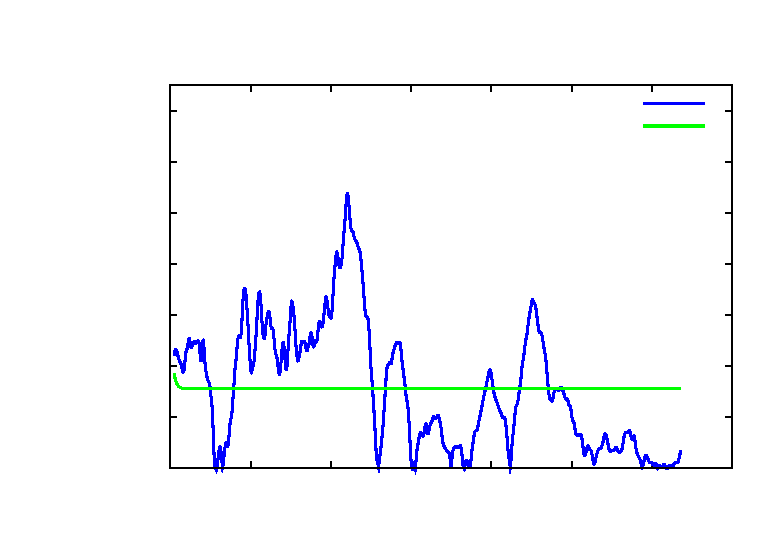
\includegraphics{img/exp1/R/invJerror_taskHead_2}}%
    \gplfronttext
  \end{picture}%
\endgroup

    } 
    \label{fig:exp1:taskHead2:R}
  }
  \subfigure[Both hands motion - iteration 2]{
  \resizebox{.48\textwidth}{!} {
	% GNUPLOT: LaTeX picture with Postscript
\begingroup
  \makeatletter
  \providecommand\color[2][]{%
    \GenericError{(gnuplot) \space\space\space\@spaces}{%
      Package color not loaded in conjunction with
      terminal option `colourtext'%
    }{See the gnuplot documentation for explanation.%
    }{Either use 'blacktext' in gnuplot or load the package
      color.sty in LaTeX.}%
    \renewcommand\color[2][]{}%
  }%
  \providecommand\includegraphics[2][]{%
    \GenericError{(gnuplot) \space\space\space\@spaces}{%
      Package graphicx or graphics not loaded%
    }{See the gnuplot documentation for explanation.%
    }{The gnuplot epslatex terminal needs graphicx.sty or graphics.sty.}%
    \renewcommand\includegraphics[2][]{}%
  }%
  \providecommand\rotatebox[2]{#2}%
  \@ifundefined{ifGPcolor}{%
    \newif\ifGPcolor
    \GPcolortrue
  }{}%
  \@ifundefined{ifGPblacktext}{%
    \newif\ifGPblacktext
    \GPblacktexttrue
  }{}%
  % define a \g@addto@macro without @ in the name:
  \let\gplgaddtomacro\g@addto@macro
  % define empty templates for all commands taking text:
  \gdef\gplbacktext{}%
  \gdef\gplfronttext{}%
  \makeatother
  \ifGPblacktext
    % no textcolor at all
    \def\colorrgb#1{}%
    \def\colorgray#1{}%
  \else
    % gray or color?
    \ifGPcolor
      \def\colorrgb#1{\color[rgb]{#1}}%
      \def\colorgray#1{\color[gray]{#1}}%
      \expandafter\def\csname LTw\endcsname{\color{white}}%
      \expandafter\def\csname LTb\endcsname{\color{black}}%
      \expandafter\def\csname LTa\endcsname{\color{black}}%
      \expandafter\def\csname LT0\endcsname{\color[rgb]{1,0,0}}%
      \expandafter\def\csname LT1\endcsname{\color[rgb]{0,1,0}}%
      \expandafter\def\csname LT2\endcsname{\color[rgb]{0,0,1}}%
      \expandafter\def\csname LT3\endcsname{\color[rgb]{1,0,1}}%
      \expandafter\def\csname LT4\endcsname{\color[rgb]{0,1,1}}%
      \expandafter\def\csname LT5\endcsname{\color[rgb]{1,1,0}}%
      \expandafter\def\csname LT6\endcsname{\color[rgb]{0,0,0}}%
      \expandafter\def\csname LT7\endcsname{\color[rgb]{1,0.3,0}}%
      \expandafter\def\csname LT8\endcsname{\color[rgb]{0.5,0.5,0.5}}%
    \else
      % gray
      \def\colorrgb#1{\color{black}}%
      \def\colorgray#1{\color[gray]{#1}}%
      \expandafter\def\csname LTw\endcsname{\color{white}}%
      \expandafter\def\csname LTb\endcsname{\color{black}}%
      \expandafter\def\csname LTa\endcsname{\color{black}}%
      \expandafter\def\csname LT0\endcsname{\color{black}}%
      \expandafter\def\csname LT1\endcsname{\color{black}}%
      \expandafter\def\csname LT2\endcsname{\color{black}}%
      \expandafter\def\csname LT3\endcsname{\color{black}}%
      \expandafter\def\csname LT4\endcsname{\color{black}}%
      \expandafter\def\csname LT5\endcsname{\color{black}}%
      \expandafter\def\csname LT6\endcsname{\color{black}}%
      \expandafter\def\csname LT7\endcsname{\color{black}}%
      \expandafter\def\csname LT8\endcsname{\color{black}}%
    \fi
  \fi
  \setlength{\unitlength}{0.0500bp}%
  \begin{picture}(7200.00,5040.00)%
    \gplgaddtomacro\gplbacktext{%
      \csname LTb\endcsname%
      \put(1210,704){\makebox(0,0)[r]{\strut{} 0}}%
      \put(1210,1229){\makebox(0,0)[r]{\strut{} 0.1}}%
      \put(1210,1754){\makebox(0,0)[r]{\strut{} 0.2}}%
      \put(1210,2279){\makebox(0,0)[r]{\strut{} 0.3}}%
      \put(1210,2805){\makebox(0,0)[r]{\strut{} 0.4}}%
      \put(1210,3330){\makebox(0,0)[r]{\strut{} 0.5}}%
      \put(1210,3855){\makebox(0,0)[r]{\strut{} 0.6}}%
      \put(1210,4380){\makebox(0,0)[r]{\strut{} 0.7}}%
      \put(1342,484){\makebox(0,0){\strut{} 0}}%
      \put(2192,484){\makebox(0,0){\strut{} 2}}%
      \put(3043,484){\makebox(0,0){\strut{} 4}}%
      \put(3893,484){\makebox(0,0){\strut{} 6}}%
      \put(4744,484){\makebox(0,0){\strut{} 8}}%
      \put(5594,484){\makebox(0,0){\strut{} 10}}%
      \put(6445,484){\makebox(0,0){\strut{} 12}}%
      \put(440,2542){\rotatebox{90}{\makebox(0,0){\strut{}$\Vert \dot{q}\Vert$ (rad/s)}}}%
      \put(4106,154){\makebox(0,0){\strut{}$t$ (s)}}%
      \put(4106,4710){\makebox(0,0){\strut{}$\begin{array}{rl} r &= 2.01932\\ \int \Vert J^+ \dot{e}_{head} \Vert \mathrm{d}t &=  0.0256238 \mathrm{rad}\\ \end{array}$}}%
    }%
    \gplgaddtomacro\gplfronttext{%
      \csname LTb\endcsname%
      \put(5883,4207){\makebox(0,0)[r]{\strut{}$J^+ \dot{e}_{head} / \int \Vert J^+ \dot{e}_{head} \Vert \mathrm{d}t$}}%
      \csname LTb\endcsname%
      \put(5883,3987){\makebox(0,0)[r]{\strut{}Model}}%
    }%
    \gplbacktext
    \put(0,0){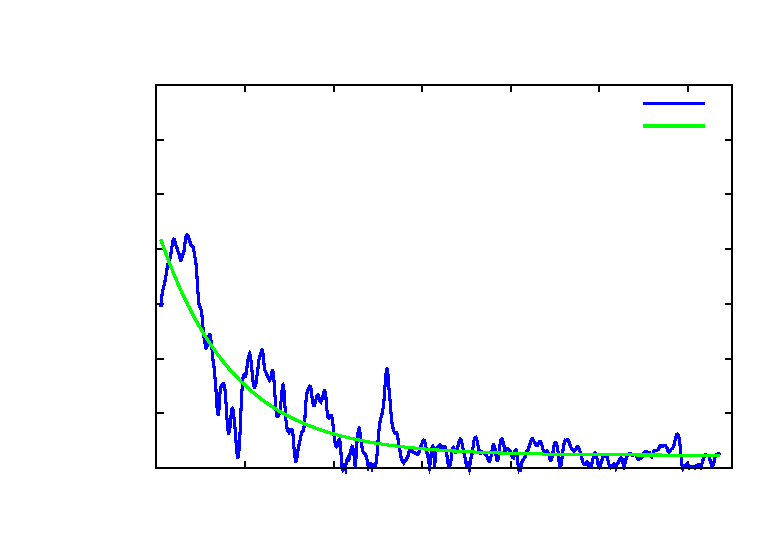
\includegraphics{img/exp1/RL/invJerror_taskHead_2}}%
    \gplfronttext
  \end{picture}%
\endgroup

    }
    \label{fig:exp1:taskHead2:RL}
  }
\caption{Comparison of the fitting for the head task for the \emph{both hands} and \emph{right hand} motion at the third iteration of the identification algorithm.
$r$ are the residues of the optimizations.}
\label{fig:exp1:taskHead2}
\end{figure*}

satan satan satan satan satan satan satan satan satan satan satan
satan satan satan satan satan satan satan satan satan satan satan
satan satan satan satan satan satan satan satan satan satan satan
satan satan satan satan satan satan satan satan satan satan satan
satan satan satan satan satan satan satan satan satan satan satan
satan satan satan satan satan satan satan satan satan satan satan
satan

\begin{figure*}[t]
  \centering
  \subfigure[Right hand motion - iteration 2]{
  \resizebox{.48\textwidth}{!} {
	% GNUPLOT: LaTeX picture with Postscript
\begingroup
  \makeatletter
  \providecommand\color[2][]{%
    \GenericError{(gnuplot) \space\space\space\@spaces}{%
      Package color not loaded in conjunction with
      terminal option `colourtext'%
    }{See the gnuplot documentation for explanation.%
    }{Either use 'blacktext' in gnuplot or load the package
      color.sty in LaTeX.}%
    \renewcommand\color[2][]{}%
  }%
  \providecommand\includegraphics[2][]{%
    \GenericError{(gnuplot) \space\space\space\@spaces}{%
      Package graphicx or graphics not loaded%
    }{See the gnuplot documentation for explanation.%
    }{The gnuplot epslatex terminal needs graphicx.sty or graphics.sty.}%
    \renewcommand\includegraphics[2][]{}%
  }%
  \providecommand\rotatebox[2]{#2}%
  \@ifundefined{ifGPcolor}{%
    \newif\ifGPcolor
    \GPcolortrue
  }{}%
  \@ifundefined{ifGPblacktext}{%
    \newif\ifGPblacktext
    \GPblacktexttrue
  }{}%
  % define a \g@addto@macro without @ in the name:
  \let\gplgaddtomacro\g@addto@macro
  % define empty templates for all commands taking text:
  \gdef\gplbacktext{}%
  \gdef\gplfronttext{}%
  \makeatother
  \ifGPblacktext
    % no textcolor at all
    \def\colorrgb#1{}%
    \def\colorgray#1{}%
  \else
    % gray or color?
    \ifGPcolor
      \def\colorrgb#1{\color[rgb]{#1}}%
      \def\colorgray#1{\color[gray]{#1}}%
      \expandafter\def\csname LTw\endcsname{\color{white}}%
      \expandafter\def\csname LTb\endcsname{\color{black}}%
      \expandafter\def\csname LTa\endcsname{\color{black}}%
      \expandafter\def\csname LT0\endcsname{\color[rgb]{1,0,0}}%
      \expandafter\def\csname LT1\endcsname{\color[rgb]{0,1,0}}%
      \expandafter\def\csname LT2\endcsname{\color[rgb]{0,0,1}}%
      \expandafter\def\csname LT3\endcsname{\color[rgb]{1,0,1}}%
      \expandafter\def\csname LT4\endcsname{\color[rgb]{0,1,1}}%
      \expandafter\def\csname LT5\endcsname{\color[rgb]{1,1,0}}%
      \expandafter\def\csname LT6\endcsname{\color[rgb]{0,0,0}}%
      \expandafter\def\csname LT7\endcsname{\color[rgb]{1,0.3,0}}%
      \expandafter\def\csname LT8\endcsname{\color[rgb]{0.5,0.5,0.5}}%
    \else
      % gray
      \def\colorrgb#1{\color{black}}%
      \def\colorgray#1{\color[gray]{#1}}%
      \expandafter\def\csname LTw\endcsname{\color{white}}%
      \expandafter\def\csname LTb\endcsname{\color{black}}%
      \expandafter\def\csname LTa\endcsname{\color{black}}%
      \expandafter\def\csname LT0\endcsname{\color{black}}%
      \expandafter\def\csname LT1\endcsname{\color{black}}%
      \expandafter\def\csname LT2\endcsname{\color{black}}%
      \expandafter\def\csname LT3\endcsname{\color{black}}%
      \expandafter\def\csname LT4\endcsname{\color{black}}%
      \expandafter\def\csname LT5\endcsname{\color{black}}%
      \expandafter\def\csname LT6\endcsname{\color{black}}%
      \expandafter\def\csname LT7\endcsname{\color{black}}%
      \expandafter\def\csname LT8\endcsname{\color{black}}%
    \fi
  \fi
  \setlength{\unitlength}{0.0500bp}%
  \begin{picture}(7200.00,5040.00)%
    \gplgaddtomacro\gplbacktext{%
      \csname LTb\endcsname%
      \put(1210,704){\makebox(0,0)[r]{\strut{} 0}}%
      \put(1210,1229){\makebox(0,0)[r]{\strut{} 0.1}}%
      \put(1210,1754){\makebox(0,0)[r]{\strut{} 0.2}}%
      \put(1210,2279){\makebox(0,0)[r]{\strut{} 0.3}}%
      \put(1210,2805){\makebox(0,0)[r]{\strut{} 0.4}}%
      \put(1210,3330){\makebox(0,0)[r]{\strut{} 0.5}}%
      \put(1210,3855){\makebox(0,0)[r]{\strut{} 0.6}}%
      \put(1210,4380){\makebox(0,0)[r]{\strut{} 0.7}}%
      \put(1342,484){\makebox(0,0){\strut{} 0}}%
      \put(2192,484){\makebox(0,0){\strut{} 2}}%
      \put(3043,484){\makebox(0,0){\strut{} 4}}%
      \put(3893,484){\makebox(0,0){\strut{} 6}}%
      \put(4744,484){\makebox(0,0){\strut{} 8}}%
      \put(5594,484){\makebox(0,0){\strut{} 10}}%
      \put(6445,484){\makebox(0,0){\strut{} 12}}%
      \put(440,2542){\rotatebox{90}{\makebox(0,0){\strut{}$\Vert \dot{q}\Vert$ (rad/s)}}}%
      \put(4106,154){\makebox(0,0){\strut{}$t$ (s)}}%
      \put(4106,4710){\makebox(0,0){\strut{}$\begin{array}{rl} r &= 2.92974\\ \int \Vert J^+ \dot{e}_{lhand} \Vert \mathrm{d}t &=  0.159377 \mathrm{rad}\\ \end{array}$}}%
    }%
    \gplgaddtomacro\gplfronttext{%
      \csname LTb\endcsname%
      \put(5883,4207){\makebox(0,0)[r]{\strut{}$J^+ \dot{e}_{lhand} / \int \Vert J^+ \dot{e}_{lhand} \Vert \mathrm{d}t$}}%
      \csname LTb\endcsname%
      \put(5883,3987){\makebox(0,0)[r]{\strut{}Model}}%
    }%
    \gplbacktext
    \put(0,0){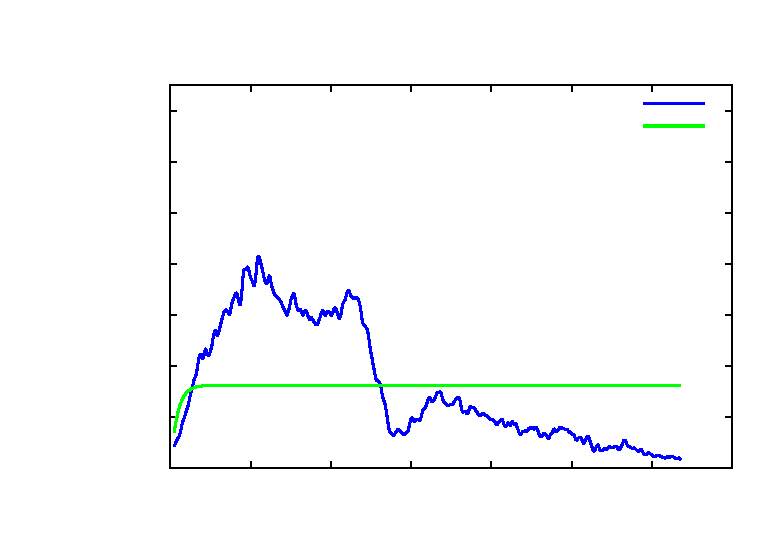
\includegraphics{img/exp1/R/invJerror_taskLhand_2}}%
    \gplfronttext
  \end{picture}%
\endgroup

    } 
    \label{fig:exp1:taskLhand2:R}
  }
  \subfigure[Both hands motion - iteration 2]{
  \resizebox{.48\textwidth}{!} {
	% GNUPLOT: LaTeX picture with Postscript
\begingroup
  \makeatletter
  \providecommand\color[2][]{%
    \GenericError{(gnuplot) \space\space\space\@spaces}{%
      Package color not loaded in conjunction with
      terminal option `colourtext'%
    }{See the gnuplot documentation for explanation.%
    }{Either use 'blacktext' in gnuplot or load the package
      color.sty in LaTeX.}%
    \renewcommand\color[2][]{}%
  }%
  \providecommand\includegraphics[2][]{%
    \GenericError{(gnuplot) \space\space\space\@spaces}{%
      Package graphicx or graphics not loaded%
    }{See the gnuplot documentation for explanation.%
    }{The gnuplot epslatex terminal needs graphicx.sty or graphics.sty.}%
    \renewcommand\includegraphics[2][]{}%
  }%
  \providecommand\rotatebox[2]{#2}%
  \@ifundefined{ifGPcolor}{%
    \newif\ifGPcolor
    \GPcolortrue
  }{}%
  \@ifundefined{ifGPblacktext}{%
    \newif\ifGPblacktext
    \GPblacktexttrue
  }{}%
  % define a \g@addto@macro without @ in the name:
  \let\gplgaddtomacro\g@addto@macro
  % define empty templates for all commands taking text:
  \gdef\gplbacktext{}%
  \gdef\gplfronttext{}%
  \makeatother
  \ifGPblacktext
    % no textcolor at all
    \def\colorrgb#1{}%
    \def\colorgray#1{}%
  \else
    % gray or color?
    \ifGPcolor
      \def\colorrgb#1{\color[rgb]{#1}}%
      \def\colorgray#1{\color[gray]{#1}}%
      \expandafter\def\csname LTw\endcsname{\color{white}}%
      \expandafter\def\csname LTb\endcsname{\color{black}}%
      \expandafter\def\csname LTa\endcsname{\color{black}}%
      \expandafter\def\csname LT0\endcsname{\color[rgb]{1,0,0}}%
      \expandafter\def\csname LT1\endcsname{\color[rgb]{0,1,0}}%
      \expandafter\def\csname LT2\endcsname{\color[rgb]{0,0,1}}%
      \expandafter\def\csname LT3\endcsname{\color[rgb]{1,0,1}}%
      \expandafter\def\csname LT4\endcsname{\color[rgb]{0,1,1}}%
      \expandafter\def\csname LT5\endcsname{\color[rgb]{1,1,0}}%
      \expandafter\def\csname LT6\endcsname{\color[rgb]{0,0,0}}%
      \expandafter\def\csname LT7\endcsname{\color[rgb]{1,0.3,0}}%
      \expandafter\def\csname LT8\endcsname{\color[rgb]{0.5,0.5,0.5}}%
    \else
      % gray
      \def\colorrgb#1{\color{black}}%
      \def\colorgray#1{\color[gray]{#1}}%
      \expandafter\def\csname LTw\endcsname{\color{white}}%
      \expandafter\def\csname LTb\endcsname{\color{black}}%
      \expandafter\def\csname LTa\endcsname{\color{black}}%
      \expandafter\def\csname LT0\endcsname{\color{black}}%
      \expandafter\def\csname LT1\endcsname{\color{black}}%
      \expandafter\def\csname LT2\endcsname{\color{black}}%
      \expandafter\def\csname LT3\endcsname{\color{black}}%
      \expandafter\def\csname LT4\endcsname{\color{black}}%
      \expandafter\def\csname LT5\endcsname{\color{black}}%
      \expandafter\def\csname LT6\endcsname{\color{black}}%
      \expandafter\def\csname LT7\endcsname{\color{black}}%
      \expandafter\def\csname LT8\endcsname{\color{black}}%
    \fi
  \fi
  \setlength{\unitlength}{0.0500bp}%
  \begin{picture}(7200.00,5040.00)%
    \gplgaddtomacro\gplbacktext{%
      \csname LTb\endcsname%
      \put(1342,704){\makebox(0,0)[r]{\strut{} 0}}%
      \put(1342,1194){\makebox(0,0)[r]{\strut{} 0.01}}%
      \put(1342,1684){\makebox(0,0)[r]{\strut{} 0.02}}%
      \put(1342,2174){\makebox(0,0)[r]{\strut{} 0.03}}%
      \put(1342,2665){\makebox(0,0)[r]{\strut{} 0.04}}%
      \put(1342,3155){\makebox(0,0)[r]{\strut{} 0.05}}%
      \put(1342,3645){\makebox(0,0)[r]{\strut{} 0.06}}%
      \put(1342,4135){\makebox(0,0)[r]{\strut{} 0.07}}%
      \put(1474,484){\makebox(0,0){\strut{} 0}}%
      \put(2245,484){\makebox(0,0){\strut{} 2}}%
      \put(3016,484){\makebox(0,0){\strut{} 4}}%
      \put(3787,484){\makebox(0,0){\strut{} 6}}%
      \put(4557,484){\makebox(0,0){\strut{} 8}}%
      \put(5328,484){\makebox(0,0){\strut{} 10}}%
      \put(6099,484){\makebox(0,0){\strut{} 12}}%
      \put(6870,484){\makebox(0,0){\strut{} 14}}%
      \put(440,2542){\rotatebox{90}{\makebox(0,0){\strut{}$\Vert \dot{q}\Vert$ (rad/s)}}}%
      \put(4172,154){\makebox(0,0){\strut{}$t$ (s)}}%
      \put(4172,4710){\makebox(0,0){\strut{}Right and left hand motion - Left hand task}}%
    }%
    \gplgaddtomacro\gplfronttext{%
      \csname LTb\endcsname%
      \put(5883,4207){\makebox(0,0)[r]{\strut{}$J^+ \dot{e}_{lhand}$}}%
      \csname LTb\endcsname%
      \put(5883,3987){\makebox(0,0)[r]{\strut{}Model}}%
    }%
    \gplbacktext
    \put(0,0){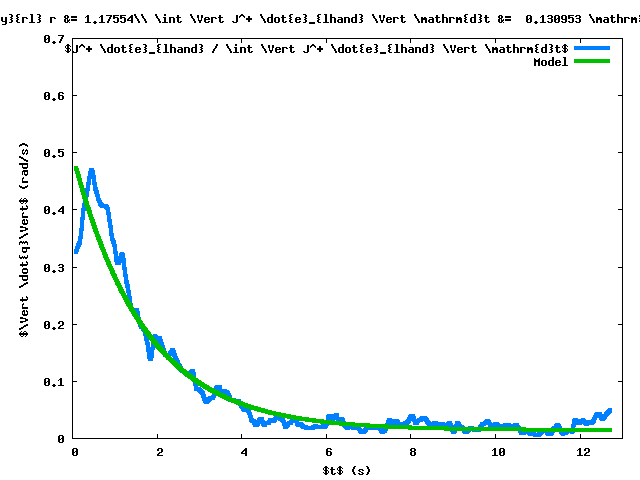
\includegraphics{img/exp1/RL/invJerror_taskLhand_2}}%
    \gplfronttext
  \end{picture}%
\endgroup

    }
    \label{fig:exp1:taskLhand2:RL}
  }
\caption{Comparison of the fitting for the left hand task for the \emph{both hands} and \emph{right hand} motion at the third iteration of the identification algorithm.
$r$ are the residues of the optimizations.}
\label{fig:exp1:taskLhand2}
\end{figure*}

satan satan satan satan satan satan satan satan satan satan satan
satan satan satan satan satan satan satan satan satan satan satan
satan satan satan satan satan satan satan satan satan satan satan
satan satan satan satan satan satan satan satan satan satan satan
satan satan satan satan satan satan satan satan satan satan satan
satan satan satan satan satan satan satan satan satan satan satan
satan satan satan satan satan satan satan satan satan satan satan
satan

\begin{figure}[t]
  \centering
  %\subfigure[Both hands motion - iteration 2]{
  \resizebox{.48\textwidth}{!} {
  \begin{tabular}{c}
	% GNUPLOT: LaTeX picture with Postscript
\begingroup
  \makeatletter
  \providecommand\color[2][]{%
    \GenericError{(gnuplot) \space\space\space\@spaces}{%
      Package color not loaded in conjunction with
      terminal option `colourtext'%
    }{See the gnuplot documentation for explanation.%
    }{Either use 'blacktext' in gnuplot or load the package
      color.sty in LaTeX.}%
    \renewcommand\color[2][]{}%
  }%
  \providecommand\includegraphics[2][]{%
    \GenericError{(gnuplot) \space\space\space\@spaces}{%
      Package graphicx or graphics not loaded%
    }{See the gnuplot documentation for explanation.%
    }{The gnuplot epslatex terminal needs graphicx.sty or graphics.sty.}%
    \renewcommand\includegraphics[2][]{}%
  }%
  \providecommand\rotatebox[2]{#2}%
  \@ifundefined{ifGPcolor}{%
    \newif\ifGPcolor
    \GPcolortrue
  }{}%
  \@ifundefined{ifGPblacktext}{%
    \newif\ifGPblacktext
    \GPblacktexttrue
  }{}%
  % define a \g@addto@macro without @ in the name:
  \let\gplgaddtomacro\g@addto@macro
  % define empty templates for all commands taking text:
  \gdef\gplbacktext{}%
  \gdef\gplfronttext{}%
  \makeatother
  \ifGPblacktext
    % no textcolor at all
    \def\colorrgb#1{}%
    \def\colorgray#1{}%
  \else
    % gray or color?
    \ifGPcolor
      \def\colorrgb#1{\color[rgb]{#1}}%
      \def\colorgray#1{\color[gray]{#1}}%
      \expandafter\def\csname LTw\endcsname{\color{white}}%
      \expandafter\def\csname LTb\endcsname{\color{black}}%
      \expandafter\def\csname LTa\endcsname{\color{black}}%
      \expandafter\def\csname LT0\endcsname{\color[rgb]{1,0,0}}%
      \expandafter\def\csname LT1\endcsname{\color[rgb]{0,1,0}}%
      \expandafter\def\csname LT2\endcsname{\color[rgb]{0,0,1}}%
      \expandafter\def\csname LT3\endcsname{\color[rgb]{1,0,1}}%
      \expandafter\def\csname LT4\endcsname{\color[rgb]{0,1,1}}%
      \expandafter\def\csname LT5\endcsname{\color[rgb]{1,1,0}}%
      \expandafter\def\csname LT6\endcsname{\color[rgb]{0,0,0}}%
      \expandafter\def\csname LT7\endcsname{\color[rgb]{1,0.3,0}}%
      \expandafter\def\csname LT8\endcsname{\color[rgb]{0.5,0.5,0.5}}%
    \else
      % gray
      \def\colorrgb#1{\color{black}}%
      \def\colorgray#1{\color[gray]{#1}}%
      \expandafter\def\csname LTw\endcsname{\color{white}}%
      \expandafter\def\csname LTb\endcsname{\color{black}}%
      \expandafter\def\csname LTa\endcsname{\color{black}}%
      \expandafter\def\csname LT0\endcsname{\color{black}}%
      \expandafter\def\csname LT1\endcsname{\color{black}}%
      \expandafter\def\csname LT2\endcsname{\color{black}}%
      \expandafter\def\csname LT3\endcsname{\color{black}}%
      \expandafter\def\csname LT4\endcsname{\color{black}}%
      \expandafter\def\csname LT5\endcsname{\color{black}}%
      \expandafter\def\csname LT6\endcsname{\color{black}}%
      \expandafter\def\csname LT7\endcsname{\color{black}}%
      \expandafter\def\csname LT8\endcsname{\color{black}}%
    \fi
  \fi
  \setlength{\unitlength}{0.0500bp}%
  \begin{picture}(7200.00,5040.00)%
    \gplgaddtomacro\gplbacktext{%
      \csname LTb\endcsname%
      \put(1210,704){\makebox(0,0)[r]{\strut{} 0}}%
      \put(1210,1229){\makebox(0,0)[r]{\strut{} 0.1}}%
      \put(1210,1754){\makebox(0,0)[r]{\strut{} 0.2}}%
      \put(1210,2279){\makebox(0,0)[r]{\strut{} 0.3}}%
      \put(1210,2805){\makebox(0,0)[r]{\strut{} 0.4}}%
      \put(1210,3330){\makebox(0,0)[r]{\strut{} 0.5}}%
      \put(1210,3855){\makebox(0,0)[r]{\strut{} 0.6}}%
      \put(1210,4380){\makebox(0,0)[r]{\strut{} 0.7}}%
      \put(1342,484){\makebox(0,0){\strut{} 0}}%
      \put(2192,484){\makebox(0,0){\strut{} 2}}%
      \put(3043,484){\makebox(0,0){\strut{} 4}}%
      \put(3893,484){\makebox(0,0){\strut{} 6}}%
      \put(4744,484){\makebox(0,0){\strut{} 8}}%
      \put(5594,484){\makebox(0,0){\strut{} 10}}%
      \put(6445,484){\makebox(0,0){\strut{} 12}}%
      \put(440,2542){\rotatebox{90}{\makebox(0,0){\strut{}$\Vert \dot{q}\Vert$ (rad/s)}}}%
      \put(4106,154){\makebox(0,0){\strut{}$t$ (s)}}%
      \put(4106,4710){\makebox(0,0){\strut{}$\begin{array}{rl} r &= 2.74842\\ \int \Vert J^+ \dot{e}_{com} \Vert \mathrm{d}t &=  0.0402254 \mathrm{rad}\\ \end{array}$}}%
    }%
    \gplgaddtomacro\gplfronttext{%
      \csname LTb\endcsname%
      \put(5883,4207){\makebox(0,0)[r]{\strut{}$J^+ \dot{e}_{com} / \int \Vert J^+ \dot{e}_{com} \Vert \mathrm{d}t$}}%
      \csname LTb\endcsname%
      \put(5883,3987){\makebox(0,0)[r]{\strut{}Model}}%
    }%
    \gplbacktext
    \put(0,0){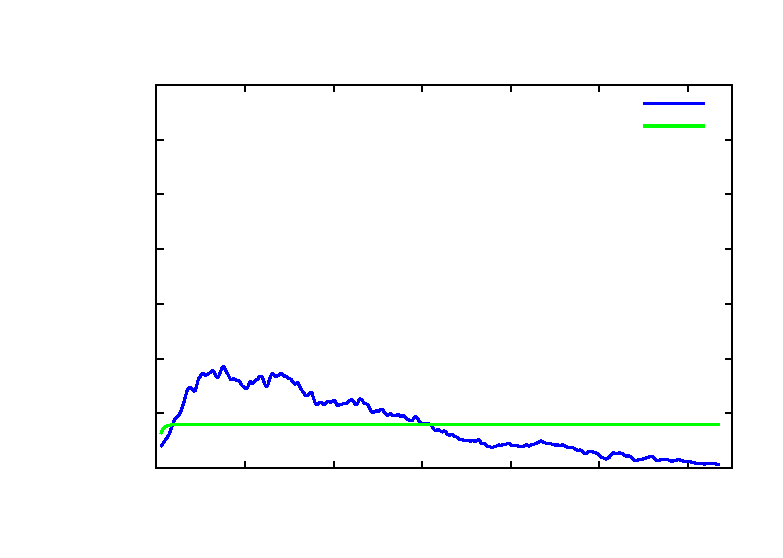
\includegraphics{img/exp1/R/invJerror_taskCom_2}}%
    \gplfronttext
  \end{picture}%
\endgroup
\\
  Right hand motion - iteration 2
  \end{tabular}
  }
  %\label{fig:exp1:taskCom2:R}
  %}
\caption{Fitting for the com task for the \emph{right hand} motion at the third iteration of the identification algorithm.
$r$ is the residue of the optimization.}
\label{fig:exp1:taskCom2}
\end{figure}

satan
satan satan satan satan satan satan satan satan satan satan satan
satan satan satan satan satan satan satan satan satan satan satan
satan satan satan satan satan satan satan satan satan satan satan
satan satan satan satan satan satan satan satan satan satan satan
satan satan satan satan satan satan satan satan satan satan satan
satan satan satan satan satan satan satan satan satan satan satan
satan satan satan satan satan satan satan satan satan satan satan
satan satan satan satan satan satan satan satan satan satan satan
satan satan satan satan satan satan satan satan satan satan satan
satan

\begin{figure}[t]
  \centering
  %\subfigure[Both hands motion - iteration 2]{
  \resizebox{.48\textwidth}{!} {
  \begin{tabular}{c}
	% GNUPLOT: LaTeX picture with Postscript
\begingroup
  \makeatletter
  \providecommand\color[2][]{%
    \GenericError{(gnuplot) \space\space\space\@spaces}{%
      Package color not loaded in conjunction with
      terminal option `colourtext'%
    }{See the gnuplot documentation for explanation.%
    }{Either use 'blacktext' in gnuplot or load the package
      color.sty in LaTeX.}%
    \renewcommand\color[2][]{}%
  }%
  \providecommand\includegraphics[2][]{%
    \GenericError{(gnuplot) \space\space\space\@spaces}{%
      Package graphicx or graphics not loaded%
    }{See the gnuplot documentation for explanation.%
    }{The gnuplot epslatex terminal needs graphicx.sty or graphics.sty.}%
    \renewcommand\includegraphics[2][]{}%
  }%
  \providecommand\rotatebox[2]{#2}%
  \@ifundefined{ifGPcolor}{%
    \newif\ifGPcolor
    \GPcolortrue
  }{}%
  \@ifundefined{ifGPblacktext}{%
    \newif\ifGPblacktext
    \GPblacktexttrue
  }{}%
  % define a \g@addto@macro without @ in the name:
  \let\gplgaddtomacro\g@addto@macro
  % define empty templates for all commands taking text:
  \gdef\gplbacktext{}%
  \gdef\gplfronttext{}%
  \makeatother
  \ifGPblacktext
    % no textcolor at all
    \def\colorrgb#1{}%
    \def\colorgray#1{}%
  \else
    % gray or color?
    \ifGPcolor
      \def\colorrgb#1{\color[rgb]{#1}}%
      \def\colorgray#1{\color[gray]{#1}}%
      \expandafter\def\csname LTw\endcsname{\color{white}}%
      \expandafter\def\csname LTb\endcsname{\color{black}}%
      \expandafter\def\csname LTa\endcsname{\color{black}}%
      \expandafter\def\csname LT0\endcsname{\color[rgb]{1,0,0}}%
      \expandafter\def\csname LT1\endcsname{\color[rgb]{0,1,0}}%
      \expandafter\def\csname LT2\endcsname{\color[rgb]{0,0,1}}%
      \expandafter\def\csname LT3\endcsname{\color[rgb]{1,0,1}}%
      \expandafter\def\csname LT4\endcsname{\color[rgb]{0,1,1}}%
      \expandafter\def\csname LT5\endcsname{\color[rgb]{1,1,0}}%
      \expandafter\def\csname LT6\endcsname{\color[rgb]{0,0,0}}%
      \expandafter\def\csname LT7\endcsname{\color[rgb]{1,0.3,0}}%
      \expandafter\def\csname LT8\endcsname{\color[rgb]{0.5,0.5,0.5}}%
    \else
      % gray
      \def\colorrgb#1{\color{black}}%
      \def\colorgray#1{\color[gray]{#1}}%
      \expandafter\def\csname LTw\endcsname{\color{white}}%
      \expandafter\def\csname LTb\endcsname{\color{black}}%
      \expandafter\def\csname LTa\endcsname{\color{black}}%
      \expandafter\def\csname LT0\endcsname{\color{black}}%
      \expandafter\def\csname LT1\endcsname{\color{black}}%
      \expandafter\def\csname LT2\endcsname{\color{black}}%
      \expandafter\def\csname LT3\endcsname{\color{black}}%
      \expandafter\def\csname LT4\endcsname{\color{black}}%
      \expandafter\def\csname LT5\endcsname{\color{black}}%
      \expandafter\def\csname LT6\endcsname{\color{black}}%
      \expandafter\def\csname LT7\endcsname{\color{black}}%
      \expandafter\def\csname LT8\endcsname{\color{black}}%
    \fi
  \fi
  \setlength{\unitlength}{0.0500bp}%
  \begin{picture}(7200.00,5040.00)%
    \gplgaddtomacro\gplbacktext{%
      \csname LTb\endcsname%
      \put(1210,704){\makebox(0,0)[r]{\strut{} 0}}%
      \put(1210,1229){\makebox(0,0)[r]{\strut{} 0.1}}%
      \put(1210,1754){\makebox(0,0)[r]{\strut{} 0.2}}%
      \put(1210,2279){\makebox(0,0)[r]{\strut{} 0.3}}%
      \put(1210,2805){\makebox(0,0)[r]{\strut{} 0.4}}%
      \put(1210,3330){\makebox(0,0)[r]{\strut{} 0.5}}%
      \put(1210,3855){\makebox(0,0)[r]{\strut{} 0.6}}%
      \put(1210,4380){\makebox(0,0)[r]{\strut{} 0.7}}%
      \put(1342,484){\makebox(0,0){\strut{} 0}}%
      \put(2192,484){\makebox(0,0){\strut{} 2}}%
      \put(3043,484){\makebox(0,0){\strut{} 4}}%
      \put(3893,484){\makebox(0,0){\strut{} 6}}%
      \put(4744,484){\makebox(0,0){\strut{} 8}}%
      \put(5594,484){\makebox(0,0){\strut{} 10}}%
      \put(6445,484){\makebox(0,0){\strut{} 12}}%
      \put(440,2542){\rotatebox{90}{\makebox(0,0){\strut{}$\Vert \dot{q}\Vert$ (rad/s)}}}%
      \put(4106,154){\makebox(0,0){\strut{}$t$ (s)}}%
      \put(4106,4710){\makebox(0,0){\strut{}$\begin{array}{rl} r &= 0.699731\\ \int \Vert J^+ \dot{e}_{twofeet} \Vert \mathrm{d}t &=  0.415981 \mathrm{rad}\\ \end{array}$}}%
    }%
    \gplgaddtomacro\gplfronttext{%
      \csname LTb\endcsname%
      \put(5883,4207){\makebox(0,0)[r]{\strut{}$J^+ \dot{e}_{twofeet} / \int \Vert J^+ \dot{e}_{twofeet} \Vert \mathrm{d}t$}}%
      \csname LTb\endcsname%
      \put(5883,3987){\makebox(0,0)[r]{\strut{}Model}}%
    }%
    \gplbacktext
    \put(0,0){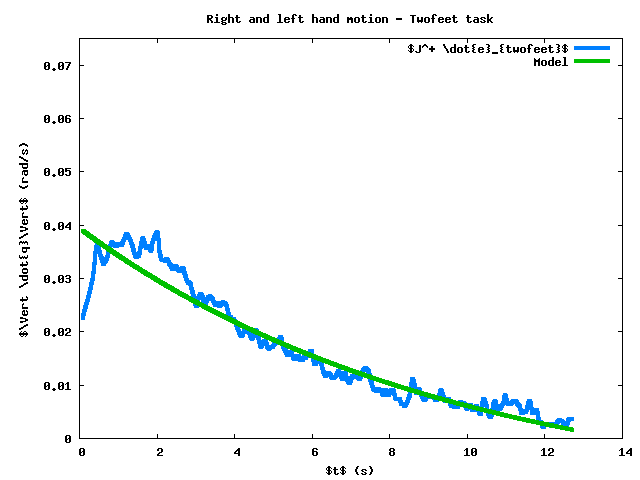
\includegraphics{img/exp1/RL/invJerror_taskTwofeet_2}}%
    \gplfronttext
  \end{picture}%
\endgroup
\\
  Both hands motion - iteration 2
  \end{tabular}
    }
  %\label{fig:exp1:taskTwofweet2:RL}
  %}
\caption{Fitting for the twofeet task for the \emph{both hands} motion at the third iteration of the identification algorithm.
$r$ is the residue of the optimization.}
\label{fig:exp1:taskTwofeet2}
\end{figure}

satan satan satan satan satan satan satan satan satan satan satan
satan satan satan satan satan satan satan satan satan satan satan
satan satan satan satan satan satan satan satan satan satan satan
satan satan satan satan satan satan satan satan satan satan satan
satan satan satan satan satan satan satan satan satan satan satan
satan satan satan satan satan satan satan satan satan satan satan
satan satan satan satan satan satan satan satan satan satan satan
satan satan satan satan satan satan satan satan satan satan satan
satan satan satan satan satan satan satan satan satan satan satan
satan satan satan satan satan satan satan satan satan satan satan
satan

%%%%%%%%%%%%%%%%%%%%%%%%%%%%%%%%%%
\begin{figure*}[t]
  %\subfigure[Both hands motion - iteration 3]{
  \resizebox{.48\textwidth}{!} {
  \begin{tabular}{c}
	% GNUPLOT: LaTeX picture with Postscript
\begingroup
  \makeatletter
  \providecommand\color[2][]{%
    \GenericError{(gnuplot) \space\space\space\@spaces}{%
      Package color not loaded in conjunction with
      terminal option `colourtext'%
    }{See the gnuplot documentation for explanation.%
    }{Either use 'blacktext' in gnuplot or load the package
      color.sty in LaTeX.}%
    \renewcommand\color[2][]{}%
  }%
  \providecommand\includegraphics[2][]{%
    \GenericError{(gnuplot) \space\space\space\@spaces}{%
      Package graphicx or graphics not loaded%
    }{See the gnuplot documentation for explanation.%
    }{The gnuplot epslatex terminal needs graphicx.sty or graphics.sty.}%
    \renewcommand\includegraphics[2][]{}%
  }%
  \providecommand\rotatebox[2]{#2}%
  \@ifundefined{ifGPcolor}{%
    \newif\ifGPcolor
    \GPcolortrue
  }{}%
  \@ifundefined{ifGPblacktext}{%
    \newif\ifGPblacktext
    \GPblacktexttrue
  }{}%
  % define a \g@addto@macro without @ in the name:
  \let\gplgaddtomacro\g@addto@macro
  % define empty templates for all commands taking text:
  \gdef\gplbacktext{}%
  \gdef\gplfronttext{}%
  \makeatother
  \ifGPblacktext
    % no textcolor at all
    \def\colorrgb#1{}%
    \def\colorgray#1{}%
  \else
    % gray or color?
    \ifGPcolor
      \def\colorrgb#1{\color[rgb]{#1}}%
      \def\colorgray#1{\color[gray]{#1}}%
      \expandafter\def\csname LTw\endcsname{\color{white}}%
      \expandafter\def\csname LTb\endcsname{\color{black}}%
      \expandafter\def\csname LTa\endcsname{\color{black}}%
      \expandafter\def\csname LT0\endcsname{\color[rgb]{1,0,0}}%
      \expandafter\def\csname LT1\endcsname{\color[rgb]{0,1,0}}%
      \expandafter\def\csname LT2\endcsname{\color[rgb]{0,0,1}}%
      \expandafter\def\csname LT3\endcsname{\color[rgb]{1,0,1}}%
      \expandafter\def\csname LT4\endcsname{\color[rgb]{0,1,1}}%
      \expandafter\def\csname LT5\endcsname{\color[rgb]{1,1,0}}%
      \expandafter\def\csname LT6\endcsname{\color[rgb]{0,0,0}}%
      \expandafter\def\csname LT7\endcsname{\color[rgb]{1,0.3,0}}%
      \expandafter\def\csname LT8\endcsname{\color[rgb]{0.5,0.5,0.5}}%
    \else
      % gray
      \def\colorrgb#1{\color{black}}%
      \def\colorgray#1{\color[gray]{#1}}%
      \expandafter\def\csname LTw\endcsname{\color{white}}%
      \expandafter\def\csname LTb\endcsname{\color{black}}%
      \expandafter\def\csname LTa\endcsname{\color{black}}%
      \expandafter\def\csname LT0\endcsname{\color{black}}%
      \expandafter\def\csname LT1\endcsname{\color{black}}%
      \expandafter\def\csname LT2\endcsname{\color{black}}%
      \expandafter\def\csname LT3\endcsname{\color{black}}%
      \expandafter\def\csname LT4\endcsname{\color{black}}%
      \expandafter\def\csname LT5\endcsname{\color{black}}%
      \expandafter\def\csname LT6\endcsname{\color{black}}%
      \expandafter\def\csname LT7\endcsname{\color{black}}%
      \expandafter\def\csname LT8\endcsname{\color{black}}%
    \fi
  \fi
  \setlength{\unitlength}{0.0500bp}%
  \begin{picture}(7200.00,5040.00)%
    \gplgaddtomacro\gplbacktext{%
      \csname LTb\endcsname%
      \put(1210,704){\makebox(0,0)[r]{\strut{} 0}}%
      \put(1210,1229){\makebox(0,0)[r]{\strut{} 0.1}}%
      \put(1210,1754){\makebox(0,0)[r]{\strut{} 0.2}}%
      \put(1210,2279){\makebox(0,0)[r]{\strut{} 0.3}}%
      \put(1210,2805){\makebox(0,0)[r]{\strut{} 0.4}}%
      \put(1210,3330){\makebox(0,0)[r]{\strut{} 0.5}}%
      \put(1210,3855){\makebox(0,0)[r]{\strut{} 0.6}}%
      \put(1210,4380){\makebox(0,0)[r]{\strut{} 0.7}}%
      \put(1342,484){\makebox(0,0){\strut{} 0}}%
      \put(2192,484){\makebox(0,0){\strut{} 2}}%
      \put(3043,484){\makebox(0,0){\strut{} 4}}%
      \put(3893,484){\makebox(0,0){\strut{} 6}}%
      \put(4744,484){\makebox(0,0){\strut{} 8}}%
      \put(5594,484){\makebox(0,0){\strut{} 10}}%
      \put(6445,484){\makebox(0,0){\strut{} 12}}%
      \put(440,2542){\rotatebox{90}{\makebox(0,0){\strut{}$\Vert \dot{q}\Vert$ (rad/s)}}}%
      \put(4106,154){\makebox(0,0){\strut{}$t$ (s)}}%
      \put(4106,4710){\makebox(0,0){\strut{}$\begin{array}{rl} r &= 2.42713\\ \int \Vert J^+ \dot{e}_{head} \Vert \mathrm{d}t &=  0.0198545 \mathrm{rad}\\ \end{array}$}}%
    }%
    \gplgaddtomacro\gplfronttext{%
      \csname LTb\endcsname%
      \put(5883,4207){\makebox(0,0)[r]{\strut{}$J^+ \dot{e}_{head} / \int \Vert J^+ \dot{e}_{head} \Vert \mathrm{d}t$}}%
      \csname LTb\endcsname%
      \put(5883,3987){\makebox(0,0)[r]{\strut{}Model}}%
    }%
    \gplbacktext
    \put(0,0){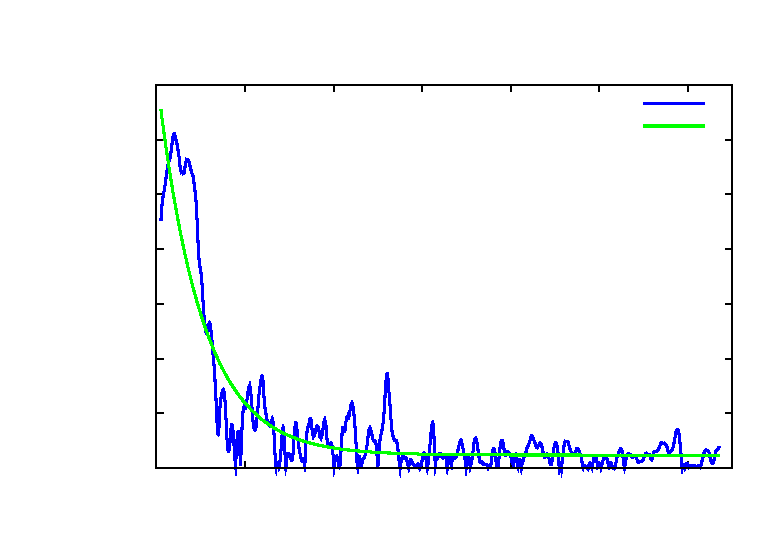
\includegraphics{img/exp1/RL/invJerror_taskHead_3}}%
    \gplfronttext
  \end{picture}%
\endgroup
\\
  Both hands motion - iteration 3
  \end{tabular}
    }
    %\label{fig:exp1:taskHead3:RL}
  %}
\caption{Comparison of the fitting for the head task for the \emph{both hands} motion at the fourth iteration of the identification algorithm.
$r$ is the residue of the optimization.}
\label{fig:exp1:taskHead3}
\end{figure*}

satan
satan satan satan satan satan satan satan satan satan satan satan
satan satan satan satan satan satan satan satan satan satan satan
satan satan satan satan satan satan satan satan satan satan satan
satan satan satan satan satan satan satan satan satan satan satan
satan satan satan satan satan satan satan satan satan satan satan
satan satan satan satan satan satan satan satan satan satan satan
satan satan satan satan satan satan satan satan satan satan satan
satan satan satan satan satan satan satan satan satan satan satan
satan satan satan satan satan satan satan satan satan satan satan
satan satan satan satan satan satan satan satan satan satan satan

\begin{figure}[t]
  \centering
  \subfigure[Both hands motion - iteration 3]{
  \resizebox{.48\textwidth}{!} {
        % GNUPLOT: LaTeX picture with Postscript
\begingroup
  \makeatletter
  \providecommand\color[2][]{%
    \GenericError{(gnuplot) \space\space\space\@spaces}{%
      Package color not loaded in conjunction with
      terminal option `colourtext'%
    }{See the gnuplot documentation for explanation.%
    }{Either use 'blacktext' in gnuplot or load the package
      color.sty in LaTeX.}%
    \renewcommand\color[2][]{}%
  }%
  \providecommand\includegraphics[2][]{%
    \GenericError{(gnuplot) \space\space\space\@spaces}{%
      Package graphicx or graphics not loaded%
    }{See the gnuplot documentation for explanation.%
    }{The gnuplot epslatex terminal needs graphicx.sty or graphics.sty.}%
    \renewcommand\includegraphics[2][]{}%
  }%
  \providecommand\rotatebox[2]{#2}%
  \@ifundefined{ifGPcolor}{%
    \newif\ifGPcolor
    \GPcolortrue
  }{}%
  \@ifundefined{ifGPblacktext}{%
    \newif\ifGPblacktext
    \GPblacktexttrue
  }{}%
  % define a \g@addto@macro without @ in the name:
  \let\gplgaddtomacro\g@addto@macro
  % define empty templates for all commands taking text:
  \gdef\gplbacktext{}%
  \gdef\gplfronttext{}%
  \makeatother
  \ifGPblacktext
    % no textcolor at all
    \def\colorrgb#1{}%
    \def\colorgray#1{}%
  \else
    % gray or color?
    \ifGPcolor
      \def\colorrgb#1{\color[rgb]{#1}}%
      \def\colorgray#1{\color[gray]{#1}}%
      \expandafter\def\csname LTw\endcsname{\color{white}}%
      \expandafter\def\csname LTb\endcsname{\color{black}}%
      \expandafter\def\csname LTa\endcsname{\color{black}}%
      \expandafter\def\csname LT0\endcsname{\color[rgb]{1,0,0}}%
      \expandafter\def\csname LT1\endcsname{\color[rgb]{0,1,0}}%
      \expandafter\def\csname LT2\endcsname{\color[rgb]{0,0,1}}%
      \expandafter\def\csname LT3\endcsname{\color[rgb]{1,0,1}}%
      \expandafter\def\csname LT4\endcsname{\color[rgb]{0,1,1}}%
      \expandafter\def\csname LT5\endcsname{\color[rgb]{1,1,0}}%
      \expandafter\def\csname LT6\endcsname{\color[rgb]{0,0,0}}%
      \expandafter\def\csname LT7\endcsname{\color[rgb]{1,0.3,0}}%
      \expandafter\def\csname LT8\endcsname{\color[rgb]{0.5,0.5,0.5}}%
    \else
      % gray
      \def\colorrgb#1{\color{black}}%
      \def\colorgray#1{\color[gray]{#1}}%
      \expandafter\def\csname LTw\endcsname{\color{white}}%
      \expandafter\def\csname LTb\endcsname{\color{black}}%
      \expandafter\def\csname LTa\endcsname{\color{black}}%
      \expandafter\def\csname LT0\endcsname{\color{black}}%
      \expandafter\def\csname LT1\endcsname{\color{black}}%
      \expandafter\def\csname LT2\endcsname{\color{black}}%
      \expandafter\def\csname LT3\endcsname{\color{black}}%
      \expandafter\def\csname LT4\endcsname{\color{black}}%
      \expandafter\def\csname LT5\endcsname{\color{black}}%
      \expandafter\def\csname LT6\endcsname{\color{black}}%
      \expandafter\def\csname LT7\endcsname{\color{black}}%
      \expandafter\def\csname LT8\endcsname{\color{black}}%
    \fi
  \fi
  \setlength{\unitlength}{0.0500bp}%
  \begin{picture}(7200.00,5040.00)%
    \gplgaddtomacro\gplbacktext{%
      \csname LTb\endcsname%
      \put(1342,704){\makebox(0,0)[r]{\strut{} 0}}%
      \put(1342,1194){\makebox(0,0)[r]{\strut{} 0.01}}%
      \put(1342,1684){\makebox(0,0)[r]{\strut{} 0.02}}%
      \put(1342,2174){\makebox(0,0)[r]{\strut{} 0.03}}%
      \put(1342,2665){\makebox(0,0)[r]{\strut{} 0.04}}%
      \put(1342,3155){\makebox(0,0)[r]{\strut{} 0.05}}%
      \put(1342,3645){\makebox(0,0)[r]{\strut{} 0.06}}%
      \put(1342,4135){\makebox(0,0)[r]{\strut{} 0.07}}%
      \put(1474,484){\makebox(0,0){\strut{} 0}}%
      \put(2245,484){\makebox(0,0){\strut{} 2}}%
      \put(3016,484){\makebox(0,0){\strut{} 4}}%
      \put(3787,484){\makebox(0,0){\strut{} 6}}%
      \put(4557,484){\makebox(0,0){\strut{} 8}}%
      \put(5328,484){\makebox(0,0){\strut{} 10}}%
      \put(6099,484){\makebox(0,0){\strut{} 12}}%
      \put(6870,484){\makebox(0,0){\strut{} 14}}%
      \put(440,2542){\rotatebox{90}{\makebox(0,0){\strut{}$\Vert \dot{q}\Vert$ (rad/s)}}}%
      \put(4172,154){\makebox(0,0){\strut{}$t$ (s)}}%
      \put(4172,4710){\makebox(0,0){\strut{}Right and left hand motion - Left hand task}}%
    }%
    \gplgaddtomacro\gplfronttext{%
      \csname LTb\endcsname%
      \put(5883,4207){\makebox(0,0)[r]{\strut{}$J^+ \dot{e}_{lhand}$}}%
      \csname LTb\endcsname%
      \put(5883,3987){\makebox(0,0)[r]{\strut{}Model}}%
    }%
    \gplbacktext
    \put(0,0){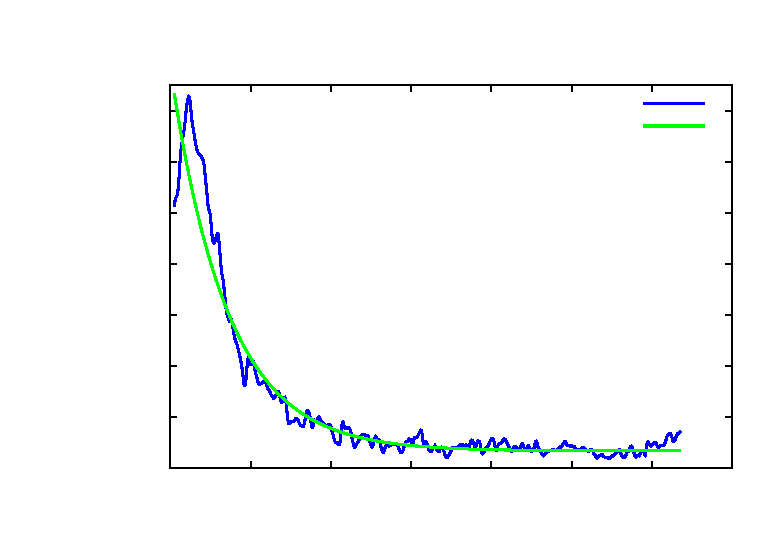
\includegraphics{img/exp1/RL/invJerror_taskLhand_3}}%
    \gplfronttext
  \end{picture}%
\endgroup

    }
    %\label{fig:exp1:taskLhand3:RL}
  }
\caption{Comparison of the fitting for the left hand task for the \emph{both hands} motion at the fourth iteration of the identification algorithm.
$r$ are the residues of the optimizations.}
\label{fig:exp1:taskLhand3}
\end{figure}

satan
satan satan satan satan satan satan satan satan satan satan satan
satan satan satan satan satan satan satan satan satan satan satan
satan satan satan satan satan satan satan satan satan satan satan
satan satan satan satan satan satan satan satan satan satan satan
satan satan satan satan satan satan satan satan satan satan satan
satan satan satan satan satan satan satan satan satan satan satan
satan satan satan satan satan satan satan satan satan satan satan
satan satan satan satan satan satan satan satan satan satan satan
satan satan satan satan satan satan satan satan satan satan satan
satan satan satan satan satan satan satan satan satan satan satan
satan satan satan satan satan satan satan satan satan satan satan
satan satan satan satan satan satan satan satan satan satan satan
satan satan satan satan satan satan satan satan satan satan satan
satan satan satan satan satan satan satan satan satan satan satan

\begin{figure*}[t]
\centering
\begin{tabular}{|c|c|}
  \hline
  Right hand motion & Both hands motion\\
  \hline
    \resizebox{.43\textwidth}{!}{
      % GNUPLOT: LaTeX picture with Postscript
\begingroup
  \makeatletter
  \providecommand\color[2][]{%
    \GenericError{(gnuplot) \space\space\space\@spaces}{%
      Package color not loaded in conjunction with
      terminal option `colourtext'%
    }{See the gnuplot documentation for explanation.%
    }{Either use 'blacktext' in gnuplot or load the package
      color.sty in LaTeX.}%
    \renewcommand\color[2][]{}%
  }%
  \providecommand\includegraphics[2][]{%
    \GenericError{(gnuplot) \space\space\space\@spaces}{%
      Package graphicx or graphics not loaded%
    }{See the gnuplot documentation for explanation.%
    }{The gnuplot epslatex terminal needs graphicx.sty or graphics.sty.}%
    \renewcommand\includegraphics[2][]{}%
  }%
  \providecommand\rotatebox[2]{#2}%
  \@ifundefined{ifGPcolor}{%
    \newif\ifGPcolor
    \GPcolortrue
  }{}%
  \@ifundefined{ifGPblacktext}{%
    \newif\ifGPblacktext
    \GPblacktexttrue
  }{}%
  % define a \g@addto@macro without @ in the name:
  \let\gplgaddtomacro\g@addto@macro
  % define empty templates for all commands taking text:
  \gdef\gplbacktext{}%
  \gdef\gplfronttext{}%
  \makeatother
  \ifGPblacktext
    % no textcolor at all
    \def\colorrgb#1{}%
    \def\colorgray#1{}%
  \else
    % gray or color?
    \ifGPcolor
      \def\colorrgb#1{\color[rgb]{#1}}%
      \def\colorgray#1{\color[gray]{#1}}%
      \expandafter\def\csname LTw\endcsname{\color{white}}%
      \expandafter\def\csname LTb\endcsname{\color{black}}%
      \expandafter\def\csname LTa\endcsname{\color{black}}%
      \expandafter\def\csname LT0\endcsname{\color[rgb]{1,0,0}}%
      \expandafter\def\csname LT1\endcsname{\color[rgb]{0,1,0}}%
      \expandafter\def\csname LT2\endcsname{\color[rgb]{0,0,1}}%
      \expandafter\def\csname LT3\endcsname{\color[rgb]{1,0,1}}%
      \expandafter\def\csname LT4\endcsname{\color[rgb]{0,1,1}}%
      \expandafter\def\csname LT5\endcsname{\color[rgb]{1,1,0}}%
      \expandafter\def\csname LT6\endcsname{\color[rgb]{0,0,0}}%
      \expandafter\def\csname LT7\endcsname{\color[rgb]{1,0.3,0}}%
      \expandafter\def\csname LT8\endcsname{\color[rgb]{0.5,0.5,0.5}}%
    \else
      % gray
      \def\colorrgb#1{\color{black}}%
      \def\colorgray#1{\color[gray]{#1}}%
      \expandafter\def\csname LTw\endcsname{\color{white}}%
      \expandafter\def\csname LTb\endcsname{\color{black}}%
      \expandafter\def\csname LTa\endcsname{\color{black}}%
      \expandafter\def\csname LT0\endcsname{\color{black}}%
      \expandafter\def\csname LT1\endcsname{\color{black}}%
      \expandafter\def\csname LT2\endcsname{\color{black}}%
      \expandafter\def\csname LT3\endcsname{\color{black}}%
      \expandafter\def\csname LT4\endcsname{\color{black}}%
      \expandafter\def\csname LT5\endcsname{\color{black}}%
      \expandafter\def\csname LT6\endcsname{\color{black}}%
      \expandafter\def\csname LT7\endcsname{\color{black}}%
      \expandafter\def\csname LT8\endcsname{\color{black}}%
    \fi
  \fi
  \setlength{\unitlength}{0.0500bp}%
  \begin{picture}(7200.00,5040.00)%
    \gplgaddtomacro\gplbacktext{%
      \csname LTb\endcsname%
      \put(1342,704){\makebox(0,0)[r]{\strut{} 0}}%
      \put(1342,1194){\makebox(0,0)[r]{\strut{} 0.01}}%
      \put(1342,1684){\makebox(0,0)[r]{\strut{} 0.02}}%
      \put(1342,2174){\makebox(0,0)[r]{\strut{} 0.03}}%
      \put(1342,2665){\makebox(0,0)[r]{\strut{} 0.04}}%
      \put(1342,3155){\makebox(0,0)[r]{\strut{} 0.05}}%
      \put(1342,3645){\makebox(0,0)[r]{\strut{} 0.06}}%
      \put(1342,4135){\makebox(0,0)[r]{\strut{} 0.07}}%
      \put(1474,484){\makebox(0,0){\strut{} 0}}%
      \put(2245,484){\makebox(0,0){\strut{} 2}}%
      \put(3016,484){\makebox(0,0){\strut{} 4}}%
      \put(3787,484){\makebox(0,0){\strut{} 6}}%
      \put(4557,484){\makebox(0,0){\strut{} 8}}%
      \put(5328,484){\makebox(0,0){\strut{} 10}}%
      \put(6099,484){\makebox(0,0){\strut{} 12}}%
      \put(6870,484){\makebox(0,0){\strut{} 14}}%
      \put(440,2542){\rotatebox{90}{\makebox(0,0){\strut{}$\Vert \dot{q}\Vert$ (rad/s)}}}%
      \put(4172,154){\makebox(0,0){\strut{}$t$ (s)}}%
      \put(4172,4710){\makebox(0,0){\strut{}Right hand motion - Right Hand task}}%
    }%
    \gplgaddtomacro\gplfronttext{%
      \csname LTb\endcsname%
      \put(5883,4207){\makebox(0,0)[r]{\strut{}$J^+ \dot{e}_{rhand}$}}%
      \csname LTb\endcsname%
      \put(5883,3987){\makebox(0,0)[r]{\strut{}Model}}%
    }%
    \gplbacktext
    \put(0,0){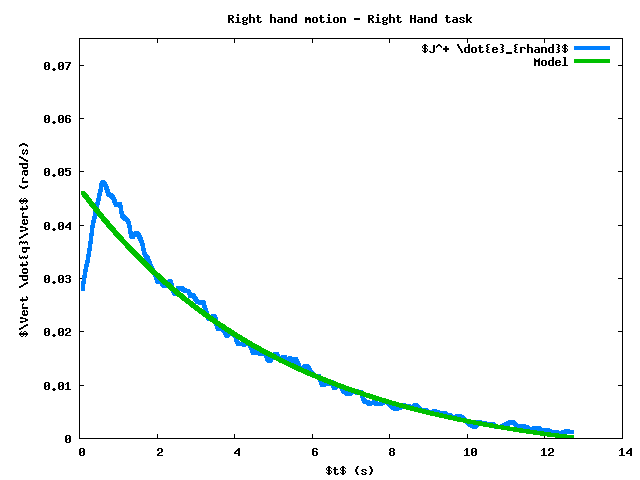
\includegraphics{img/exp1/R/invJerror_taskRhand_0}}%
    \gplfronttext
  \end{picture}%
\endgroup

    }
  &
    \resizebox{.43\textwidth}{!}{
      % GNUPLOT: LaTeX picture with Postscript
\begingroup
  \makeatletter
  \providecommand\color[2][]{%
    \GenericError{(gnuplot) \space\space\space\@spaces}{%
      Package color not loaded in conjunction with
      terminal option `colourtext'%
    }{See the gnuplot documentation for explanation.%
    }{Either use 'blacktext' in gnuplot or load the package
      color.sty in LaTeX.}%
    \renewcommand\color[2][]{}%
  }%
  \providecommand\includegraphics[2][]{%
    \GenericError{(gnuplot) \space\space\space\@spaces}{%
      Package graphicx or graphics not loaded%
    }{See the gnuplot documentation for explanation.%
    }{The gnuplot epslatex terminal needs graphicx.sty or graphics.sty.}%
    \renewcommand\includegraphics[2][]{}%
  }%
  \providecommand\rotatebox[2]{#2}%
  \@ifundefined{ifGPcolor}{%
    \newif\ifGPcolor
    \GPcolortrue
  }{}%
  \@ifundefined{ifGPblacktext}{%
    \newif\ifGPblacktext
    \GPblacktexttrue
  }{}%
  % define a \g@addto@macro without @ in the name:
  \let\gplgaddtomacro\g@addto@macro
  % define empty templates for all commands taking text:
  \gdef\gplbacktext{}%
  \gdef\gplfronttext{}%
  \makeatother
  \ifGPblacktext
    % no textcolor at all
    \def\colorrgb#1{}%
    \def\colorgray#1{}%
  \else
    % gray or color?
    \ifGPcolor
      \def\colorrgb#1{\color[rgb]{#1}}%
      \def\colorgray#1{\color[gray]{#1}}%
      \expandafter\def\csname LTw\endcsname{\color{white}}%
      \expandafter\def\csname LTb\endcsname{\color{black}}%
      \expandafter\def\csname LTa\endcsname{\color{black}}%
      \expandafter\def\csname LT0\endcsname{\color[rgb]{1,0,0}}%
      \expandafter\def\csname LT1\endcsname{\color[rgb]{0,1,0}}%
      \expandafter\def\csname LT2\endcsname{\color[rgb]{0,0,1}}%
      \expandafter\def\csname LT3\endcsname{\color[rgb]{1,0,1}}%
      \expandafter\def\csname LT4\endcsname{\color[rgb]{0,1,1}}%
      \expandafter\def\csname LT5\endcsname{\color[rgb]{1,1,0}}%
      \expandafter\def\csname LT6\endcsname{\color[rgb]{0,0,0}}%
      \expandafter\def\csname LT7\endcsname{\color[rgb]{1,0.3,0}}%
      \expandafter\def\csname LT8\endcsname{\color[rgb]{0.5,0.5,0.5}}%
    \else
      % gray
      \def\colorrgb#1{\color{black}}%
      \def\colorgray#1{\color[gray]{#1}}%
      \expandafter\def\csname LTw\endcsname{\color{white}}%
      \expandafter\def\csname LTb\endcsname{\color{black}}%
      \expandafter\def\csname LTa\endcsname{\color{black}}%
      \expandafter\def\csname LT0\endcsname{\color{black}}%
      \expandafter\def\csname LT1\endcsname{\color{black}}%
      \expandafter\def\csname LT2\endcsname{\color{black}}%
      \expandafter\def\csname LT3\endcsname{\color{black}}%
      \expandafter\def\csname LT4\endcsname{\color{black}}%
      \expandafter\def\csname LT5\endcsname{\color{black}}%
      \expandafter\def\csname LT6\endcsname{\color{black}}%
      \expandafter\def\csname LT7\endcsname{\color{black}}%
      \expandafter\def\csname LT8\endcsname{\color{black}}%
    \fi
  \fi
  \setlength{\unitlength}{0.0500bp}%
  \begin{picture}(7200.00,5040.00)%
    \gplgaddtomacro\gplbacktext{%
      \csname LTb\endcsname%
      \put(1210,704){\makebox(0,0)[r]{\strut{} 0}}%
      \put(1210,1229){\makebox(0,0)[r]{\strut{} 0.1}}%
      \put(1210,1754){\makebox(0,0)[r]{\strut{} 0.2}}%
      \put(1210,2279){\makebox(0,0)[r]{\strut{} 0.3}}%
      \put(1210,2805){\makebox(0,0)[r]{\strut{} 0.4}}%
      \put(1210,3330){\makebox(0,0)[r]{\strut{} 0.5}}%
      \put(1210,3855){\makebox(0,0)[r]{\strut{} 0.6}}%
      \put(1210,4380){\makebox(0,0)[r]{\strut{} 0.7}}%
      \put(1342,484){\makebox(0,0){\strut{} 0}}%
      \put(2192,484){\makebox(0,0){\strut{} 2}}%
      \put(3043,484){\makebox(0,0){\strut{} 4}}%
      \put(3893,484){\makebox(0,0){\strut{} 6}}%
      \put(4744,484){\makebox(0,0){\strut{} 8}}%
      \put(5594,484){\makebox(0,0){\strut{} 10}}%
      \put(6445,484){\makebox(0,0){\strut{} 12}}%
      \put(440,2542){\rotatebox{90}{\makebox(0,0){\strut{}$\Vert \dot{q}\Vert$ (rad/s)}}}%
      \put(4106,154){\makebox(0,0){\strut{}$t$ (s)}}%
      \put(4106,4710){\makebox(0,0){\strut{}$\begin{array}{rl} r &= 0.47739\\ \int \Vert J^+ \dot{e}_{rhand} \Vert \mathrm{d}t &=  0.356896 \mathrm{rad}\\ \end{array}$}}%
    }%
    \gplgaddtomacro\gplfronttext{%
      \csname LTb\endcsname%
      \put(5883,4207){\makebox(0,0)[r]{\strut{}$J^+ \dot{e}_{rhand} / \int \Vert J^+ \dot{e}_{rhand} \Vert \mathrm{d}t$}}%
      \csname LTb\endcsname%
      \put(5883,3987){\makebox(0,0)[r]{\strut{}Model}}%
    }%
    \gplbacktext
    \put(0,0){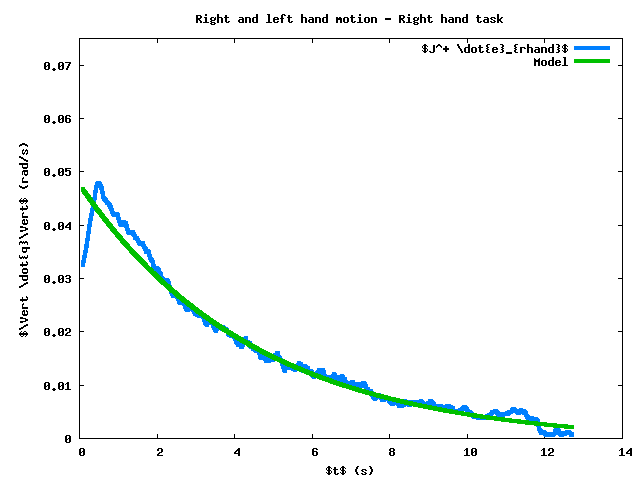
\includegraphics{img/exp1/RL/invJerror_taskRhand_0}}%
    \gplfronttext
  \end{picture}%
\endgroup

    }\\
  \hline
\end{tabular}
\caption{Right hand task fiting for \emph{right hand} and \emph{both hands} motion.}
\end{figure*}

satan
satan satan satan satan satan satan satan satan satan satan satan
satan satan satan satan satan satan satan satan satan satan satan
satan satan satan satan satan satan satan satan satan satan satan
satan satan satan satan satan satan satan satan satan satan satan
satan satan satan satan satan satan satan satan satan satan satan
satan satan satan satan satan satan satan satan satan satan satan
satan satan satan satan satan satan satan satan satan satan satan
satan satan satan satan satan satan satan satan satan satan satan
satan satan satan satan satan satan satan satan satan satan satan
satan satan satan satan satan satan satan satan satan satan satan
satan satan satan satan satan satan satan satan satan satan satan
satan satan satan satan satan satan satan satan satan satan satan
satan satan satan satan satan satan satan satan satan satan satan
satan satan satan satan satan satan satan satan satan satan satan

\begin{figure*}[t]
\centering
\begin{tabular}{|c|c|}
  \hline
  Right hand motion & Both hands motion\\
  \hline
  \subfigure{
    \resizebox{.43\textwidth}{!}{
      % GNUPLOT: LaTeX picture with Postscript
\begingroup
  \makeatletter
  \providecommand\color[2][]{%
    \GenericError{(gnuplot) \space\space\space\@spaces}{%
      Package color not loaded in conjunction with
      terminal option `colourtext'%
    }{See the gnuplot documentation for explanation.%
    }{Either use 'blacktext' in gnuplot or load the package
      color.sty in LaTeX.}%
    \renewcommand\color[2][]{}%
  }%
  \providecommand\includegraphics[2][]{%
    \GenericError{(gnuplot) \space\space\space\@spaces}{%
      Package graphicx or graphics not loaded%
    }{See the gnuplot documentation for explanation.%
    }{The gnuplot epslatex terminal needs graphicx.sty or graphics.sty.}%
    \renewcommand\includegraphics[2][]{}%
  }%
  \providecommand\rotatebox[2]{#2}%
  \@ifundefined{ifGPcolor}{%
    \newif\ifGPcolor
    \GPcolortrue
  }{}%
  \@ifundefined{ifGPblacktext}{%
    \newif\ifGPblacktext
    \GPblacktexttrue
  }{}%
  % define a \g@addto@macro without @ in the name:
  \let\gplgaddtomacro\g@addto@macro
  % define empty templates for all commands taking text:
  \gdef\gplbacktext{}%
  \gdef\gplfronttext{}%
  \makeatother
  \ifGPblacktext
    % no textcolor at all
    \def\colorrgb#1{}%
    \def\colorgray#1{}%
  \else
    % gray or color?
    \ifGPcolor
      \def\colorrgb#1{\color[rgb]{#1}}%
      \def\colorgray#1{\color[gray]{#1}}%
      \expandafter\def\csname LTw\endcsname{\color{white}}%
      \expandafter\def\csname LTb\endcsname{\color{black}}%
      \expandafter\def\csname LTa\endcsname{\color{black}}%
      \expandafter\def\csname LT0\endcsname{\color[rgb]{1,0,0}}%
      \expandafter\def\csname LT1\endcsname{\color[rgb]{0,1,0}}%
      \expandafter\def\csname LT2\endcsname{\color[rgb]{0,0,1}}%
      \expandafter\def\csname LT3\endcsname{\color[rgb]{1,0,1}}%
      \expandafter\def\csname LT4\endcsname{\color[rgb]{0,1,1}}%
      \expandafter\def\csname LT5\endcsname{\color[rgb]{1,1,0}}%
      \expandafter\def\csname LT6\endcsname{\color[rgb]{0,0,0}}%
      \expandafter\def\csname LT7\endcsname{\color[rgb]{1,0.3,0}}%
      \expandafter\def\csname LT8\endcsname{\color[rgb]{0.5,0.5,0.5}}%
    \else
      % gray
      \def\colorrgb#1{\color{black}}%
      \def\colorgray#1{\color[gray]{#1}}%
      \expandafter\def\csname LTw\endcsname{\color{white}}%
      \expandafter\def\csname LTb\endcsname{\color{black}}%
      \expandafter\def\csname LTa\endcsname{\color{black}}%
      \expandafter\def\csname LT0\endcsname{\color{black}}%
      \expandafter\def\csname LT1\endcsname{\color{black}}%
      \expandafter\def\csname LT2\endcsname{\color{black}}%
      \expandafter\def\csname LT3\endcsname{\color{black}}%
      \expandafter\def\csname LT4\endcsname{\color{black}}%
      \expandafter\def\csname LT5\endcsname{\color{black}}%
      \expandafter\def\csname LT6\endcsname{\color{black}}%
      \expandafter\def\csname LT7\endcsname{\color{black}}%
      \expandafter\def\csname LT8\endcsname{\color{black}}%
    \fi
  \fi
  \setlength{\unitlength}{0.0500bp}%
  \begin{picture}(7200.00,5040.00)%
    \gplgaddtomacro\gplbacktext{%
      \csname LTb\endcsname%
      \put(1342,704){\makebox(0,0)[r]{\strut{} 0}}%
      \put(1342,1194){\makebox(0,0)[r]{\strut{} 0.01}}%
      \put(1342,1684){\makebox(0,0)[r]{\strut{} 0.02}}%
      \put(1342,2174){\makebox(0,0)[r]{\strut{} 0.03}}%
      \put(1342,2665){\makebox(0,0)[r]{\strut{} 0.04}}%
      \put(1342,3155){\makebox(0,0)[r]{\strut{} 0.05}}%
      \put(1342,3645){\makebox(0,0)[r]{\strut{} 0.06}}%
      \put(1342,4135){\makebox(0,0)[r]{\strut{} 0.07}}%
      \put(1474,484){\makebox(0,0){\strut{} 0}}%
      \put(2245,484){\makebox(0,0){\strut{} 2}}%
      \put(3016,484){\makebox(0,0){\strut{} 4}}%
      \put(3787,484){\makebox(0,0){\strut{} 6}}%
      \put(4557,484){\makebox(0,0){\strut{} 8}}%
      \put(5328,484){\makebox(0,0){\strut{} 10}}%
      \put(6099,484){\makebox(0,0){\strut{} 12}}%
      \put(6870,484){\makebox(0,0){\strut{} 14}}%
      \put(440,2542){\rotatebox{90}{\makebox(0,0){\strut{}$\Vert \dot{q}\Vert$ (rad/s)}}}%
      \put(4172,154){\makebox(0,0){\strut{}$t$ (s)}}%
      \put(4172,4710){\makebox(0,0){\strut{}Right hand motion - Left Hand task}}%
    }%
    \gplgaddtomacro\gplfronttext{%
      \csname LTb\endcsname%
      \put(5883,4207){\makebox(0,0)[r]{\strut{}$J^+ \dot{e}_{lhand}$}}%
      \csname LTb\endcsname%
      \put(5883,3987){\makebox(0,0)[r]{\strut{}Model}}%
    }%
    \gplbacktext
    \put(0,0){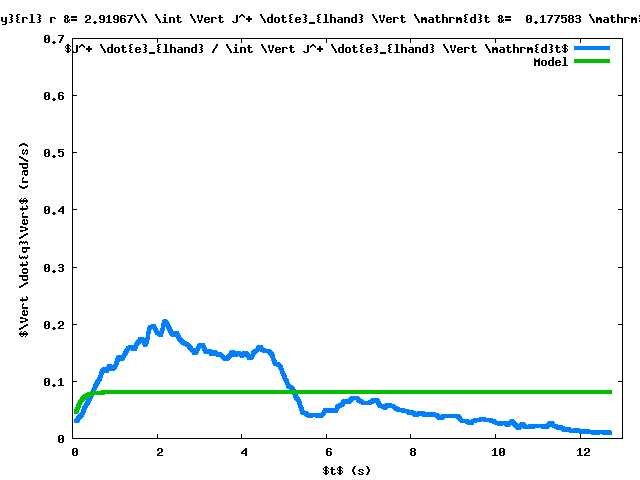
\includegraphics{img/exp1/R/invJerror_taskLhand_0}}%
    \gplfronttext
  \end{picture}%
\endgroup

    }
  }
  &
  \subfigure{
    \resizebox{.43\textwidth}{!}{
      % GNUPLOT: LaTeX picture with Postscript
\begingroup
  \makeatletter
  \providecommand\color[2][]{%
    \GenericError{(gnuplot) \space\space\space\@spaces}{%
      Package color not loaded in conjunction with
      terminal option `colourtext'%
    }{See the gnuplot documentation for explanation.%
    }{Either use 'blacktext' in gnuplot or load the package
      color.sty in LaTeX.}%
    \renewcommand\color[2][]{}%
  }%
  \providecommand\includegraphics[2][]{%
    \GenericError{(gnuplot) \space\space\space\@spaces}{%
      Package graphicx or graphics not loaded%
    }{See the gnuplot documentation for explanation.%
    }{The gnuplot epslatex terminal needs graphicx.sty or graphics.sty.}%
    \renewcommand\includegraphics[2][]{}%
  }%
  \providecommand\rotatebox[2]{#2}%
  \@ifundefined{ifGPcolor}{%
    \newif\ifGPcolor
    \GPcolortrue
  }{}%
  \@ifundefined{ifGPblacktext}{%
    \newif\ifGPblacktext
    \GPblacktexttrue
  }{}%
  % define a \g@addto@macro without @ in the name:
  \let\gplgaddtomacro\g@addto@macro
  % define empty templates for all commands taking text:
  \gdef\gplbacktext{}%
  \gdef\gplfronttext{}%
  \makeatother
  \ifGPblacktext
    % no textcolor at all
    \def\colorrgb#1{}%
    \def\colorgray#1{}%
  \else
    % gray or color?
    \ifGPcolor
      \def\colorrgb#1{\color[rgb]{#1}}%
      \def\colorgray#1{\color[gray]{#1}}%
      \expandafter\def\csname LTw\endcsname{\color{white}}%
      \expandafter\def\csname LTb\endcsname{\color{black}}%
      \expandafter\def\csname LTa\endcsname{\color{black}}%
      \expandafter\def\csname LT0\endcsname{\color[rgb]{1,0,0}}%
      \expandafter\def\csname LT1\endcsname{\color[rgb]{0,1,0}}%
      \expandafter\def\csname LT2\endcsname{\color[rgb]{0,0,1}}%
      \expandafter\def\csname LT3\endcsname{\color[rgb]{1,0,1}}%
      \expandafter\def\csname LT4\endcsname{\color[rgb]{0,1,1}}%
      \expandafter\def\csname LT5\endcsname{\color[rgb]{1,1,0}}%
      \expandafter\def\csname LT6\endcsname{\color[rgb]{0,0,0}}%
      \expandafter\def\csname LT7\endcsname{\color[rgb]{1,0.3,0}}%
      \expandafter\def\csname LT8\endcsname{\color[rgb]{0.5,0.5,0.5}}%
    \else
      % gray
      \def\colorrgb#1{\color{black}}%
      \def\colorgray#1{\color[gray]{#1}}%
      \expandafter\def\csname LTw\endcsname{\color{white}}%
      \expandafter\def\csname LTb\endcsname{\color{black}}%
      \expandafter\def\csname LTa\endcsname{\color{black}}%
      \expandafter\def\csname LT0\endcsname{\color{black}}%
      \expandafter\def\csname LT1\endcsname{\color{black}}%
      \expandafter\def\csname LT2\endcsname{\color{black}}%
      \expandafter\def\csname LT3\endcsname{\color{black}}%
      \expandafter\def\csname LT4\endcsname{\color{black}}%
      \expandafter\def\csname LT5\endcsname{\color{black}}%
      \expandafter\def\csname LT6\endcsname{\color{black}}%
      \expandafter\def\csname LT7\endcsname{\color{black}}%
      \expandafter\def\csname LT8\endcsname{\color{black}}%
    \fi
  \fi
  \setlength{\unitlength}{0.0500bp}%
  \begin{picture}(7200.00,5040.00)%
    \gplgaddtomacro\gplbacktext{%
      \csname LTb\endcsname%
      \put(1342,704){\makebox(0,0)[r]{\strut{} 0}}%
      \put(1342,1194){\makebox(0,0)[r]{\strut{} 0.01}}%
      \put(1342,1684){\makebox(0,0)[r]{\strut{} 0.02}}%
      \put(1342,2174){\makebox(0,0)[r]{\strut{} 0.03}}%
      \put(1342,2665){\makebox(0,0)[r]{\strut{} 0.04}}%
      \put(1342,3155){\makebox(0,0)[r]{\strut{} 0.05}}%
      \put(1342,3645){\makebox(0,0)[r]{\strut{} 0.06}}%
      \put(1342,4135){\makebox(0,0)[r]{\strut{} 0.07}}%
      \put(1474,484){\makebox(0,0){\strut{} 0}}%
      \put(2245,484){\makebox(0,0){\strut{} 2}}%
      \put(3016,484){\makebox(0,0){\strut{} 4}}%
      \put(3787,484){\makebox(0,0){\strut{} 6}}%
      \put(4557,484){\makebox(0,0){\strut{} 8}}%
      \put(5328,484){\makebox(0,0){\strut{} 10}}%
      \put(6099,484){\makebox(0,0){\strut{} 12}}%
      \put(6870,484){\makebox(0,0){\strut{} 14}}%
      \put(440,2542){\rotatebox{90}{\makebox(0,0){\strut{}$\Vert \dot{q}\Vert$ (rad/s)}}}%
      \put(4172,154){\makebox(0,0){\strut{}$t$ (s)}}%
      \put(4172,4710){\makebox(0,0){\strut{}Right and left hand motion - Left hand task}}%
    }%
    \gplgaddtomacro\gplfronttext{%
      \csname LTb\endcsname%
      \put(5883,4207){\makebox(0,0)[r]{\strut{}$J^+ \dot{e}_{lhand}$}}%
      \csname LTb\endcsname%
      \put(5883,3987){\makebox(0,0)[r]{\strut{}Model}}%
    }%
    \gplbacktext
    \put(0,0){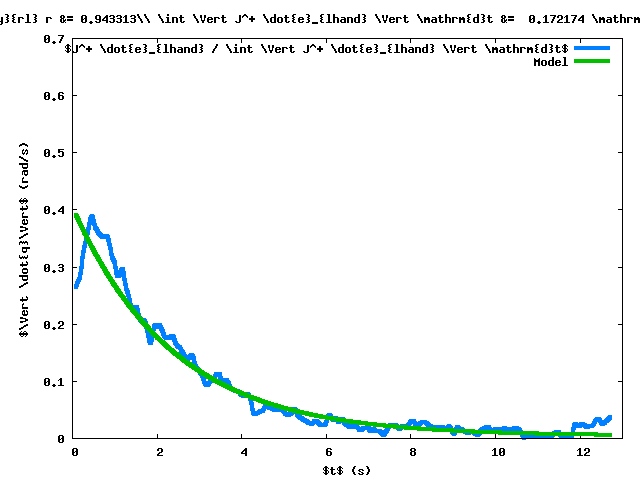
\includegraphics{img/exp1/RL/invJerror_taskLhand_0}}%
    \gplfronttext
  \end{picture}%
\endgroup

    }
  }\\
  \hline
  \subfigure{
    \resizebox{.43\textwidth}{!}{
      % GNUPLOT: LaTeX picture with Postscript
\begingroup
  \makeatletter
  \providecommand\color[2][]{%
    \GenericError{(gnuplot) \space\space\space\@spaces}{%
      Package color not loaded in conjunction with
      terminal option `colourtext'%
    }{See the gnuplot documentation for explanation.%
    }{Either use 'blacktext' in gnuplot or load the package
      color.sty in LaTeX.}%
    \renewcommand\color[2][]{}%
  }%
  \providecommand\includegraphics[2][]{%
    \GenericError{(gnuplot) \space\space\space\@spaces}{%
      Package graphicx or graphics not loaded%
    }{See the gnuplot documentation for explanation.%
    }{The gnuplot epslatex terminal needs graphicx.sty or graphics.sty.}%
    \renewcommand\includegraphics[2][]{}%
  }%
  \providecommand\rotatebox[2]{#2}%
  \@ifundefined{ifGPcolor}{%
    \newif\ifGPcolor
    \GPcolortrue
  }{}%
  \@ifundefined{ifGPblacktext}{%
    \newif\ifGPblacktext
    \GPblacktexttrue
  }{}%
  % define a \g@addto@macro without @ in the name:
  \let\gplgaddtomacro\g@addto@macro
  % define empty templates for all commands taking text:
  \gdef\gplbacktext{}%
  \gdef\gplfronttext{}%
  \makeatother
  \ifGPblacktext
    % no textcolor at all
    \def\colorrgb#1{}%
    \def\colorgray#1{}%
  \else
    % gray or color?
    \ifGPcolor
      \def\colorrgb#1{\color[rgb]{#1}}%
      \def\colorgray#1{\color[gray]{#1}}%
      \expandafter\def\csname LTw\endcsname{\color{white}}%
      \expandafter\def\csname LTb\endcsname{\color{black}}%
      \expandafter\def\csname LTa\endcsname{\color{black}}%
      \expandafter\def\csname LT0\endcsname{\color[rgb]{1,0,0}}%
      \expandafter\def\csname LT1\endcsname{\color[rgb]{0,1,0}}%
      \expandafter\def\csname LT2\endcsname{\color[rgb]{0,0,1}}%
      \expandafter\def\csname LT3\endcsname{\color[rgb]{1,0,1}}%
      \expandafter\def\csname LT4\endcsname{\color[rgb]{0,1,1}}%
      \expandafter\def\csname LT5\endcsname{\color[rgb]{1,1,0}}%
      \expandafter\def\csname LT6\endcsname{\color[rgb]{0,0,0}}%
      \expandafter\def\csname LT7\endcsname{\color[rgb]{1,0.3,0}}%
      \expandafter\def\csname LT8\endcsname{\color[rgb]{0.5,0.5,0.5}}%
    \else
      % gray
      \def\colorrgb#1{\color{black}}%
      \def\colorgray#1{\color[gray]{#1}}%
      \expandafter\def\csname LTw\endcsname{\color{white}}%
      \expandafter\def\csname LTb\endcsname{\color{black}}%
      \expandafter\def\csname LTa\endcsname{\color{black}}%
      \expandafter\def\csname LT0\endcsname{\color{black}}%
      \expandafter\def\csname LT1\endcsname{\color{black}}%
      \expandafter\def\csname LT2\endcsname{\color{black}}%
      \expandafter\def\csname LT3\endcsname{\color{black}}%
      \expandafter\def\csname LT4\endcsname{\color{black}}%
      \expandafter\def\csname LT5\endcsname{\color{black}}%
      \expandafter\def\csname LT6\endcsname{\color{black}}%
      \expandafter\def\csname LT7\endcsname{\color{black}}%
      \expandafter\def\csname LT8\endcsname{\color{black}}%
    \fi
  \fi
  \setlength{\unitlength}{0.0500bp}%
  \begin{picture}(7200.00,5040.00)%
    \gplgaddtomacro\gplbacktext{%
      \csname LTb\endcsname%
      \put(1210,704){\makebox(0,0)[r]{\strut{} 0}}%
      \put(1210,1229){\makebox(0,0)[r]{\strut{} 0.1}}%
      \put(1210,1754){\makebox(0,0)[r]{\strut{} 0.2}}%
      \put(1210,2279){\makebox(0,0)[r]{\strut{} 0.3}}%
      \put(1210,2805){\makebox(0,0)[r]{\strut{} 0.4}}%
      \put(1210,3330){\makebox(0,0)[r]{\strut{} 0.5}}%
      \put(1210,3855){\makebox(0,0)[r]{\strut{} 0.6}}%
      \put(1210,4380){\makebox(0,0)[r]{\strut{} 0.7}}%
      \put(1342,484){\makebox(0,0){\strut{} 0}}%
      \put(2192,484){\makebox(0,0){\strut{} 2}}%
      \put(3043,484){\makebox(0,0){\strut{} 4}}%
      \put(3893,484){\makebox(0,0){\strut{} 6}}%
      \put(4744,484){\makebox(0,0){\strut{} 8}}%
      \put(5594,484){\makebox(0,0){\strut{} 10}}%
      \put(6445,484){\makebox(0,0){\strut{} 12}}%
      \put(440,2542){\rotatebox{90}{\makebox(0,0){\strut{}$\Vert \dot{q}\Vert$ (rad/s)}}}%
      \put(4106,154){\makebox(0,0){\strut{}$t$ (s)}}%
      \put(4106,4710){\makebox(0,0){\strut{}$\begin{array}{rl} r &= 2.94667\\ \int \Vert J^+ \dot{e}_{lhand} \Vert \mathrm{d}t &=  0.167428 \mathrm{rad}\\ \end{array}$}}%
    }%
    \gplgaddtomacro\gplfronttext{%
      \csname LTb\endcsname%
      \put(5883,4207){\makebox(0,0)[r]{\strut{}$J^+ \dot{e}_{lhand} / \int \Vert J^+ \dot{e}_{lhand} \Vert \mathrm{d}t$}}%
      \csname LTb\endcsname%
      \put(5883,3987){\makebox(0,0)[r]{\strut{}Model}}%
    }%
    \gplbacktext
    \put(0,0){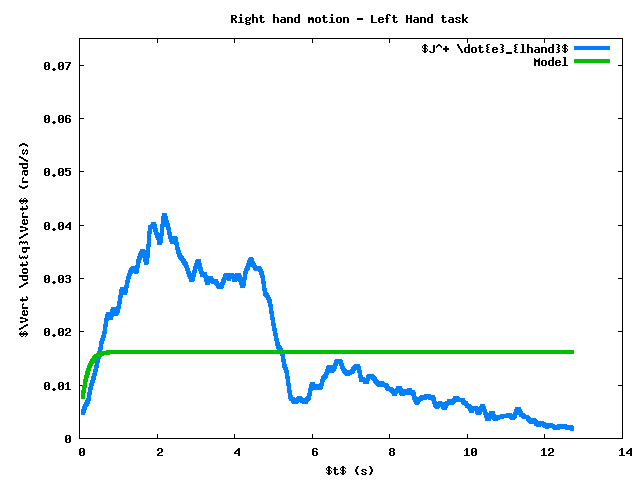
\includegraphics{img/exp1/R/invJerror_taskLhand_1}}%
    \gplfronttext
  \end{picture}%
\endgroup

    }
  }
  &
  \subfigure{
    \resizebox{.43\textwidth}{!}{
      % GNUPLOT: LaTeX picture with Postscript
\begingroup
  \makeatletter
  \providecommand\color[2][]{%
    \GenericError{(gnuplot) \space\space\space\@spaces}{%
      Package color not loaded in conjunction with
      terminal option `colourtext'%
    }{See the gnuplot documentation for explanation.%
    }{Either use 'blacktext' in gnuplot or load the package
      color.sty in LaTeX.}%
    \renewcommand\color[2][]{}%
  }%
  \providecommand\includegraphics[2][]{%
    \GenericError{(gnuplot) \space\space\space\@spaces}{%
      Package graphicx or graphics not loaded%
    }{See the gnuplot documentation for explanation.%
    }{The gnuplot epslatex terminal needs graphicx.sty or graphics.sty.}%
    \renewcommand\includegraphics[2][]{}%
  }%
  \providecommand\rotatebox[2]{#2}%
  \@ifundefined{ifGPcolor}{%
    \newif\ifGPcolor
    \GPcolortrue
  }{}%
  \@ifundefined{ifGPblacktext}{%
    \newif\ifGPblacktext
    \GPblacktexttrue
  }{}%
  % define a \g@addto@macro without @ in the name:
  \let\gplgaddtomacro\g@addto@macro
  % define empty templates for all commands taking text:
  \gdef\gplbacktext{}%
  \gdef\gplfronttext{}%
  \makeatother
  \ifGPblacktext
    % no textcolor at all
    \def\colorrgb#1{}%
    \def\colorgray#1{}%
  \else
    % gray or color?
    \ifGPcolor
      \def\colorrgb#1{\color[rgb]{#1}}%
      \def\colorgray#1{\color[gray]{#1}}%
      \expandafter\def\csname LTw\endcsname{\color{white}}%
      \expandafter\def\csname LTb\endcsname{\color{black}}%
      \expandafter\def\csname LTa\endcsname{\color{black}}%
      \expandafter\def\csname LT0\endcsname{\color[rgb]{1,0,0}}%
      \expandafter\def\csname LT1\endcsname{\color[rgb]{0,1,0}}%
      \expandafter\def\csname LT2\endcsname{\color[rgb]{0,0,1}}%
      \expandafter\def\csname LT3\endcsname{\color[rgb]{1,0,1}}%
      \expandafter\def\csname LT4\endcsname{\color[rgb]{0,1,1}}%
      \expandafter\def\csname LT5\endcsname{\color[rgb]{1,1,0}}%
      \expandafter\def\csname LT6\endcsname{\color[rgb]{0,0,0}}%
      \expandafter\def\csname LT7\endcsname{\color[rgb]{1,0.3,0}}%
      \expandafter\def\csname LT8\endcsname{\color[rgb]{0.5,0.5,0.5}}%
    \else
      % gray
      \def\colorrgb#1{\color{black}}%
      \def\colorgray#1{\color[gray]{#1}}%
      \expandafter\def\csname LTw\endcsname{\color{white}}%
      \expandafter\def\csname LTb\endcsname{\color{black}}%
      \expandafter\def\csname LTa\endcsname{\color{black}}%
      \expandafter\def\csname LT0\endcsname{\color{black}}%
      \expandafter\def\csname LT1\endcsname{\color{black}}%
      \expandafter\def\csname LT2\endcsname{\color{black}}%
      \expandafter\def\csname LT3\endcsname{\color{black}}%
      \expandafter\def\csname LT4\endcsname{\color{black}}%
      \expandafter\def\csname LT5\endcsname{\color{black}}%
      \expandafter\def\csname LT6\endcsname{\color{black}}%
      \expandafter\def\csname LT7\endcsname{\color{black}}%
      \expandafter\def\csname LT8\endcsname{\color{black}}%
    \fi
  \fi
  \setlength{\unitlength}{0.0500bp}%
  \begin{picture}(7200.00,5040.00)%
    \gplgaddtomacro\gplbacktext{%
      \csname LTb\endcsname%
      \put(1342,704){\makebox(0,0)[r]{\strut{} 0}}%
      \put(1342,1194){\makebox(0,0)[r]{\strut{} 0.01}}%
      \put(1342,1684){\makebox(0,0)[r]{\strut{} 0.02}}%
      \put(1342,2174){\makebox(0,0)[r]{\strut{} 0.03}}%
      \put(1342,2665){\makebox(0,0)[r]{\strut{} 0.04}}%
      \put(1342,3155){\makebox(0,0)[r]{\strut{} 0.05}}%
      \put(1342,3645){\makebox(0,0)[r]{\strut{} 0.06}}%
      \put(1342,4135){\makebox(0,0)[r]{\strut{} 0.07}}%
      \put(1474,484){\makebox(0,0){\strut{} 0}}%
      \put(2245,484){\makebox(0,0){\strut{} 2}}%
      \put(3016,484){\makebox(0,0){\strut{} 4}}%
      \put(3787,484){\makebox(0,0){\strut{} 6}}%
      \put(4557,484){\makebox(0,0){\strut{} 8}}%
      \put(5328,484){\makebox(0,0){\strut{} 10}}%
      \put(6099,484){\makebox(0,0){\strut{} 12}}%
      \put(6870,484){\makebox(0,0){\strut{} 14}}%
      \put(440,2542){\rotatebox{90}{\makebox(0,0){\strut{}$\Vert \dot{q}\Vert$ (rad/s)}}}%
      \put(4172,154){\makebox(0,0){\strut{}$t$ (s)}}%
      \put(4172,4710){\makebox(0,0){\strut{}Right and left hand motion - Left hand task}}%
    }%
    \gplgaddtomacro\gplfronttext{%
      \csname LTb\endcsname%
      \put(5883,4207){\makebox(0,0)[r]{\strut{}$J^+ \dot{e}_{lhand}$}}%
      \csname LTb\endcsname%
      \put(5883,3987){\makebox(0,0)[r]{\strut{}Model}}%
    }%
    \gplbacktext
    \put(0,0){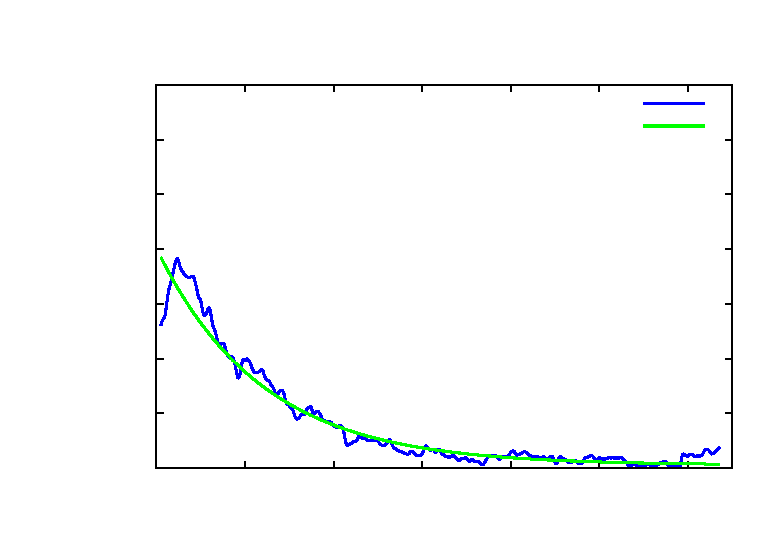
\includegraphics{img/exp1/RL/invJerror_taskLhand_1}}%
    \gplfronttext
  \end{picture}%
\endgroup

    }
  }\\
  \hline
  \subfigure{
    \resizebox{.43\textwidth}{!}{
      % GNUPLOT: LaTeX picture with Postscript
\begingroup
  \makeatletter
  \providecommand\color[2][]{%
    \GenericError{(gnuplot) \space\space\space\@spaces}{%
      Package color not loaded in conjunction with
      terminal option `colourtext'%
    }{See the gnuplot documentation for explanation.%
    }{Either use 'blacktext' in gnuplot or load the package
      color.sty in LaTeX.}%
    \renewcommand\color[2][]{}%
  }%
  \providecommand\includegraphics[2][]{%
    \GenericError{(gnuplot) \space\space\space\@spaces}{%
      Package graphicx or graphics not loaded%
    }{See the gnuplot documentation for explanation.%
    }{The gnuplot epslatex terminal needs graphicx.sty or graphics.sty.}%
    \renewcommand\includegraphics[2][]{}%
  }%
  \providecommand\rotatebox[2]{#2}%
  \@ifundefined{ifGPcolor}{%
    \newif\ifGPcolor
    \GPcolortrue
  }{}%
  \@ifundefined{ifGPblacktext}{%
    \newif\ifGPblacktext
    \GPblacktexttrue
  }{}%
  % define a \g@addto@macro without @ in the name:
  \let\gplgaddtomacro\g@addto@macro
  % define empty templates for all commands taking text:
  \gdef\gplbacktext{}%
  \gdef\gplfronttext{}%
  \makeatother
  \ifGPblacktext
    % no textcolor at all
    \def\colorrgb#1{}%
    \def\colorgray#1{}%
  \else
    % gray or color?
    \ifGPcolor
      \def\colorrgb#1{\color[rgb]{#1}}%
      \def\colorgray#1{\color[gray]{#1}}%
      \expandafter\def\csname LTw\endcsname{\color{white}}%
      \expandafter\def\csname LTb\endcsname{\color{black}}%
      \expandafter\def\csname LTa\endcsname{\color{black}}%
      \expandafter\def\csname LT0\endcsname{\color[rgb]{1,0,0}}%
      \expandafter\def\csname LT1\endcsname{\color[rgb]{0,1,0}}%
      \expandafter\def\csname LT2\endcsname{\color[rgb]{0,0,1}}%
      \expandafter\def\csname LT3\endcsname{\color[rgb]{1,0,1}}%
      \expandafter\def\csname LT4\endcsname{\color[rgb]{0,1,1}}%
      \expandafter\def\csname LT5\endcsname{\color[rgb]{1,1,0}}%
      \expandafter\def\csname LT6\endcsname{\color[rgb]{0,0,0}}%
      \expandafter\def\csname LT7\endcsname{\color[rgb]{1,0.3,0}}%
      \expandafter\def\csname LT8\endcsname{\color[rgb]{0.5,0.5,0.5}}%
    \else
      % gray
      \def\colorrgb#1{\color{black}}%
      \def\colorgray#1{\color[gray]{#1}}%
      \expandafter\def\csname LTw\endcsname{\color{white}}%
      \expandafter\def\csname LTb\endcsname{\color{black}}%
      \expandafter\def\csname LTa\endcsname{\color{black}}%
      \expandafter\def\csname LT0\endcsname{\color{black}}%
      \expandafter\def\csname LT1\endcsname{\color{black}}%
      \expandafter\def\csname LT2\endcsname{\color{black}}%
      \expandafter\def\csname LT3\endcsname{\color{black}}%
      \expandafter\def\csname LT4\endcsname{\color{black}}%
      \expandafter\def\csname LT5\endcsname{\color{black}}%
      \expandafter\def\csname LT6\endcsname{\color{black}}%
      \expandafter\def\csname LT7\endcsname{\color{black}}%
      \expandafter\def\csname LT8\endcsname{\color{black}}%
    \fi
  \fi
  \setlength{\unitlength}{0.0500bp}%
  \begin{picture}(7200.00,5040.00)%
    \gplgaddtomacro\gplbacktext{%
      \csname LTb\endcsname%
      \put(1210,704){\makebox(0,0)[r]{\strut{} 0}}%
      \put(1210,1229){\makebox(0,0)[r]{\strut{} 0.1}}%
      \put(1210,1754){\makebox(0,0)[r]{\strut{} 0.2}}%
      \put(1210,2279){\makebox(0,0)[r]{\strut{} 0.3}}%
      \put(1210,2805){\makebox(0,0)[r]{\strut{} 0.4}}%
      \put(1210,3330){\makebox(0,0)[r]{\strut{} 0.5}}%
      \put(1210,3855){\makebox(0,0)[r]{\strut{} 0.6}}%
      \put(1210,4380){\makebox(0,0)[r]{\strut{} 0.7}}%
      \put(1342,484){\makebox(0,0){\strut{} 0}}%
      \put(2192,484){\makebox(0,0){\strut{} 2}}%
      \put(3043,484){\makebox(0,0){\strut{} 4}}%
      \put(3893,484){\makebox(0,0){\strut{} 6}}%
      \put(4744,484){\makebox(0,0){\strut{} 8}}%
      \put(5594,484){\makebox(0,0){\strut{} 10}}%
      \put(6445,484){\makebox(0,0){\strut{} 12}}%
      \put(440,2542){\rotatebox{90}{\makebox(0,0){\strut{}$\Vert \dot{q}\Vert$ (rad/s)}}}%
      \put(4106,154){\makebox(0,0){\strut{}$t$ (s)}}%
      \put(4106,4710){\makebox(0,0){\strut{}$\begin{array}{rl} r &= 2.92974\\ \int \Vert J^+ \dot{e}_{lhand} \Vert \mathrm{d}t &=  0.159377 \mathrm{rad}\\ \end{array}$}}%
    }%
    \gplgaddtomacro\gplfronttext{%
      \csname LTb\endcsname%
      \put(5883,4207){\makebox(0,0)[r]{\strut{}$J^+ \dot{e}_{lhand} / \int \Vert J^+ \dot{e}_{lhand} \Vert \mathrm{d}t$}}%
      \csname LTb\endcsname%
      \put(5883,3987){\makebox(0,0)[r]{\strut{}Model}}%
    }%
    \gplbacktext
    \put(0,0){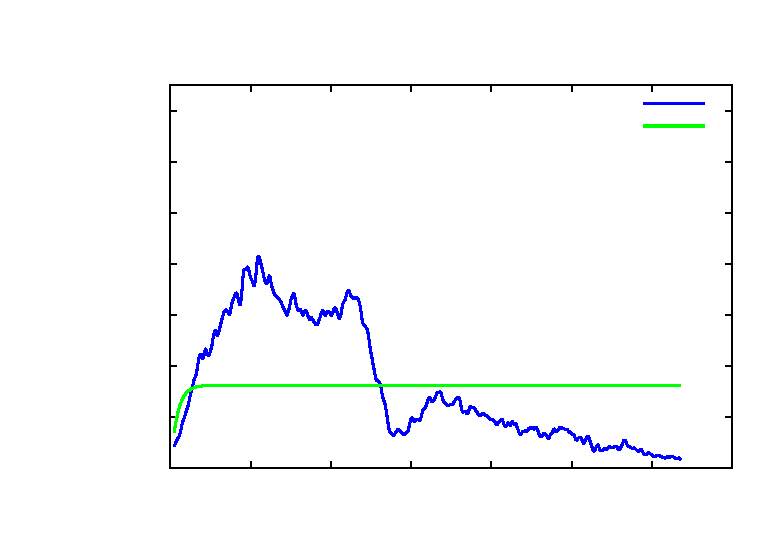
\includegraphics{img/exp1/R/invJerror_taskLhand_2}}%
    \gplfronttext
  \end{picture}%
\endgroup

    } 
  }
  &
  \subfigure{
    \resizebox{.43\textwidth}{!}{
      % GNUPLOT: LaTeX picture with Postscript
\begingroup
  \makeatletter
  \providecommand\color[2][]{%
    \GenericError{(gnuplot) \space\space\space\@spaces}{%
      Package color not loaded in conjunction with
      terminal option `colourtext'%
    }{See the gnuplot documentation for explanation.%
    }{Either use 'blacktext' in gnuplot or load the package
      color.sty in LaTeX.}%
    \renewcommand\color[2][]{}%
  }%
  \providecommand\includegraphics[2][]{%
    \GenericError{(gnuplot) \space\space\space\@spaces}{%
      Package graphicx or graphics not loaded%
    }{See the gnuplot documentation for explanation.%
    }{The gnuplot epslatex terminal needs graphicx.sty or graphics.sty.}%
    \renewcommand\includegraphics[2][]{}%
  }%
  \providecommand\rotatebox[2]{#2}%
  \@ifundefined{ifGPcolor}{%
    \newif\ifGPcolor
    \GPcolortrue
  }{}%
  \@ifundefined{ifGPblacktext}{%
    \newif\ifGPblacktext
    \GPblacktexttrue
  }{}%
  % define a \g@addto@macro without @ in the name:
  \let\gplgaddtomacro\g@addto@macro
  % define empty templates for all commands taking text:
  \gdef\gplbacktext{}%
  \gdef\gplfronttext{}%
  \makeatother
  \ifGPblacktext
    % no textcolor at all
    \def\colorrgb#1{}%
    \def\colorgray#1{}%
  \else
    % gray or color?
    \ifGPcolor
      \def\colorrgb#1{\color[rgb]{#1}}%
      \def\colorgray#1{\color[gray]{#1}}%
      \expandafter\def\csname LTw\endcsname{\color{white}}%
      \expandafter\def\csname LTb\endcsname{\color{black}}%
      \expandafter\def\csname LTa\endcsname{\color{black}}%
      \expandafter\def\csname LT0\endcsname{\color[rgb]{1,0,0}}%
      \expandafter\def\csname LT1\endcsname{\color[rgb]{0,1,0}}%
      \expandafter\def\csname LT2\endcsname{\color[rgb]{0,0,1}}%
      \expandafter\def\csname LT3\endcsname{\color[rgb]{1,0,1}}%
      \expandafter\def\csname LT4\endcsname{\color[rgb]{0,1,1}}%
      \expandafter\def\csname LT5\endcsname{\color[rgb]{1,1,0}}%
      \expandafter\def\csname LT6\endcsname{\color[rgb]{0,0,0}}%
      \expandafter\def\csname LT7\endcsname{\color[rgb]{1,0.3,0}}%
      \expandafter\def\csname LT8\endcsname{\color[rgb]{0.5,0.5,0.5}}%
    \else
      % gray
      \def\colorrgb#1{\color{black}}%
      \def\colorgray#1{\color[gray]{#1}}%
      \expandafter\def\csname LTw\endcsname{\color{white}}%
      \expandafter\def\csname LTb\endcsname{\color{black}}%
      \expandafter\def\csname LTa\endcsname{\color{black}}%
      \expandafter\def\csname LT0\endcsname{\color{black}}%
      \expandafter\def\csname LT1\endcsname{\color{black}}%
      \expandafter\def\csname LT2\endcsname{\color{black}}%
      \expandafter\def\csname LT3\endcsname{\color{black}}%
      \expandafter\def\csname LT4\endcsname{\color{black}}%
      \expandafter\def\csname LT5\endcsname{\color{black}}%
      \expandafter\def\csname LT6\endcsname{\color{black}}%
      \expandafter\def\csname LT7\endcsname{\color{black}}%
      \expandafter\def\csname LT8\endcsname{\color{black}}%
    \fi
  \fi
  \setlength{\unitlength}{0.0500bp}%
  \begin{picture}(7200.00,5040.00)%
    \gplgaddtomacro\gplbacktext{%
      \csname LTb\endcsname%
      \put(1342,704){\makebox(0,0)[r]{\strut{} 0}}%
      \put(1342,1194){\makebox(0,0)[r]{\strut{} 0.01}}%
      \put(1342,1684){\makebox(0,0)[r]{\strut{} 0.02}}%
      \put(1342,2174){\makebox(0,0)[r]{\strut{} 0.03}}%
      \put(1342,2665){\makebox(0,0)[r]{\strut{} 0.04}}%
      \put(1342,3155){\makebox(0,0)[r]{\strut{} 0.05}}%
      \put(1342,3645){\makebox(0,0)[r]{\strut{} 0.06}}%
      \put(1342,4135){\makebox(0,0)[r]{\strut{} 0.07}}%
      \put(1474,484){\makebox(0,0){\strut{} 0}}%
      \put(2245,484){\makebox(0,0){\strut{} 2}}%
      \put(3016,484){\makebox(0,0){\strut{} 4}}%
      \put(3787,484){\makebox(0,0){\strut{} 6}}%
      \put(4557,484){\makebox(0,0){\strut{} 8}}%
      \put(5328,484){\makebox(0,0){\strut{} 10}}%
      \put(6099,484){\makebox(0,0){\strut{} 12}}%
      \put(6870,484){\makebox(0,0){\strut{} 14}}%
      \put(440,2542){\rotatebox{90}{\makebox(0,0){\strut{}$\Vert \dot{q}\Vert$ (rad/s)}}}%
      \put(4172,154){\makebox(0,0){\strut{}$t$ (s)}}%
      \put(4172,4710){\makebox(0,0){\strut{}Right and left hand motion - Left hand task}}%
    }%
    \gplgaddtomacro\gplfronttext{%
      \csname LTb\endcsname%
      \put(5883,4207){\makebox(0,0)[r]{\strut{}$J^+ \dot{e}_{lhand}$}}%
      \csname LTb\endcsname%
      \put(5883,3987){\makebox(0,0)[r]{\strut{}Model}}%
    }%
    \gplbacktext
    \put(0,0){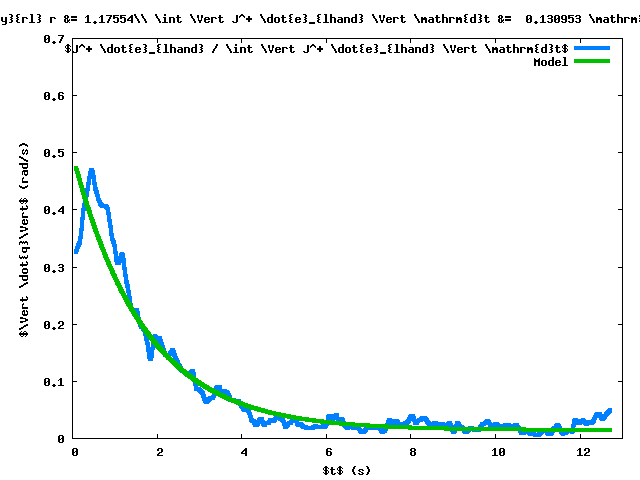
\includegraphics{img/exp1/RL/invJerror_taskLhand_2}}%
    \gplfronttext
  \end{picture}%
\endgroup

    }
  }\\ 
  \hline
  &
  \subfigure{
    \resizebox{.43\textwidth}{!}{
      % GNUPLOT: LaTeX picture with Postscript
\begingroup
  \makeatletter
  \providecommand\color[2][]{%
    \GenericError{(gnuplot) \space\space\space\@spaces}{%
      Package color not loaded in conjunction with
      terminal option `colourtext'%
    }{See the gnuplot documentation for explanation.%
    }{Either use 'blacktext' in gnuplot or load the package
      color.sty in LaTeX.}%
    \renewcommand\color[2][]{}%
  }%
  \providecommand\includegraphics[2][]{%
    \GenericError{(gnuplot) \space\space\space\@spaces}{%
      Package graphicx or graphics not loaded%
    }{See the gnuplot documentation for explanation.%
    }{The gnuplot epslatex terminal needs graphicx.sty or graphics.sty.}%
    \renewcommand\includegraphics[2][]{}%
  }%
  \providecommand\rotatebox[2]{#2}%
  \@ifundefined{ifGPcolor}{%
    \newif\ifGPcolor
    \GPcolortrue
  }{}%
  \@ifundefined{ifGPblacktext}{%
    \newif\ifGPblacktext
    \GPblacktexttrue
  }{}%
  % define a \g@addto@macro without @ in the name:
  \let\gplgaddtomacro\g@addto@macro
  % define empty templates for all commands taking text:
  \gdef\gplbacktext{}%
  \gdef\gplfronttext{}%
  \makeatother
  \ifGPblacktext
    % no textcolor at all
    \def\colorrgb#1{}%
    \def\colorgray#1{}%
  \else
    % gray or color?
    \ifGPcolor
      \def\colorrgb#1{\color[rgb]{#1}}%
      \def\colorgray#1{\color[gray]{#1}}%
      \expandafter\def\csname LTw\endcsname{\color{white}}%
      \expandafter\def\csname LTb\endcsname{\color{black}}%
      \expandafter\def\csname LTa\endcsname{\color{black}}%
      \expandafter\def\csname LT0\endcsname{\color[rgb]{1,0,0}}%
      \expandafter\def\csname LT1\endcsname{\color[rgb]{0,1,0}}%
      \expandafter\def\csname LT2\endcsname{\color[rgb]{0,0,1}}%
      \expandafter\def\csname LT3\endcsname{\color[rgb]{1,0,1}}%
      \expandafter\def\csname LT4\endcsname{\color[rgb]{0,1,1}}%
      \expandafter\def\csname LT5\endcsname{\color[rgb]{1,1,0}}%
      \expandafter\def\csname LT6\endcsname{\color[rgb]{0,0,0}}%
      \expandafter\def\csname LT7\endcsname{\color[rgb]{1,0.3,0}}%
      \expandafter\def\csname LT8\endcsname{\color[rgb]{0.5,0.5,0.5}}%
    \else
      % gray
      \def\colorrgb#1{\color{black}}%
      \def\colorgray#1{\color[gray]{#1}}%
      \expandafter\def\csname LTw\endcsname{\color{white}}%
      \expandafter\def\csname LTb\endcsname{\color{black}}%
      \expandafter\def\csname LTa\endcsname{\color{black}}%
      \expandafter\def\csname LT0\endcsname{\color{black}}%
      \expandafter\def\csname LT1\endcsname{\color{black}}%
      \expandafter\def\csname LT2\endcsname{\color{black}}%
      \expandafter\def\csname LT3\endcsname{\color{black}}%
      \expandafter\def\csname LT4\endcsname{\color{black}}%
      \expandafter\def\csname LT5\endcsname{\color{black}}%
      \expandafter\def\csname LT6\endcsname{\color{black}}%
      \expandafter\def\csname LT7\endcsname{\color{black}}%
      \expandafter\def\csname LT8\endcsname{\color{black}}%
    \fi
  \fi
  \setlength{\unitlength}{0.0500bp}%
  \begin{picture}(7200.00,5040.00)%
    \gplgaddtomacro\gplbacktext{%
      \csname LTb\endcsname%
      \put(1342,704){\makebox(0,0)[r]{\strut{} 0}}%
      \put(1342,1194){\makebox(0,0)[r]{\strut{} 0.01}}%
      \put(1342,1684){\makebox(0,0)[r]{\strut{} 0.02}}%
      \put(1342,2174){\makebox(0,0)[r]{\strut{} 0.03}}%
      \put(1342,2665){\makebox(0,0)[r]{\strut{} 0.04}}%
      \put(1342,3155){\makebox(0,0)[r]{\strut{} 0.05}}%
      \put(1342,3645){\makebox(0,0)[r]{\strut{} 0.06}}%
      \put(1342,4135){\makebox(0,0)[r]{\strut{} 0.07}}%
      \put(1474,484){\makebox(0,0){\strut{} 0}}%
      \put(2245,484){\makebox(0,0){\strut{} 2}}%
      \put(3016,484){\makebox(0,0){\strut{} 4}}%
      \put(3787,484){\makebox(0,0){\strut{} 6}}%
      \put(4557,484){\makebox(0,0){\strut{} 8}}%
      \put(5328,484){\makebox(0,0){\strut{} 10}}%
      \put(6099,484){\makebox(0,0){\strut{} 12}}%
      \put(6870,484){\makebox(0,0){\strut{} 14}}%
      \put(440,2542){\rotatebox{90}{\makebox(0,0){\strut{}$\Vert \dot{q}\Vert$ (rad/s)}}}%
      \put(4172,154){\makebox(0,0){\strut{}$t$ (s)}}%
      \put(4172,4710){\makebox(0,0){\strut{}Right and left hand motion - Left hand task}}%
    }%
    \gplgaddtomacro\gplfronttext{%
      \csname LTb\endcsname%
      \put(5883,4207){\makebox(0,0)[r]{\strut{}$J^+ \dot{e}_{lhand}$}}%
      \csname LTb\endcsname%
      \put(5883,3987){\makebox(0,0)[r]{\strut{}Model}}%
    }%
    \gplbacktext
    \put(0,0){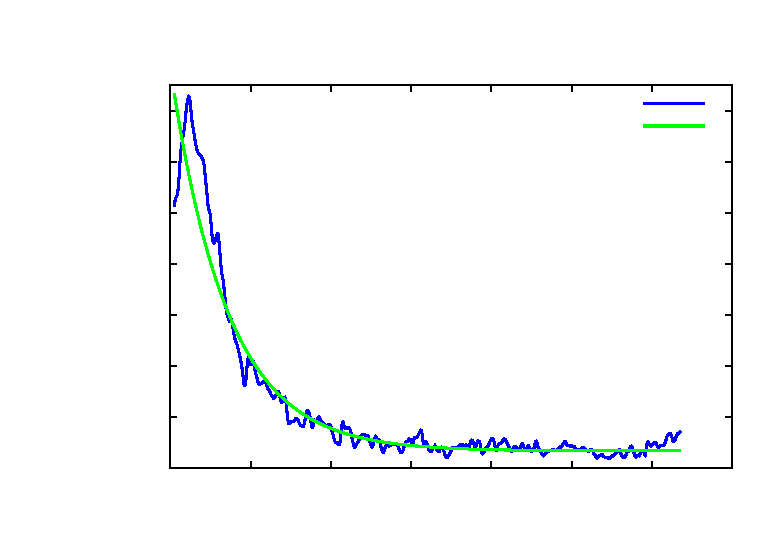
\includegraphics{img/exp1/RL/invJerror_taskLhand_3}}%
    \gplfronttext
  \end{picture}%
\endgroup

    }
  }\\
  \hline
\end{tabular}
\caption{Left hand task fiting.}
\end{figure*}

satan
satan satan satan satan satan satan satan satan satan satan satan
satan satan satan satan satan satan satan satan satan satan satan
satan satan satan satan satan satan satan satan satan satan satan
satan satan satan satan satan satan satan satan satan satan satan
satan satan satan satan satan satan satan satan satan satan satan
satan satan satan satan satan satan satan satan satan satan satan
satan satan satan satan satan satan satan satan satan satan satan
satan satan satan satan satan satan satan satan satan satan satan
satan satan satan satan satan satan satan satan satan satan satan
satan satan satan satan satan satan satan satan satan satan satan
satan satan satan satan satan satan satan satan satan satan satan
satan satan satan satan satan satan satan satan satan satan satan
satan satan satan satan satan satan satan satan satan satan satan

\begin{figure*}[t]
% GNUPLOT: LaTeX picture with Postscript
\begingroup
  \makeatletter
  \providecommand\color[2][]{%
    \GenericError{(gnuplot) \space\space\space\@spaces}{%
      Package color not loaded in conjunction with
      terminal option `colourtext'%
    }{See the gnuplot documentation for explanation.%
    }{Either use 'blacktext' in gnuplot or load the package
      color.sty in LaTeX.}%
    \renewcommand\color[2][]{}%
  }%
  \providecommand\includegraphics[2][]{%
    \GenericError{(gnuplot) \space\space\space\@spaces}{%
      Package graphicx or graphics not loaded%
    }{See the gnuplot documentation for explanation.%
    }{The gnuplot epslatex terminal needs graphicx.sty or graphics.sty.}%
    \renewcommand\includegraphics[2][]{}%
  }%
  \providecommand\rotatebox[2]{#2}%
  \@ifundefined{ifGPcolor}{%
    \newif\ifGPcolor
    \GPcolortrue
  }{}%
  \@ifundefined{ifGPblacktext}{%
    \newif\ifGPblacktext
    \GPblacktexttrue
  }{}%
  % define a \g@addto@macro without @ in the name:
  \let\gplgaddtomacro\g@addto@macro
  % define empty templates for all commands taking text:
  \gdef\gplbacktext{}%
  \gdef\gplfronttext{}%
  \makeatother
  \ifGPblacktext
    % no textcolor at all
    \def\colorrgb#1{}%
    \def\colorgray#1{}%
  \else
    % gray or color?
    \ifGPcolor
      \def\colorrgb#1{\color[rgb]{#1}}%
      \def\colorgray#1{\color[gray]{#1}}%
      \expandafter\def\csname LTw\endcsname{\color{white}}%
      \expandafter\def\csname LTb\endcsname{\color{black}}%
      \expandafter\def\csname LTa\endcsname{\color{black}}%
      \expandafter\def\csname LT0\endcsname{\color[rgb]{1,0,0}}%
      \expandafter\def\csname LT1\endcsname{\color[rgb]{0,1,0}}%
      \expandafter\def\csname LT2\endcsname{\color[rgb]{0,0,1}}%
      \expandafter\def\csname LT3\endcsname{\color[rgb]{1,0,1}}%
      \expandafter\def\csname LT4\endcsname{\color[rgb]{0,1,1}}%
      \expandafter\def\csname LT5\endcsname{\color[rgb]{1,1,0}}%
      \expandafter\def\csname LT6\endcsname{\color[rgb]{0,0,0}}%
      \expandafter\def\csname LT7\endcsname{\color[rgb]{1,0.3,0}}%
      \expandafter\def\csname LT8\endcsname{\color[rgb]{0.5,0.5,0.5}}%
    \else
      % gray
      \def\colorrgb#1{\color{black}}%
      \def\colorgray#1{\color[gray]{#1}}%
      \expandafter\def\csname LTw\endcsname{\color{white}}%
      \expandafter\def\csname LTb\endcsname{\color{black}}%
      \expandafter\def\csname LTa\endcsname{\color{black}}%
      \expandafter\def\csname LT0\endcsname{\color{black}}%
      \expandafter\def\csname LT1\endcsname{\color{black}}%
      \expandafter\def\csname LT2\endcsname{\color{black}}%
      \expandafter\def\csname LT3\endcsname{\color{black}}%
      \expandafter\def\csname LT4\endcsname{\color{black}}%
      \expandafter\def\csname LT5\endcsname{\color{black}}%
      \expandafter\def\csname LT6\endcsname{\color{black}}%
      \expandafter\def\csname LT7\endcsname{\color{black}}%
      \expandafter\def\csname LT8\endcsname{\color{black}}%
    \fi
  \fi
  \setlength{\unitlength}{0.0500bp}%
  \begin{picture}(7200.00,5040.00)%
    \gplgaddtomacro\gplbacktext{%
      \csname LTb\endcsname%
      \put(1606,704){\makebox(0,0)[r]{\strut{} 0}}%
      \put(1606,1372){\makebox(0,0)[r]{\strut{} 2e-05}}%
      \put(1606,2041){\makebox(0,0)[r]{\strut{} 4e-05}}%
      \put(1606,2709){\makebox(0,0)[r]{\strut{} 6e-05}}%
      \put(1606,3377){\makebox(0,0)[r]{\strut{} 8e-05}}%
      \put(1606,4046){\makebox(0,0)[r]{\strut{} 0.0001}}%
      \put(1738,484){\makebox(0,0){\strut{} 0}}%
      \put(2471,484){\makebox(0,0){\strut{} 2}}%
      \put(3204,484){\makebox(0,0){\strut{} 4}}%
      \put(3937,484){\makebox(0,0){\strut{} 6}}%
      \put(4671,484){\makebox(0,0){\strut{} 8}}%
      \put(5404,484){\makebox(0,0){\strut{} 10}}%
      \put(6137,484){\makebox(0,0){\strut{} 12}}%
      \put(6870,484){\makebox(0,0){\strut{} 14}}%
      \put(440,2542){\rotatebox{90}{\makebox(0,0){\strut{}$\Vert P\dot{q}\Vert$ (rad/s)}}}%
      \put(4304,154){\makebox(0,0){\strut{}$t$ (s)}}%
      \put(4304,4710){\makebox(0,0){\strut{}MOTION}}%
    }%
    \gplgaddtomacro\gplfronttext{%
      \csname LTb\endcsname%
      \put(5883,4207){\makebox(0,0)[r]{\strut{}$\Vert \dot{q} \Vert$}}%
      \csname LTb\endcsname%
      \put(5883,3987){\makebox(0,0)[r]{\strut{}$\Vert P_1\dot{q} \Vert$}}%
      \csname LTb\endcsname%
      \put(5883,3767){\makebox(0,0)[r]{\strut{}$\Vert P_2\dot{q} \Vert$}}%
      \csname LTb\endcsname%
      \put(5883,3547){\makebox(0,0)[r]{\strut{}$\Vert P_3\dot{q} \Vert$}}%
    }%
    \gplbacktext
    \put(0,0){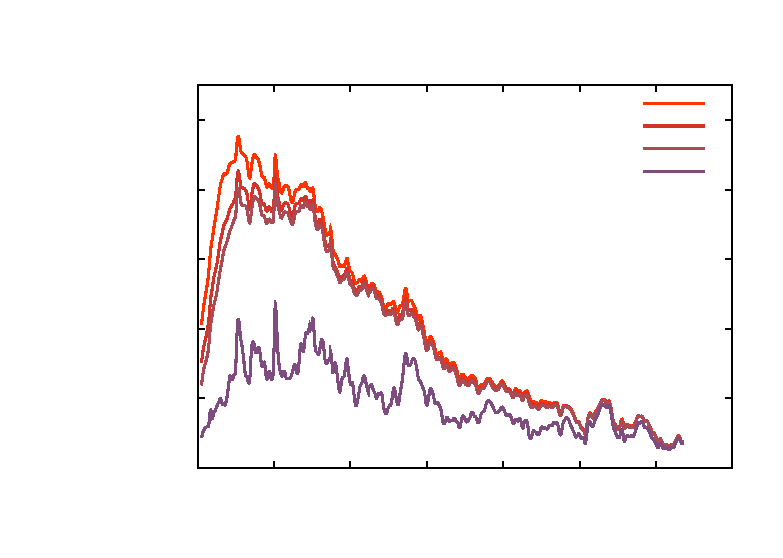
\includegraphics{img/exp1/R/PqdotNormsR}}%
    \gplfronttext
  \end{picture}%
\endgroup

\caption{Evolution of the norm of the motion after successively projecting the motion in the tasks null space for
the \emph{right hand} motion.}
\label{fig:exp1:PqdotNormsR}
\end{figure*}

satan
satan satan satan satan satan satan satan satan satan satan satan
satan satan satan satan satan satan satan satan satan satan satan
satan satan satan satan satan satan satan satan satan satan satan
satan satan satan satan satan satan satan satan satan satan satan
satan satan satan satan satan satan satan satan satan satan satan
satan satan satan satan satan satan satan satan satan satan satan
satan satan satan satan satan satan satan satan satan satan satan
satan satan satan satan satan satan satan satan satan satan satan
satan satan satan satan satan satan satan satan satan satan satan
satan satan satan satan satan satan satan satan satan satan satan
satan satan satan satan satan satan satan satan satan satan satan
satan

\begin{figure*}[t]
% GNUPLOT: LaTeX picture with Postscript
\begingroup
  \makeatletter
  \providecommand\color[2][]{%
    \GenericError{(gnuplot) \space\space\space\@spaces}{%
      Package color not loaded in conjunction with
      terminal option `colourtext'%
    }{See the gnuplot documentation for explanation.%
    }{Either use 'blacktext' in gnuplot or load the package
      color.sty in LaTeX.}%
    \renewcommand\color[2][]{}%
  }%
  \providecommand\includegraphics[2][]{%
    \GenericError{(gnuplot) \space\space\space\@spaces}{%
      Package graphicx or graphics not loaded%
    }{See the gnuplot documentation for explanation.%
    }{The gnuplot epslatex terminal needs graphicx.sty or graphics.sty.}%
    \renewcommand\includegraphics[2][]{}%
  }%
  \providecommand\rotatebox[2]{#2}%
  \@ifundefined{ifGPcolor}{%
    \newif\ifGPcolor
    \GPcolortrue
  }{}%
  \@ifundefined{ifGPblacktext}{%
    \newif\ifGPblacktext
    \GPblacktexttrue
  }{}%
  % define a \g@addto@macro without @ in the name:
  \let\gplgaddtomacro\g@addto@macro
  % define empty templates for all commands taking text:
  \gdef\gplbacktext{}%
  \gdef\gplfronttext{}%
  \makeatother
  \ifGPblacktext
    % no textcolor at all
    \def\colorrgb#1{}%
    \def\colorgray#1{}%
  \else
    % gray or color?
    \ifGPcolor
      \def\colorrgb#1{\color[rgb]{#1}}%
      \def\colorgray#1{\color[gray]{#1}}%
      \expandafter\def\csname LTw\endcsname{\color{white}}%
      \expandafter\def\csname LTb\endcsname{\color{black}}%
      \expandafter\def\csname LTa\endcsname{\color{black}}%
      \expandafter\def\csname LT0\endcsname{\color[rgb]{1,0,0}}%
      \expandafter\def\csname LT1\endcsname{\color[rgb]{0,1,0}}%
      \expandafter\def\csname LT2\endcsname{\color[rgb]{0,0,1}}%
      \expandafter\def\csname LT3\endcsname{\color[rgb]{1,0,1}}%
      \expandafter\def\csname LT4\endcsname{\color[rgb]{0,1,1}}%
      \expandafter\def\csname LT5\endcsname{\color[rgb]{1,1,0}}%
      \expandafter\def\csname LT6\endcsname{\color[rgb]{0,0,0}}%
      \expandafter\def\csname LT7\endcsname{\color[rgb]{1,0.3,0}}%
      \expandafter\def\csname LT8\endcsname{\color[rgb]{0.5,0.5,0.5}}%
    \else
      % gray
      \def\colorrgb#1{\color{black}}%
      \def\colorgray#1{\color[gray]{#1}}%
      \expandafter\def\csname LTw\endcsname{\color{white}}%
      \expandafter\def\csname LTb\endcsname{\color{black}}%
      \expandafter\def\csname LTa\endcsname{\color{black}}%
      \expandafter\def\csname LT0\endcsname{\color{black}}%
      \expandafter\def\csname LT1\endcsname{\color{black}}%
      \expandafter\def\csname LT2\endcsname{\color{black}}%
      \expandafter\def\csname LT3\endcsname{\color{black}}%
      \expandafter\def\csname LT4\endcsname{\color{black}}%
      \expandafter\def\csname LT5\endcsname{\color{black}}%
      \expandafter\def\csname LT6\endcsname{\color{black}}%
      \expandafter\def\csname LT7\endcsname{\color{black}}%
      \expandafter\def\csname LT8\endcsname{\color{black}}%
    \fi
  \fi
  \setlength{\unitlength}{0.0500bp}%
  \begin{picture}(7200.00,5040.00)%
    \gplgaddtomacro\gplbacktext{%
      \csname LTb\endcsname%
      \put(1606,704){\makebox(0,0)[r]{\strut{} 0}}%
      \put(1606,1372){\makebox(0,0)[r]{\strut{} 2e-05}}%
      \put(1606,2041){\makebox(0,0)[r]{\strut{} 4e-05}}%
      \put(1606,2709){\makebox(0,0)[r]{\strut{} 6e-05}}%
      \put(1606,3377){\makebox(0,0)[r]{\strut{} 8e-05}}%
      \put(1606,4046){\makebox(0,0)[r]{\strut{} 0.0001}}%
      \put(1738,484){\makebox(0,0){\strut{} 0}}%
      \put(2471,484){\makebox(0,0){\strut{} 2}}%
      \put(3204,484){\makebox(0,0){\strut{} 4}}%
      \put(3937,484){\makebox(0,0){\strut{} 6}}%
      \put(4671,484){\makebox(0,0){\strut{} 8}}%
      \put(5404,484){\makebox(0,0){\strut{} 10}}%
      \put(6137,484){\makebox(0,0){\strut{} 12}}%
      \put(6870,484){\makebox(0,0){\strut{} 14}}%
      \put(440,2542){\rotatebox{90}{\makebox(0,0){\strut{}$\Vert P\dot{q}\Vert$ (rad/s)}}}%
      \put(4304,154){\makebox(0,0){\strut{}$t$ (s)}}%
      \put(4304,4710){\makebox(0,0){\strut{}$\Vert P_i \dot{q} \Vert$ for \emph{both hands} motion.}}%
    }%
    \gplgaddtomacro\gplfronttext{%
      \csname LTb\endcsname%
      \put(5883,4207){\makebox(0,0)[r]{\strut{}$\Vert \dot{q} \Vert$}}%
      \csname LTb\endcsname%
      \put(5883,3987){\makebox(0,0)[r]{\strut{}$\Vert P_1\dot{q} \Vert$}}%
      \csname LTb\endcsname%
      \put(5883,3767){\makebox(0,0)[r]{\strut{}$\Vert P_2\dot{q} \Vert$}}%
      \csname LTb\endcsname%
      \put(5883,3547){\makebox(0,0)[r]{\strut{}$\Vert P_3\dot{q} \Vert$}}%
      \csname LTb\endcsname%
      \put(5883,3327){\makebox(0,0)[r]{\strut{}$\Vert P_4\dot{q} \Vert$}}%
    }%
    \gplbacktext
    \put(0,0){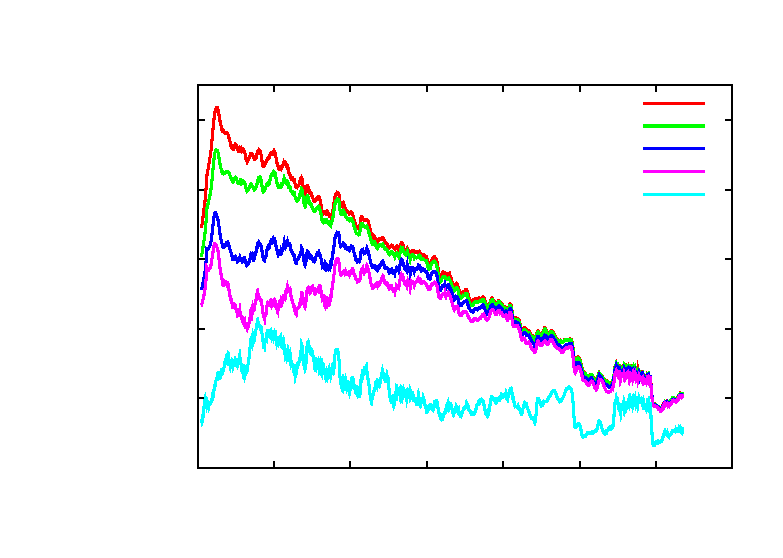
\includegraphics{img/exp1/RL/PqdotNormsRL}}%
    \gplfronttext
  \end{picture}%
\endgroup

\caption{Evolution of the norm of the motion after successively projecting the motion in the tasks null space for
the \emph{both hands} motion.}
\label{fig:exp1:PqdotNormsRL}
\end{figure*}

satan satan satan satan satan satan satan satan satan satan satan
satan satan satan satan satan satan satan satan satan satan satan
satan satan satan satan satan satan satan satan satan satan satan
satan satan satan satan satan satan satan satan satan satan satan
satan satan satan satan satan satan satan satan satan satan satan
satan satan satan satan satan satan satan satan satan satan satan
satan satan satan satan satan satan satan satan satan satan satan
satan satan satan satan satan satan satan satan satan satan satan
satan satan satan satan satan satan satan satan satan satan satan
satan satan satan satan satan satan satan satan satan satan satan
satan satan satan satan satan satan satan satan satan satan satan
satan

\bibliographystyle{unsrt}
\bibliography{biblio}

\end{document}
